\documentclass[utf8]{gradu3}

\usepackage[utf8]{inputenc}
\usepackage{graphicx} % kuvien mukaan ottamista varten
\usepackage{amsmath} % hyödyllinen jos tekstisi sisältää matikkaa,
                     % ei pakollinen
\usepackage{booktabs} % hyvä kauniiden taulukoiden tekemiseen
\usepackage{comment}
\usepackage{tikz}
\usepackage{tabularray}
\usepackage{xcolor}

\usepackage{tabularx}
\usepackage{ragged2e}
\usepackage{adjustbox}
\usepackage{lipsum}
\usepackage{longtable}
\usepackage{array}

% HUOM! Tämän tulee olla viimeinen \usepackage koko dokumentissa!
\usepackage[bookmarksopen,bookmarksnumbered,linktocpage]{hyperref}

\addbibresource{gradulahteet.bib} % Lähdetietokannan tiedostonimi


\begin{document}

\title{Systemaattinen kirjallisuuskatsaus ohjelmistokehitysalan perehdytyskäytännöistä (v. 0.6.2)}

\translatedtitle{Systematic Literature Review of Onboarding Practices in Software Engineering}
\studyline{Ohjelmisto- ja tietoliikennetekniikan opintosuunta}
\avainsanat{perehdyttäminen, uudet työntekijät, ohjelmistokehitys, Pro gradu -tutkielmat, systemaattiset kirjallisuuskatsaukset}
\keywords{onboarding, newcomers, software development, Master’s Theses, systematic literature reviews}

\tiivistelma{Tutkielmassa toteutettiin systemaattinen kirjallisuuskatsaus, jossa tutkittiin ohjelmistokehitysalan perehdytyskäytäntöjä. Katsauksessa tunnistettiin 45 perehdytyskäytäntöä, jotka luokiteltiin sosialisaatioresurssiteorian eri ulottuvuuksiin. Eniten tunnistettiin käytäntöjä, jotka liittyvät mentorointiin, uusille tulokkaille annettaviin tehtäviin ja palautteen antamiseen. Lisäksi tulokset toivat esiin myös tulokkaiden keskinäisen oppimisen, joka tutkielmassa määriteltiin sosialisaatioresurssien teoriaa täydentäväksi ulottuvuudeksi.}
\abstract{In this thesis a systematic literature review was conducted to investigate the practices of newcomer onboarding in software engineering. The review identified 45 onboarding practices, categorized along the different dimensions of the Socialization Resource Theory. Practices related to mentoring, the characteristics of tasks assigned to newcomers and providing them with feedback were the most frequently identified. In addition, the results also highlighted shared learning among newcomers, which was defined in the thesis as a complementary dimension to the previous theory.}

\author{Jessica Sarlin}
\contactinformation{\texttt{jessica.sarlin@gmail.com}}

\supervisor{Antti-Jussi Lakanen}

\maketitle

\mainmatter

\chapter{Johdanto}

Hyvä perehdytys työsuhteen alkaessa on tärkeää niin työntekijälle kuin työnantajallekin, jotta uusi tulokas saavuttaa tarvitsemansa edellytykset menestyäkseen työtehtävissään. Työyhteisöissä on erilaisia käytäntöjä perehdytyksen järjestämiseen. Tulokkaille voidaan järjestää esimerkiksi perehdytyssessioita tai nimetty mentori. Tulokas omaksuu vähitellen työssä tarvittavat tiedot, taidot, asenteet ja toimintatavat. Tätä oppimis- ja sopeutumisprosessia kutsutaan \textit{organisatoriseksi sosialisaatioksi} %
\parencites%
    {wanberg-2012}%
    {chao-2012}%
\relax.
%
Sen onnistumista voidaan edistää panostamalla hyvään perehdytykseen %
\parencites%
    {saks-gruman-2012}%
    {bauer-ym-2007}%
    {wanberg-2012}%
\relax.
%

Ohjelmistokehitysalalla tulokkailla on edessään haastava sosialisaatioprosessi, sillä työskentely vaatii monia vaikeita taitoja
%
\parencites%
    [][]{swebok}%
    {gregory-ym-2020}%
    {begel-simon-2008-all-over-again}%
\relax.
%
Perehdyttäminen jää kuitenkin usein vähäiseksi ja tulokkaat jäävät ponnistelemaan haastavassa toimintaympäristössä yksin %
\parencites%
    {buchan-ym-2019}%
    {dagenais-ym-2010}%
    {begel-simon-2008}%
\relax.
%
Tulokkaita turhauttaa myös riittämätön tekninen dokumentaatio \parencite{ju-ym-2021} sekä tiedon paljous ja vaikeudet ymmärtää oppimansa merkitystä oman työnsä kannalta \parencite{viviani-murphy-2019}. Usein tulokkaalle nimetään mentoriksi kokenut ohjelmistokehittäjä, mutta arvokkaan työajan käyttäminen tulokkaiden perehdyttämiseen heikentää mentorin tuottavuutta huomattavasti \parencite{medeiros-2021}. Vahvasti mentorointiin perustuva perehdytys saattaa muodostua mentorille itselleen taakaksi \parencite{viviani-murphy-2019}. Lisäksi monet tulokkaat kokevat opiskeluidensa annin riittämättömäksi työelämän haasteisiin nähden \parencite{craig-ym-2018}. Hyvä perehdytys on siis ensiarvoisen tärkeää.

Tässä tutkielmassa toteutettiin systemaattinen kirjallisuuskatsaus, jonka tuloksena havaittiin 45 alan yrityksissä käytettyä perehdytyskäytäntöä. Ne jaoteltiin sosialisaatioresurssien teorian \textcite{saks-gruman-2012} seitsemääntoista ulottuvuuteen pohjautuen. Useimmat käytännöt liittyivät mentorointiin, tulokkaille annettaviin työtehtäviin ja niiden luonteeseen sekä tulokkaalle annettavaan palautteeseen. Lisäksi tuloksissa korostui tulokkaiden keskinäinen oppiminen, joka tässä katsauksessa määriteltiin sosialisaatioresurssien teoriaa täydentäväksi ulottuvuudeksi.

Katsauksen tulokset antavat tietoa yritysten perehdytyskäytännöistä ja täydentävät aiempaa tutkimusta, joka on keskittynyt avoimen lähdekoodin yhteisöjen perehdyttämiskäytäntöihin. Tulosten perusteella organisaatioissa voidaan vahvistaa tulokkaiden perehdytyskäytäntöjä.

Tutkielman luvussa \ref{paaluku-teoria} rakennetaan tutkielman teoreettista viitekehystä käsittelemällä perehdyttämistä, organisatorista sosialisaatiota ja näiden välistä yhteyttä sekä perehdytyksen erityisyyttä ohjelmistokehityksen alalla. Lisäksi esitellään sosialisaatioresurssien teoria \parencite{saks-gruman-2012}. Luvussa \ref{paaluku-protokolla} esitellään systemaattisen kirjallisuuskatsauksen tutkimusprotokolla ja kuvaillaan tutkimuksen tiedonkeruuta. Luku \ref{paaluku-tulokset} esittelee katsauksen tulokset. Luvussa \ref{paaluku-pohdinta} luodaan synteesiä tuloksista ja pohditaan niiden käytännöllisiä merkityksiä. Tutkielman päättää luku \ref{paaluku-paatanta}, jossa tehdään yhteenvetoa tuloksista ja niihin liittyvistä rajoitteista sekä arvioidaan katsauksessa käytettyä tutkimusprotokollaa ja tutkimuksen eettisiä ulottuvuuksia.

\chapter{Teoriaosa}
\label{paaluku-teoria}

Tässä luvussa käsitellään perehdyttämisen haasteita ohjelmistoalalla sekä perehdyttämisen käsitettä, tärkeyttä ja hyötyjä. Tulokkaiden perehdytyskäytäntöjä jäsennetään sosialisaatioresurssien teorian \parencite{saks-gruman-2012} mukaisesti. Tulokas (engl. \textit{newcomer}) on kirjallisuudessa usein käytetty termi %
\parencites%
    [mm.][]{matturro-ym-2017}%
    {bauer-erdogan-2012}%
    {begel-simon-2008-all-over-again}%
    {steinmacher-ym-2015}%
    {britto-ym-2019}%
\relax.
%
Tässä katsauksessa sillä tarkoitetaan uutta työntekijää. Termi ei erottele sitä, onko työntekijä vastavalmistunut, juniori, kokenut vai kenties siirtynyt organisaation sisällä tehtävästä toiseen.

\section{Perehdyttämisen erityisyys ohjelmistokehityksessä}
\label{luku-perehdyttämisen-erityisyys-ohjelmistoalalla}

Miksi tulokkaiden perehdyttäminen on ohjelmistokehitysalalla erityisen haastavaa? Ohjelmistokehitys on luonteeltaan haastavaa ja tietointensiivistä asiantuntijatyötä \parencite{viana-ym-2014}, jonka perustaitojen kuten ohjelmoinnin, testaamisen ja virheenkorjauksen sekä näihin liittyvien työkalujen ja käytäntöjen lisäksi kehittäjien on osattava laaja joukko muitakin taitoja kuten kyky laatia kattavia vaatimusmäärittelyjä, omaksua nopeasti asioita ja kommunikoida tästä kaikesta eri tahoille %
\parencites%
    {tejera-hernández-ym-2018}%
    {begel-simon-2008-all-over-again}%
\relax.
%
Myös työssä käytettävien teknologioiden nopea kehitys asettaa vaatimuksia työntekijöiden ja organisaatioiden oppimiselle ja kehittymiselle \parencite{tejera-hernández-ym-2018}. \textcite{swebok} ovat toimittaneet IEEE-järjestön julkaiseman SWEBOK (Software Engineering Body of Knowledge) -julkaisun, joka kuvaa ohjelmistokehityksen yleiset osaamisvaatimukset. Ne on jaettu 15 osa-alueeseen kuten ohjelmistokehityksen prosessit, vaatimusmäärittely, suunnittelu, testaus, ylläpito, konfiguraatioidenhallinta, ammattikäytännöt ja laadunvarmistus \parencite{swebok}. Myös \textcite{gregory-ym-2020} toteavat, että ohjelmistokehittäjältä vaaditaan korkeatasoista teknistä taitoa, laajaa tietämystä, vahvaa kokemusta ja kohdealuetuntemusta. 

Ohjelmistokehittäjän työ tosiaan vaatii monia taitoja. Alan opinnot antavat vain perustaidot alalla työskentelyyn \parencite{begel-simon-2008-all-over-again}. Ammattiosaamisen saavuttaminen vaatii aikaa ja harjoitusta. Esimerkiksi \textcite{bologa-lupu-2014} toteavat, että kehittyminen juniorista osaajaksi kestää tyypillisesti noin kaksi vuotta. \textcite{britto-ym-2020} taas mainitsevat sen voivan kestää 3--5 vuotta. Lisäksi voidaan todeta, että ohjelmistokehittäjillä on moninaisia koulutustaustoja \parencite{barnes-ym-2022}, mikä myös asettaa vaatimuksia perehdytykselle. Osa kehittäjistä itseoppineita ja osa valmistunut erilaisista oppilaitoksista kuten ammattikouluista, ammattikorkeakouluista tai yliopistoista. Myös nk. bootcamp-tyyppinen intensiivikurssitus tuottaa ohjelmistoalan osaamista \parencite{lyon-green-2021}.

Nykyisin ohjelmistotekniikkaa käytetään mitä erilaisimmissa yhteyksissä. Esimerkiksi yrityksen toiminnanohjausjärjestelmän, mobiilipelin ja auton ajotietokoneen ohjelmistot poikkeavat toisistaan paljon. Näin erilaisten ohjelmistojen kehittämiseenkin toki pätevät erilaiset lainalaisuudet. Tämän vuoksi ohjelmistokehitystä tehdään eri organisaatioissa eri painotuksin, mikä asettaa vaatimuksia organisaatioiden perehdytyskäytännöille. Mikään oppilaitos ei voi tuottaa täysin valmiita osaajia, vaan organisaatioiden perehdytyskäytännöillä on tässä tärkeä rooli.

\section{Tulokkaiden haasteet ohjelmistoalalla}
\label{luku-tulokkaiden-haasteet}

Ohjelmistokehittäjät kohtaavat ensimmäisissä työpaikoissaan monenlaisia haasteita eri osa-alueilla, joita ovat muun muassa tiedonhankinta, dokumentaatio, kohdealueen tuntemus, kognitiivinen kuormitus, ammattiosaaminen sekä kommunikointi. 

\textbf{Tiedonhankinta} on tulokkaille haastavaa, sillä heidän on vaikea kysyä oikeita kysymyksiä oikea-aikaisesti, kysyä riittävä määrä tarkentavia kysymyksiä ja ymmärtää, keneltä eri asioista ylipäätään kannattaa kysyä %
\parencites%
    {ju-ym-2021}%
    {britto-ym-2019}%
    {craig-ym-2018}%
    {matturro-ym-2017}%
    {dagenais-ym-2010}%
    {begel-simon-2008}%
\relax
%
. Tulokkaan voi olla myös vaikea huomata jääneensä jumiin ja tarvitsevansa apua \parencite{begel-simon-2008}. Osa tulokkaista myös jättää  kysymyksiä esittämättä välttääkseen näyttämästä osaamattomuuttaan 
\parencites%
    {radermacher-ym-2015}%
    {begel-simon-2008}%
\relax.
%
\textcite{dagenais-ym-2010} toteavat, että usein käy myös niin, että henkilö joka olisi paras vastaamaan kysymykseen, ei enää työskentele organisaatiossa. Tässä tilanteessa kattava tekninen dokumentaatio voisi olla avuksi, mutta sitä ei välttämättä ole saatavilla. Haasteita voi aiheuttaa niukka, kokonaan puuttuva, vaikeaselkoisesti jäsennetty, vanhentunut tai ylimalkainen dokumentaatio %
\parencites%
    {matturro-ym-2017}%
    {dagenais-ym-2010}%
    {begel-simon-2008}%
\relax
%.
. Ohjelmiston vaatimusmäärittely on jopa voitu jättää kokonaan dokumentoimatta \parencite{matturro-ym-2017}.

\textcite{matturro-ym-2017} sekä \textcite{dagenais-ym-2010} toteavat, että puutteet kehitettävän ohjelmiston \textbf{kohdealueen tuntemuksessa} aiheuttavat tulokkaille pulmia. Heidän voi olla vaikea hahmottaa ohjelmiston käyttötarkoitusta, sen kokonaiskuvaa tai ongelmia, joita ohjelmiston käyttämisellä pyritään ratkaisemaan \parencite{matturro-ym-2017}.

\textbf{Ammattiosaamisen puutteet} vaikeuttavat myös tulokkaiden työskentelyä. Kirjallisuudessa
on mainittu erityisesti versionhallintaan, ohjelmistotestaukseen, lähdekoodissa navigoimiseen, paikallisen kehitysympäristön konfigurointiin, ohjelmistokehityksen hallintatyökalujen käyttöön ja ohjelmistokehitysprosesseissa toimimiseen liittyvien osaamisen puutteita  %
\parencites%
    {craig-ym-2018}%
    {matturro-ym-2017}%
    {dagenais-ym-2010}%
    {begel-simon-2008}%
\relax
% 
. Myös olemassaolevan lähdekoodin suuri määrä, sen kompleksisuus ja sen nk. legacy-piirteisyys aiheuttavat pulmia tulokkaille %
\parencites%
    {britto-ym-2019}%
    {viviani-murphy-2019}%
    {craig-ym-2018}
    {begel-simon-2008}%
\relax.
%.
\textcite{craig-ym-2018} kertovat, että tulokkaat ovat opiskeluaikanaan voineet saada vain niukalti kokemusta ryhmätyöskentelystä, jonka vuoksi myös työelämässä heidän on vaikeaa toimia osana ryhmää.

Perehtyminen aiheuttaa tulokkaille \textbf{kognitiivista kuormitusta} eri tavoin. \textcite{dagenais-ym-2010} sekä \textcite{begel-simon-2008} korostavat, että tulokkaan on omaksuttava suuria määriä tietoja kerralla. Muistiinpanojen ja muiden dokumenttien laatiminen ja organisointi on myös haastavaa \parencite{radermacher-ym-2015}. Jos perehdytys tapahtuu pienissä, strukturoimattomissa hetkissä muun työn ohella, oppiminen tapahtuu sattumanvaraisesti ja vailla jäsennystä \parencite{begel-simon-2008}. \textcite{craig-ym-2018} ja \textcite{britto-ym-2019} huomauttavat, että kehitettävien tietojärjestelmien suuri koko ja monimutkaisuus aiheuttavat haasteita tulokkaiden työskentelylle. Ohjelmistokehitystiimit saattavat myös muuttua jatkuvasti, mikä vaikeuttaa tulokkaiden oppimista \parencite{britto-ym-2019}.

\textcite{radermacher-ym-2015} toteavat tulokkaiden kokevan haasteita niin kirjallisessa, suullisessa kuin asiakkaidenkin kanssa tapahtuvassa \textbf{kommunikoinnissa}. \textcite{begel-simon-2008} mainitsevat, että vasta-alkajilla on vaikeuksia hahmottaa kuhunkin tilanteeseen sopivaa detaljien tasoa: toisinaan yksityiskohtaisen tiedon puute aiheuttaa väärinkäsityksiä ja toisinaan taas yksityiskohtiin takertuminen estää aiheen laajempaa käsittelyä. \textcite{begel-simon-2008} myös kertovat, että tulokkaiden tulee oppia tiettyä assertiivisuutta eli jämäkkyyttä, jotta he pystyvät sekä rajaamaan omaa työtään (sen sijaan että ottaisivat kollegoidensa pyynnöstä uusia työtehtäviä välittömästi työn alle) että toimimaan aktiivisesti saadakseen tuottamansa ohjelmistokoodin katselmoiduksi (sen sijaan että katselmointi jäisi tekemättä kollegoiden muiden kiireiden vuoksi). \textcite{moe-ym-2020} taas mainitsevat globaalisti hajautetun ohjelmistokehityksen osalta myös haasteet viestintätyökalujen toimivuudessa. \textcite{matturro-ym-2017} toteavat ohjelmistokehitystiimin kokeneiden jäsenten viestivän tulokkaalle vain niukalti tietoa kehitettävään ohjelmistoon liittyvistä muutoksista, ongelmista ja aiemmin tehdyistä päätöksistä.



\section{Organisatorisen sosialisaation ja perehdyttämisen käsitteet}
\label{luku-organisatorinen-sosialisaatio-ja-perehdyttäminen}

Tulokkaita koskevassa kirjallisuudessa nousevat usein esiin organisatorisen sosialialisaation (engl. \textit{organizational socialization}) ja perehdyttämisen (engl. \textit{onboarding}) käsitteet. Tässä luvussa käsitellään sitä, miten niitä ja niihin liittyviä ilmiöitä on pyritty käsitteellistämään ja määrittelemään.

\textbf{Sosialisaatio} on prosessi, jossa yksilö liittyy ryhmän tai yhteiskunnan jäseneksi (\textcite{brim-1966}, \textcite{chao-2012} mukaan). Käsitteen juuret ovat sosiologiassa, minkä lisäksi siihen liittyvää tutkimusta on tehty myös psykologian ja antropologian tieteenaloilla \parencite{chao-2012}. \textbf{Organisatorinen sosialisaatio} taas tarkoittaa prosessia, jossa yksilö hankkii tarvittavat sosiaaliset tiedot ja taidot ottaakseen vastaan tietyn organisaation roolin normeineen \parencite{van-maanen-schein-1979}. Siinä uudet tulokkaat siirtyvät organisaation ulkopuolisista sisäpiiriläisiksi \parencite{bauer-ym-2007}. Sen lähikäsitteenä on mainittu organisatorinen sopeutuminen (engl. \textit{organizational assimilation}), jonka osatekijöitä ovat työtehtävien osaaminen, tuttuus työtovereiden kanssa, tuttuus esihenkilöiden kanssa, osallistuminen, työkulttuuriin sopeutuminen ja omaan työrooliin liittyvä neuvotteleminen \parencite{gailliard-ym-2010}. Organisatorisen sosialisaation käsite on kuitenkin varsin vakiintunut niin organisaatiopsykologian kuin ohjelmistokehityksenkin aloilla %
\parencites%
[ks. esim.][]{van-maanen-schein-1979}%
{bauer-2010}%
{bauer-erdogan-2012}%
{saks-gruman-2012}%
{sharma-stol-2019}%
{britto-ym-2017}%
{johnson-senges-2010}%
\relax.
%

\textcite{wanberg-2012} korostaa organisatorisen sosialisaation tarkoittavan tulokkaassa tapahtuvaa prosessia, jossa hän hankkii uuteen rooliinsa sopeutumiseen tarvittavat tiedot, taidot, asenteet ja toimintatavat. Myös \textcite{klein-polin-2012} korostavat sen tapahtuvan tulokkaan sisällä. Myös \textcite{chao-2012} toteaa organisatorisen sosialisaation olevan oppimis- ja sopeutumisprosessi, jonka avulla tulokas voi omaksua roolin, joka vastaa sekä organisaation että tulokkaan omia tarpeita. \textcite{chao-2012} toisaalta myös toteaa organisatorisen sosialisaation käsitteen kattavan sekä organisaation että tulokkaan pyrkimykset työhön sopeutumiseen.

\textcite{saks-gruman-2012} määrittelevät organisatorisen sosialisaation käytännöiksi nimenomaan organisaation aloitteesta tapahtuvat ohjelmat, tapahtumat ja kokonaisuudet, joiden tavoitteena on helpottaa uusien tulokkaiden oppimista ja sopeutumista työhön, työryhmään ja rooliin, varmistaen näin että tulokkaista tulee organisaation tehokkaita jäseniä. \textcite{saks-gruman-2012} tekevät vielä erikseen eron organisaation aloitteesta tapahtuviin toimiin erottaen ne työntekijän itsensä aloitteesta tapahtuvista. Organisatorisen sosialisaation onnistuminen on tärkeää sekä tulokkaille että organisaatioille, sillä työntekijät vaihtavat työpaikkaa yhä useammin työuransa aikana ja organisaatiot perehdyttävät työntekijöitä yhä useammin joustavien henkilöstötarpeiden vuoksi \parencite{bauer-ym-2007}.

Miten sitten \textbf{perehdyttämistä} ja sen eroa organisatoriseen sosialisaatioon on kirjallisuudessa määritelty? \textcite{klein-polin-2012} määrittelevät perehdyttämisen (engl. \textit{onboarding}) olevan joukko muodollisia ja epämuodollisia käytäntöjä, toimintatapoja ja menettelyjä, joita esihenkilöt ja HR-osastot käyttävät jäsentääkseen uusien työntekijöiden ensimmäisiä kokemuksia ja helpottaakseen siten uusien työntekijöiden sosiaalistumista.

\textcite{chao-2012} toteaa, että perehdyttämisen käsitettä on käytetty organisatorisen sosialisaation synonyymina. Myös esimerkiksi \textcite{bauer-ym-2007} tekevät näin. \textcite{wanberg-2012} taas erottelee käsitteet toisistaan ja toteaa perehdyttämisen viittaavan organisaation aloitteesta tapahtuvaan työhön sopeutumista edistäviin käytäntöihin ja organisatorisen sosialisaation olevan nimenomaan tulokkaassa tapahtuva sisäinen sopeutumis- ja oppimisprosessi. \textcite{wanberg-2012} jatkaa, että hypoteettisesti organisatorinen sosialisaatio voisi tapahtua ilman perehdyttämistä ja että toisaalta sosialisaatio voi myös epäonnistua perehdyttämisestä huolimatta.

Tässä pro gradu -tutkielmassa perehdyttäminen ymmärretään nimenomaan organisaation aloitteesta tapahtuvaksi toiminnaksi ja organisatorinen sosialisaatio tulokkaan sisäiseksi prosessiksi. Tässä tutkimuksessa tarkasteltavana ovat nimenomaan organisaatioiden aloitteesta tapahtuvat perehdyttämiskäytännöt.


\section{Perehdyttämisen hyödyt}
\label{luku-perehdyttämisen-hyödyt}

Miksi uusien työntekijöiden perehdyttäminen sitten on tärkeää? \textcite{saks-gruman-2012} toteavat, että uudessa työpaikassa aloittavat työntekijät kokevat usein epävarmuutta ja vierautta liittyen omaan rooliinsa, suorituskykyynsä ja organisaation toimintatapoihin. Uuden työn aloittamiseen ei siis liity ainoastaan työn  suorittamiseen liittyvää epävarmuutta, vaan myös moniulotteisia sosiaalisia ulottuvuuksia \parencite{saks-gruman-2012}. 

\textcite{wanberg-2012} toteaa, että onnistunut organisatorinen sosialisaatio voi johtaa lisääntyneeseen työntekijöiden tyytyväisyyteen, sitoutuneisuuteen, työssä pysymiseen ja hyvään suoriutumiseen. Myös \textcite{bauer-ym-2007} toteavat, että työntekijöiden sopeutumisen osatekijät (selkeä käsitys omasta roolista, vahva minäpystyvyys ja sosiaalinen hyväksyntä) korreloivat tilastollisesti merkitsevästi työssä koettuun tyytyväisyyteen, työhön sitoutumiseen, hyviin työsuorituksiin ja vähäiseen vaihtuvuuteen. Organisatorisen sosialisaation epäonnistumisen taas on todettu olevan yleisin syy ei-toivottuun työntekijöiden vaihtuvuuteen \parencite{bauer-ym-1998}.

\textcite{saks-gruman-2012} toteavat, että organitorisen sosialisaation tuloksia tarkasteltaessa voidaan tehdä ero lähitulosten (engl. \textit{distal outcomes}) ja kaukotulosten (engl. \textit{proximal outcomes}) välille. Lähituloksiin on myös viitattu uuden työntekijän sopeutumisena ja esimerkeiksi mainitaan työntekijän kokema roolien selkeys, oppiminen ja minäpystyvyys. Kaukotuloksilla taas tarkoitetaan perinteisempiä sosiaalistumisen tuloksia kuten työtyytyväisyyttä ja organisaatioon sitoutumista. Sosialisaatiokäytäntöjen hyödyntämisen katsotaan johtavan lähituloksiin, joiden puolestaan katsotaan johtavan kaukotuloksiin. \parencite{saks-gruman-2012}.

Vaikuttaa siis siltä, että uusien työntekijöiden perehdyttämiseen panostamalla voidaan edistää työntekijöiden organisatorisen sosialisaation onnistumista. Hyvä perehdytys varmistaa, että uudet tulokkaat saavuttavat työssään tarvittavat tiedot ja taidot sekä menestyäkseen tehtävissään että sitoutuakseen työhönsä.


\section{Teoreettisia lähtökohtia perehdyttämisen jäsentämiseen}
\label{luku-teoreettisia-lähestymistapoja-perehdyttämiseen}

Tässä aliluvussa esitellään erilaisia näkökulmia, joiden avulla perehdyttämistä ja sen käytäntöjä on kirjallisuudessa jäsennetty. Ensin esitellään sosialisaatiotaktiikoiden jaottelun teoria \parencite{van-maanen-schein-1979}, jonka jälkeen luodaan silmäys kahteen muuhun jäsennykseen \parencite{bauer-2010}. Lopuksi esitellään sosialisaatioresurssien teoria \parencite{saks-gruman-2012} ja esitetään perustelut teoreettisen viitekehyksen valinnalle tässä tutkielmassa.

Perehdyttämistä ja sen käytäntöjä on siis kirjallisuudessa jäsennetty usein eri tavoin. Organisatorisen sosialisaation teoreettista pohjaa kehittäneet \textcite{van-maanen-schein-1979} esittävät organisaatioiden käyttävän erilaisia sosiaalisaatiotaktiikoita tulokkaiden perehdyttämisessä. Heidän mukaansa kollektiiviset taktiikat opettavat tulokkaita organisaation tavoille, kun taas yksilölliset taktiikat korostavat uuden tulokkaan omatoimista oppimista. Muodollista työnopetusta kuten kursseja käytetään opettamaan työtehtäviin liittyviä taitoja, kun taas epämuodollisissa taktiikoissa tulokkaan oppivat taidot työnsä ohessa \parencite{van-maanen-schein-1979}. Sekvenssitaktiikoissa tulokkaiden perehtymisprosessin vaiheet on suunniteltu tarkasti, kun taas satunnaisissa taktiikoissa järjestys vaihtelee \parencite{van-maanen-schein-1979}. Heidän mukaansa kiinteät taktiikat edellyttävät tulokkaan noudattavan selkeää perehdytyssuunnitelmaa, kun taas vaihtelevien taktiikoiden avulla tulokkaat voivat perehtyä työhönsä omassa tahdissaan. Sarjataktiikat soveltuvat vakiintuneeseen työtehtävään perehtyjälle, mutta disjunktiivisia eli hajanaisia taktiikoita käyttävät tulokkaat luovat työnkuvansa itse \parencite{van-maanen-schein-1979}. Tulokkaan aiempaan osaamiseen perustuvaa perehdytystä \textcite{van-maanen-schein-1979} luonnehtivat investointitaktiikaksi; jos taas tulokkaan on opittava taidot alusta alkaen, kyse on ``desinvestointitaktiikasta'', jossa pyritään karsimaan tiettyjä tulokkaan henkilökohtaisia ominaisuuksia.

\textcite{bauer-2010} taas toteaa, että onnistunut perehdytysprosessi koostuu neljän C:n tasoista: \textit{compliance} (vaatimustenmukaisuus), \textit{clarification} (selkeyttäminen), \textit{culture} (kulttuuri) ja \textit{connection} (yhteys). Bauerin mukaan vaatimustenmukaisuus on alin taso, jolla tulokkaalle tehdään selväksi työn tekemisen vähimmäisvaatimukset eli lakiin ja käytäntöihin liittyvät säännöt ja määräykset, kun taas selkeyttämisellä varmistetaan tulokkaan ymmärtävän työnkuvansa ja häneen kohdistuvat odotukset. \textcite{bauer-2010} jatkaa kulttuurin viittaavan siihen, että tulokkaalle tarjotaan näkökulmia organisaation erilaisiin normeihin ja toteaa yhteyden merkitsevän tulokkaan verkostoitumista sekä henkilöiden että erilaisten tietolähteiden kanssa. \textcite{bauer-2010} jäsentää perehdyttämistä myös kuuden ulottuvuuden avulla, jotka ovat rekrytointi, orientaatio, tukityökalut ja -prosessit, palautetyökalut, koulutus sekä valmennus ja tuki. Esimerkiksi tukityökalujen ja -prosessien ulottuvuus sisältää kirjallisen perehdytyssuunnitelman ja sähköiset perehdytysmateriaalit \parencite{bauer-2010}.

\textcite{saks-gruman-2012} taas jäsentävät organisatorisen sosialisaation kirjallisuudessa esiteltyjä käytäntöjä jakaen ne viiteen ryhmään, minkä pohjalta he esittelevät oman sosialisaatioresurssien teoriansa. Ryhmät ovat orientaatio-ohjelmat, työnopetusohjelmat, sosialisaatiotaktiikat, työn ominaispiirteet ja sosialisaatioagentit. Näistä orientaatio-ohjelma (engl. \textit{orientation program}) kuvaa lyhyttä alkuvaihetta, jossa työntekijälle tarjotaan perustiedot uudesta työpaikastaan. Aiheet ovat yhteisiä kaikille uusille työntekijöille riippumatta heidän työtehtävistään. \parencite{saks-gruman-2012}. Työnopetusohjelmien (engl. \textit{training programs}) avulla taas tulokkaille opetetaan juuri heidän työnkuvassaan tarvittavat tiedot ja taidot \parencite{saks-gruman-2012}. Sosialisaatiotaktiikoiden (engl. \textit{socialization tactics}) avulla esihenkilöt pyrkivät sosiaalistamaan työntekijöitä osaksi työyhteisöä. Näitä voivat olla esimerkiksi työnopetuksen järjestäminen tietyssä järjestyksessä. \parencite{saks-gruman-2012}. Työnopetusohjelmien keskittyessä työn sisältöihin sosialisaatiotaktiikat kuvaavat siis sitä, \textit{miten} työnopetus järjestetään. Neljäs organisatorisen sosialisaation käytäntöjen ryhmä liittyy työn ominaispiirteisiin (engl. \textit{job characteristics}). Viides ryhmä taas liittyy sosialisaatioagentteihin (engl. \textit{socialization agents}), jotka ovat organisaation sisäpiiriläisiä, jotka auttavat uusia työntekijöitä omaksumaan uusia tietoja, taitoja, rooleja ja identiteettejä \parencite{saks-gruman-2012}.

Tämän jaon pohjalta \textcite{saks-gruman-2012} esittävät tulokkaan tarvitsevan käyttöönsä laajan valikoiman resursseja onnistuakseen organisatorisessa sosialisaatiossaan ja esittelevät näitä resursseja jaottelevan sosialisaatioresurssien teorian. Siinä resurssit jaetaan aikaulottuvuuksiin (esimerkiksi ennen ja jälkeen työsuhteen alun) ja niiden sisällä vielä 17 ulottuvuuteen (esimerkiksi muodollinen orientaatiojakso ja esihenkilön tuki).

Bauerin kuuden ulottuvuuden (rekrytointi, orientaatio, tukityökalut ja -prosessit, palautetyökalut, koulutus ja valmennus ja tuki) jäsennykseen verrattuna sosialisaatioresurssien teoria \parencite{saks-gruman-2012} siis jäsentää perehdytystä monipuolisemmin. \textcite{saks-gruman-2012} ottavat huomioon ajallisen ulottuvuuden: siinä perehdytys tapahtuu eri vaiheissa työsuhdetta ja myös ennen sitä. \textcite{bauer-2010} tosin mainitsee omana ulottuvuutenaan rekrytoinnin ja toteaa, että onnistuneessa rekrytointiprosessissa varmistetaan työntekijällä olevan tarvittavat edellytykset tehtävässä menestymiseen, mikä lisää perehdytyksen onnistumisen todennäköisyyttä, kun taas \textcite{saks-gruman-2012} eivät mainitse rekrytointiprosesseja lainkaan, vaan katsovat perehdyttämisen alkavan silloin, kun työsuhteen solmimisesta on sovittu. 

\textcite{saks-gruman-2012} korostavat tulokkaan tarvitsemia sosiaalisen pääoman resursseja, kun taas \textcite{bauer-2010} katsoo sosiaalisten ulottuvuuksien toteutuvan orientaation myötä. \textcite{zhao-ym-2022} toteavat, että tulokkaan luomilla sosiaalisilla suhteilla on tutkitusti vahva yhteys työyhteisöön paitsi tulokkaan sosiaaliseen integroitumiseen, myös työtehtävissä suoriutumiseen, mikä puoltaa tulokkaan tarvitsemien sosiaalisten pääoman resurssien hyödyllisyyttä.

Tässä pro gradu -tutkielmassa on tavoitteena selvittää, millaisia perehdytyskäytäntöjä ohjelmistokehitystä tekevissä organisaatioissa käytetään. Tutkimuskysymyksen myötä katsauksessa korostuu siis käytännön näkökulma, jota tukee sosialisaatioresurssien teoria \parencite{saks-gruman-2012}, sillä se perustuu aiemman aiheen teoreettisen kirjallisuuden lisäksi vahvasti myös empiriaan eli yritysten perehdytyskäytäntöjä esittelevään kirjallisuuteen. \textcite{saks-gruman-2012} toteavat, että teoria pyrkii nimenomaan täydentämään alan aikaisempia teorioita, jossa ei ole riittävästi onnistuttu tunnistamaan ja tutkimaan organisaatioiden käyttämiä perehdytyskäytäntöjä. Seuraavassa luvussa syvennytään tähän teoriaan tarkemmin.

\section{Sosialisaatioresurssien teoria}
\label{luku-SRT-teoria}

\textcite{saks-gruman-2012} jäsentävät sosialisaatioresurssien teoriassaan (SRT) organisatorista sosialisaatiota näkökulmanaan resurssit, joita uudet työntekijät tarvitsevat sopeutuakseen onnistuneesti työyhteisöönsä ja -rooliinsa. Teorian mukaan siirtymä uuteen työhön tai rooliin on aina haastava ja stressaava prosessi, josta selviytymiseen tulokkaat tarvitsevat sen eri vaiheissa erilaisia resursseja. Teoriassa perehdytyskäytännöt jaetaan 17 ulottuvuuteen, jotka taas jaetaan neljään eri aikaulottuvuuteen. Ulottuvuudet on esitelty taulukossa \ref{tbl:srt-ulottuvuudet}. \parencite{saks-gruman-2012}.

\begin{table}[h]
    \footnotesize
    \begin{tabular}{llll}
        \toprule
        \textbf{Nro} & \textbf{Aikaulottuvuus} & \textbf{Ulottuvuus} \\
        \toprule
        1 & Ennen työsuhteen alkua & Ennakoiva sosialisaatio \\
        \midrule
        2 & Heti työsuhteen alettua & Muodollinen orientaatiojakso \\
        3 & & Oma-aloitteisuuteen kannustaminen \\
        4 & & Mentorointi \\
        \midrule
        5 & Orientaation jälkeiset sosiaalisen pääoman resurssit & Sosiaaliset tapahtumat \\
        6 & & Sosialisaatioagentit \\
        7 & & Esihenkilön tuki \\
        8 & & Sosiaaliset suhteet \\
        \midrule
        9 & Orientaation jälkeiset työhön liittyvät resurssit & Työn tekemisen resurssit \\
        10 &&  Työn suunnittelu \\
        11 && Muodollinen työnopetus \\
        12 && Työtehtävät ja työn luonne \\
        13 && Informaatio \\
        14 && Palaute \\
        15 && Tunnustus ja arvostus \\
        \midrule
        16 & Muodollisen perehdytyksen jälkeen & Seuranta \\
        17 && Perehdytysprosessin arviointi \\
        \bottomrule
    \end{tabular}
    \caption{Sosialisaatioresurssien teorian ulottuvuudet \parencite{saks-gruman-2012}}
    \label{tbl:srt-ulottuvuudet}
\end{table}

Sosialisaatioresurssien teorian mukaan perehdytys voidaan aloittaa jo ennen työsuhteen alkamista esimerkiksi esihenkilön puhelinsoitolla uudelle alaiselle. Näitä käytäntöjä kutsutaan ennakoivaksi sosialisaatioksi (engl. \textit{anticipatory socialization}). \parencite{saks-gruman-2012}. Työsuhteen alkamisen jälkeen taas koittaa seuraava vaihe, johon kuuluvat muodollinen orientaatiojakso (\textit{formal orientation}), oma-aloitteisuuteen kannustaminen (\textit{proactive encouragement}) ja mentorin nimeäminen (\textit{formal assistance}). \parencite{saks-gruman-2012}.

Sosialisaatioresurssien teorian \parencite{saks-gruman-2012} mukaan orientaatiota seuraa noin kuuden kuukauden jakso, jonka aikana työntekijälle tarjotaan resursseja yhtäältä työyhteisössä toimimisen sosiaalisiin ulottuvuuksiin ja toisaalta työn tekemiseen liittyen. Näistä ensimmäiset eli sosiaalisen pääoman resurssit sisältävät sosiaalisia tapahtumia (\textit{social events}), sosialisaatioagenttien apua (\textit{socialization agents}), esihenkilön tukea (\textit{supervisor support}) ja sosiaalisten suhteiden kehittämistä (\textit{relationship development}). Työhön liittyvät resurssit taas liittyvät työn tekemiseen (\textit{job resources}), sen suunnitteluun (\textit{personal planning}), muodolliseen työnopetukseen (\textit{training}), työtehtäviin ja työn luonteeseen (\textit{assignments}), informaatioon (\textit{information}), palautteeseen (\textit{feedback}) sekä tunnustukseen ja arvostukseen (\textit{recognition and appreciation}). Varsinaista perehdytystä taas seuraa jälkiseuranta, jossa työntekijän sopeutumista seurataan työnantajan aloitteesta (\textit{follow-up}) ja perehdytysprosessia arvioidaan (\textit{program evaluation}). \parencite{saks-gruman-2012}.

\textcite{cranmer-ym-2016} ovat soveltaneet sosialisaatioresurssien teoriaa (SRT) empiirisesti tutkimalla kyselyllä tulokkaiden saaman emotionaalisen, tiedollisen ja välineellisen tuen vaikutusta myöhempään työtyytyväisyyteen sekä kahdenvälisten työtoveruussuhteiden merkitystä tulokkaan tukemiselle. \textcite{cranmer-ym-2016} toteavat tulostensa tarjoavan empiiristä tukea SRT:lle. Tuen saaminen oli yhteydessä koettuun työtyytyväisyyteen ja siten myös tulokkaan sopeutumiseen. Lisäksi teorian todettiin soveltuvan tulokkaiden lisäksi myös kokeneiden työntekijöiden saaman tuen ja sosiaalisten suhteiden merkityksen tutkimiseen. 

\textcite{harris-ym-2022} taas pyrkivät testaamaan sosialisaatioresurssien teoriaa keskittyen tulokkaille tarjottaviin sosiaalisen pääoman resursseihin ja siihen, miten ne ennustavat lähituloksena tulokkaiden oppimista ja kaukotuloksena tulokkaiden myöhempää työtyytyväisyyttä ja irtisanoutumishalukkuutta. \textcite{harris-ym-2022} kehittivät mittarin, jonka avulla saatiin tietoa tulokkaiden saamista sosiaalisen pääoman resursseista. Kuten \textcite{cranmer-ym-2016}, myös \textcite{harris-ym-2022} toteavat tulostensa tukevan sosialisaatioresurssien teoriaa, sillä tulokkaiden saama vahva tuki oli yhteydessä parempaan oppimiseen, parempaan työtyytyväisyyteen ja matalampaan irtisanoutumishalukkuuteen.

Sosialisaatioresurssien teoriaa kohtaan on kirjallisuudessa esitetty myös kriittisiä puheenvuoroja. Kuten \textcite{zhao-ym-2022} korostavat, tulokkaat eivät suinkaan jättäydy vain sosialisaatioresurssien passiivisiksi vastaanottajiksi tai tyydy vain reagoimaan heihin kohdistettuihin toimiin, vaan he usein toimivat aktiivisesti ja aloitteellisesti rakentaen omia resursseja sosiaalistumisensa tueksi. Sosialisaatioresurssien teorian on todettu keskittyvän liiaksi organisaation tulokkaille tarjoamiin resursseihin ja jättävän huomiotta tulokkaiden yksilölliset resurssit, jotka myös vaikuttavat sosialisaation tuloksiin %
\parencites%
    {fang-ym-2016}%
    {cai-ym-2021}%
\relax
%.  
. Teoriassa ei myöskään huomioida tulokkaiden yksilöllisiä eroja heidän kyvyssään hyödyntää tarjolla olevia resursseja \parencite{cai-ym-2021}. Tutkimuksessaan \textcite{cai-ym-2021} havaitsivat, että esimerkiksi mentorointia hyödyntävät enemmän ne tulokkaat, jotka ovat omaksuneet proaktiivisen työskentelytavan. Myös \textcite{fang-ym-2016} toteavat, että yksilöllisillä eroilla on vaikutusta tulokkaan organisatoriseen sosialisaatioon ja laajentavat sosialisaatioresurssien teoriaa toteamalla, että tulokkaiden käsitykset itsestään (engl. \textit{core self-evaluations}) vaikuttavat sosialisaation tuloksiin.

Myös sosialisaatioresurssien saatavuuden niukkuutta on käsitelty kirjallisuudessa. \textcite{fang-ym-2016} toteavat, ettei sosialisaatioresurssien teoria ota huomioon sitä, että organisaatiot eivät välttämättä pysty tarjoamaan tulokkaiden käyttöön tarvittavia resursseja kuten mentorointia tai esihenkilön tukea eli vertikaalisia sosiaalisia suhteita organisaation sisäpiiriläisiin. \textcite{fang-ym-2016} laajentavatkin sosialisaatioresurssien teoriaa tutkimalla sitä, miten vahvat horisontaaliset eli vertaissuhteet toimivat vaihtoehtoisina sosialisaatioresursseina. 

\section{Aiemmat systemaattiset kirjallisuuskatsaukset}

\textcite{garousi-ym-2020} tutkivat systemaattisessa kirjallisuuskatsauksessaan railoa ohjelmistokehitysalan yliopistokoulutuksen ja työelämän välillä. Näkökulmana oli koulutuksen kehittäminen vastaamaan työelämän tarpeita nykyistä paremmin. Tulosten perusteella merkittävimmät puutteet vasta-alkajien osaamisessa liittyivät testaamiseen, laatuun, projektinhallintaan, vaatimusmäärittelyyn sekä ohjelmistoalan ammattikäytäntöjen ja prosessien osaamiseen. Lisäksi \textcite{garousi-ym-2020} havaitsivat, että teknisten taitojen lisäksi katsauksen artikkeleissa todettiin ohjelmistokehittäjien tarvitsevan myös yhteistyöhön, kommunikaatioon, johtajuuteen ja kriittiseen ajatteluun liittyviä taitoja. 

\textcite{steinmacher-ym-2015} taas tutkivat vasta-alkajien kohtaamia haasteita avoimen lähdekoodin projekteissa. Katsauksen tuloksista todetaan, että haasteet voidaan jakaa viiteen kategoriaan: vuorovaikutus, tulokkaiden aiempi tietämys, alkuun pääseminen, dokumentaatio ja tekniset ongelmat.  Osallistumisen esteitä arvioitiin myös niiden syyn perusteella. Esteen syynä saattoi olla tulokas itse, kehitettävä tuote tai ympäröivä yhteisö. Tässä katsauksessa huomio oli siis nimenomaan avoimen lähdekoodin yhteisöissä.

Tässä pro gradu -tutkielmassa pyritään siis täydentämään aiempien katsausten antamaa tietoa nimenomaan yritysten käyttämiin perehdyskäytäntöihin liittyen. Systemaattista kirjallisuuskatsausta tai -kartoitusta aiheesta ei vaikuta aiemmin julkaistun ainakaan suomen tai englannin kielillä.

\chapter{Tutkimusprotokolla}
\label{paaluku-protokolla}

\textcite{kitchenham-charters-2007} toteavat, että systemaattisen kirjallisuuskatsauksen kolme vaihetta ovat suunnittelu, toteutus ja raportointi. Näistä suunnitteluvaihe sisältää tutkimusprotokollan (engl. \textit{review protocol}) laatimisen. Tutkimusprotokolla dokumentoi kirjallisuuskatsauksen toteuttamisen suunnitelman. Se tekee näkyväksi tutkimuksen toteuttamisen aikana tehtäviä valintoja sekä parantaa tutkimuksen toistettavuutta ja laatua. Opinnäytteen ollessa kyseessä tutkimusprotokolla myös hyväksytetään opinnäytteen ohjaajalla ja sitä tarkennetaan palautteen perusteella. \parencite{kitchenham-charters-2007}. Seuraavassa esitellään tämän tutkimuksen tutkimusprotokolla Kitchenhamin ja Chartersin esittämää rakennetta mukaillen.

\section{Tutkimuskysymys}
\label{luku:tutkimuskysymys}

Tämän tutkimuksen tutkimuskysymys on: \textit{Millaisia käytäntöjä ohjelmistokehitystä tekevissä organisaatioissa käytetään ohjelmistokehittäjien perehdyttämiseksi työhönsä?}

\textcite{kitchenham-charters-2007} viittaavat Petticrew'hun ja Robertsiin, jotka ovat esitelleet ohjeet systemaattisten kirjallisuuskatsausten toteuttamiseen yhteiskuntatieteissä ja erityisesti PICOC-struktuurin (Population, Intervention, Comparison, Outcome, Context), jonka avulla voidaan muodostaa tutkimuskysymyksiä \parencite{petticrew-roberts-2006}. Näiden ohjeiden pohjalta \textcite{kitchenham-charters-2007} esittävät struktuuriin tarkennuksia nimenomaan ohjelmistokehityksen kirjallisuuskatsauksiin liittyen. 

\textcite{kitchenham-charters-2007} jäsentävät PICOC-struktuuria seuraavasti: \textit{population} eli populaatio viittaa tutkittavaan ihmisryhmään, ammattinimikkeeseen, sovellusalaan tai ohjelmistokehitysalan organisaatioiden osajoukkoon (kuten pieniin yrityksiin tai ICT-alan yrityksiin). \textit{Intervention} eli interventio taas viittaa metodologiaan, teknologiaan, työkaluun tai käytänteeseen, joka vastaa johonkin tarpeeseen. \textit{Comparison}-ulottuvuudessa eli vertailussa taas on kyse siitä, mihin interventioon tutkimuksen kohteena olevaa interventiota verrataan. \textit{Outcomes} eli tulokset tarkoittavat ohjelmistokehityksen kontekstissa niitä oleellisia tuloksia, joiden saavuttamista tai säilyttämistä interventiolla tavoitellaan. \textit{Context} eli konteksti tarkentaa vielä tutkimuksen kohteen asiayhteyttä: keitä tutkimuksen osallistujat ovat? Mikä on tutkimuksen toimintaympäristö (esim. tiedeyhteisö vai yritykset)? \parencite{kitchenham-charters-2007}.

Tämän tutkimuksen tutkimuskysymyksessä populaationa ovat ohjelmistokehittäjätulokkaat. Interventiona on työsuhteen alussa työnantajan aloitteesta tapahtuva työhön perehdyttäminen. Kontekstina on ohjelmistokehitys.

\section{Hakulauseke}

Tämän kirjallisuuskatsauksen aineiston hankinnassa käytetty hakulauseke muodostettiin luvussa  \ref{luku:tutkimuskysymys} esitellyn PICOC-struktuurin avulla. Hakulausekkeen osat on esitetty taulukossa \ref{tbl:picoc-ulottuvuudet}. Tässä katsauksessa ei vertailtu interventioita keskenään tai etsitty tietoa perehdytyksen vaikutuksesta ohjelmistokehityksen tuloksiin, joten \textit{comparison}- ja \textit{outcomes} -ulottuvuudet jätettiin määrittelemättä. Täydelliset hakukonekohtaiset hakulausekkeet on on esitetty taulukossa \ref{tbl:tietokannat}.

\begin{table}[h]
    \footnotesize
    \begin{tabular}{lp{0.66\textwidth}}
        \toprule
        \textbf{PICOC-ulottuvuus} & \textbf{Hakulausekkeen osa} \\
        \midrule
        \textit{Population} & {\tt entry level OR novice OR junior OR newcomer OR new hire OR apprentice* OR ``new team member'', } \\
        & {\tt programmer OR developer OR engineer} \\
        \midrule
        \textit{Intervention} & {\tt onboarding OR training OR mentoring} \\
        \midrule
        \textit{Comparison} & - \\
        \midrule
        \textit{Outcome} & - \\
        \midrule
        \textit{Context} & {\tt software} \\
        \bottomrule
    \end{tabular}  
    \caption{PICOC-struktuuriin \parencite{kitchenham-charters-2007} perustuvat hakulausekkeen osat}
    \label{tbl:picoc-ulottuvuudet}
\end{table}

Hakulausekkeen osia tarkennettiin useiden pilotointihakujen tuloksena. Esimerkiksi aluksi populaatiota kuvasi hakusanayhdistelmä {\tt entry level OR novice OR junior}, mutta sitä tarkennettiin pilotoinnin edetessä. Pilotoinnissa tehtiin siis tiedonhakuja eri tietokantoihin, silmäiltiin joitakin artikkeleita ja niiden lähdeluetteloita. Näistä löytyi useita lupaavalta vaikuttavia aineistoja, joiden perusteella hakulausekkeen osia tarkennettiin vähitellen. Kirjallisuudessa samasta ilmiöstä käytetään erilaisia käsitteitä, joita lisättiin hakulausekkeen osaan {\tt OR}-operaattorin avulla.

Tiedonhakua pilotoitaessa kokeiltiin myös hakuja, joihin sisältyi hakusana {\tt practices}, sillä tämän tutkimuksen tavoitteenahan on selvittää nimenomaan perehdyttämisen käytäntöjä. Kokeilut kuitenkin osoittivat, että tämä olisi rajannut hakutulosten määrää niin, että oleelliselta vaikuttavia artikkeleita olisi jäänyt tulosten ulkopuolelle. Myös {\tt orientation}-hakusanaa kokeiltiin, mutta sillä tulosten määrä kasvoi satoihin tuhansiin.  

\section{Tietokannat}

\textcite{brereton-ym-2007} mukaan ohjelmistokehitysaiheisissa kirjallisuuskatsauksissa oleellisia sähköisiä tietokantoja ovat mm. IEEExplore sekä ACM Digital Library. \textcite{kitchenham-charters-2007} taas toteavat, että kattavuuden varmistamiseksi olisi syytä harkita myös SCOPUS-tietokantaa.

Tässä kirjallisuuskatsauksessa käytettiin IEEExplore-, ACM Digital Library- ja SCOPUS-tietokantoja. Aluksi käytössä olivat vain IEEExplore ja SCOPUS, mutta pilotointihakujen yhteydessä havaittiin, että myös ACM Digital Library -tietokannasta näyttäisi löytyvän tutkimuskysymyksen kannalta olennaista aineistoa, joten se päätettiin ottaa mukaan.

\begin{table}[h]
    \footnotesize
    \begin{tabular}{llp{0.73\textwidth}}
        \toprule
        \textbf{Tietokanta} & \textbf{Tuloksia} & \textbf{Hakulauseke} \\
        \midrule
        ACM & 166 & {\tt ``query'': { Title:(entry level OR novice OR junior OR newcomer OR new hire OR apprentice* OR ``new team member'') AND Title:(programmer OR developer OR engineer) AND Title:(onboarding OR training OR mentoring) AND Title:(software) } ``filter'': { ACM Content: DL }  } \\
        \midrule
        IEEE & 281 & {\tt ((entry level OR novice OR junior OR newcomer OR new hire OR apprentice* OR ``new team member'') AND (programmer OR  developer OR engineer)) AND (onboarding OR training OR mentoring) AND software } \\
        \midrule
        SCOPUS & 197 & {\tt TITLE-ABS-KEY (``entry level'' OR novice OR junior OR newcomer OR ``new hire'' OR apprentice* OR ``new team member'' AND programmer OR developer OR engineer  AND onboarding OR training OR mentoring AND software)} \\
        \bottomrule
    \end{tabular}  
    \caption{Tietokannat, hakutulosten määrät ja käytettävät hakulausekkeet}
    \label{tbl:tietokannat}
\end{table}

ACM Digital Library- tai IEEExplore-tietokantojen hakutyökaluissa ei ollut mahdollista hakea vain aineistojen otsikoista, abstrakteista ja asiasanoista. IEEExplore-tietokannan kohdalla päätettiin kohdistaa haku kaikkiin kenttiin, johon kuuluivat niin kokoteksti kuin kaikki metatiedotkin. ACM Digital Library-tietokannassa haku kohdistettiin vain aineistojen otsikoihin, sillä kaikista kentistä hakeminen olisi johtanut lähes kahteensataantuhanteen hakutulokseen. Tämän vuoksi myös ACM Digital Library -tietokannassa käytetty hakulauseke poikkeaa hieman muissa tietokannoissa käytetyistä hakulausekkeista. Tietokannat, tulosten määrä ja hakulausekkeet on esitelty taulukossa \ref{tbl:tietokannat}.

\section{Valintakriteerit}

Tässä systemaattisessa kirjallisuuskatsauksessa lähdeaineistolle määriteltiin seuraavat hyväksymiskriteerit:

\begin{itemize}
    \item vastaa tutkimuskysymykseen eli käsittelee ohjelmistokehittäjien perehdytyskäytäntöjä
    \item englannin- tai suomenkielinen
    \item kokoteksti saatavilla maksutta sähköisesti Jyväskylän yliopiston lukuoikeuksilla
    \item akateeminen artikkeli
    \item julkaistu vuonna 2000 tai sen jälkeen
\end{itemize}

Hylkäämiskriteerit taas olivat:

\begin{itemize}
    \item käsittelee muita aiheita
    \item artikkeli ei ole alkuperäinen tutkimus
    \item artikkeli ei ole primääritutkimus
    \item artikkeli on opinnäyte (kandidaatin- tai maisterintutkielma tai väitöskirja)
\end{itemize}

Aineisto päätettiin hyväksyä mukaan tutkimukseen vain silloin, jos kaikki hyväksymiskriteerit täyttyvät. Hylkäämiskriteereistä yhdenkin täyttymisen päätettiin johtavan aineiston hylkäämiseen. Tavoitteena oli saada laajasti tietoa erilaisista tutkimuksista, joten aineistolle ei asetettu tutkimusten empiriaan, menetelmiin tai tulosten raportoinnin rakenteeseen liittyviä vaatimuksia (kuten että tilastollinen merkitsevyys olisi raportoitu). Lisäksi tiedonhakujen pilotoinnissa oli havaittu, että kirjallisuudessa korostuu avoimen lähdekoodin yhteisöjen perehdytyskäytäntöjen tutkimus yritysten käytäntöjen sijaan, joten potentiaalisen aineiston mahdollisen niukkuuden vuoksi nähtiin tärkeäksi sisällyttää katsaukseen erilaisia artikkeleita. Tämä valinta ja siitä koituva artikkelien empiirinen ja metodinen monimuotoisuus pyrittiin ottamaan huomioon katsauksen tiedonkeruustrategian (ks. luku \ref{luku-tiedonkeruustrategia}) laatimisessa.

\section{Valintamenettely}

Katsauksen lähdeaineiston tiedonhaut tehtiin tietokantoihin 22.12.2022. Hakutulokset tallennettiin Zotero-ohjelmaan, missä kaksoiskappaleet poistettiin. Jäljelle jäi 587 hakutulosta, jotka vietiin Notion-ohjelmistoalustalle perustettuun tietokantaan, jotta niiden käsittely olisi suoraviivaista ja systemaattista. Tietokantaan lisättiin luvussa \ref{luku-tiedonkeruustrategia} esitellyt tiedonkeruustrategian mukaiset kentät.

Valintakriteereitä sovellettiin tutustumalla aineistoon vähitellen syventyen. Aluksi  aineistosta rajattiin pois kirjat (5 kpl), joten jäljelle jäi 582. Seuraavaksi poistettiin vuotta 2000 vanhempi aineisto, mikä jälkeen jäljellä oli 527 artikkelia. Tämän jälkeen artikkelien nimet luettiin, minkä perusteella hylättiin 287 artikkelia. Nyt jäljelle jäi 240 artikkelia. Seuraavalla kierroksella silmäiltiin myös abstrakteja, minkä tuloksena 136 artikkelia hylättiin ja jäljelle jäi 104. Varovaisuusperiaatteen mukaisesti vain selkeästi jonkin hylkäämiskriteerin täyttävät artikkelit hylättiin.

Seuraavalla kierroksella luettiin abstrakteja ja artikkeleita. Hylkäämiskriteerejä sovellettiin edelleen, minkä tuloksena jäljelle jäi 32 artikkelia, joista haettiin täysversiot pdf-tiedostoina. Yhdestä täysversiota ei ollut saatavilla, joten se hylättiin. Hylkäämiskriteerien soveltamisen jälkeen jäljellä tässä vaiheessa oli siis 31 artikkelia. Nyt tarkastelun näkökulmaksi vaihdettiin hylkäämiskriteerien sijaan hyväksymiskriteerien näkökulma ja artikkeleihin tutustuttiin tarkasti. Mikäli kaikki hyväksymiskriteerit täyttyivät, artikkeli hyväksyttiin mukaan tutkimukseen. Näin tapahtui 16 artikkelin kohdalla.

Aineistoa täydennettiin tekemällä yksi syventävä snowballing-kierros, jossa tutkimukseen valittujen artikkelien lähdeluetteloiden perusteella etsittiin lisää artikkeleita. Tämän tuloksena aineistoon lisättiin neljä artikkelia. Yhteensä katsaukseen valittiin siis kaksikymmentä artikkelia. Aineiston valintamenettely on havainnollistettu kuviossa \ref{kuvio:aineiston-rajaaminen-laaja}.

\begin{figure}[h]
    \centering
    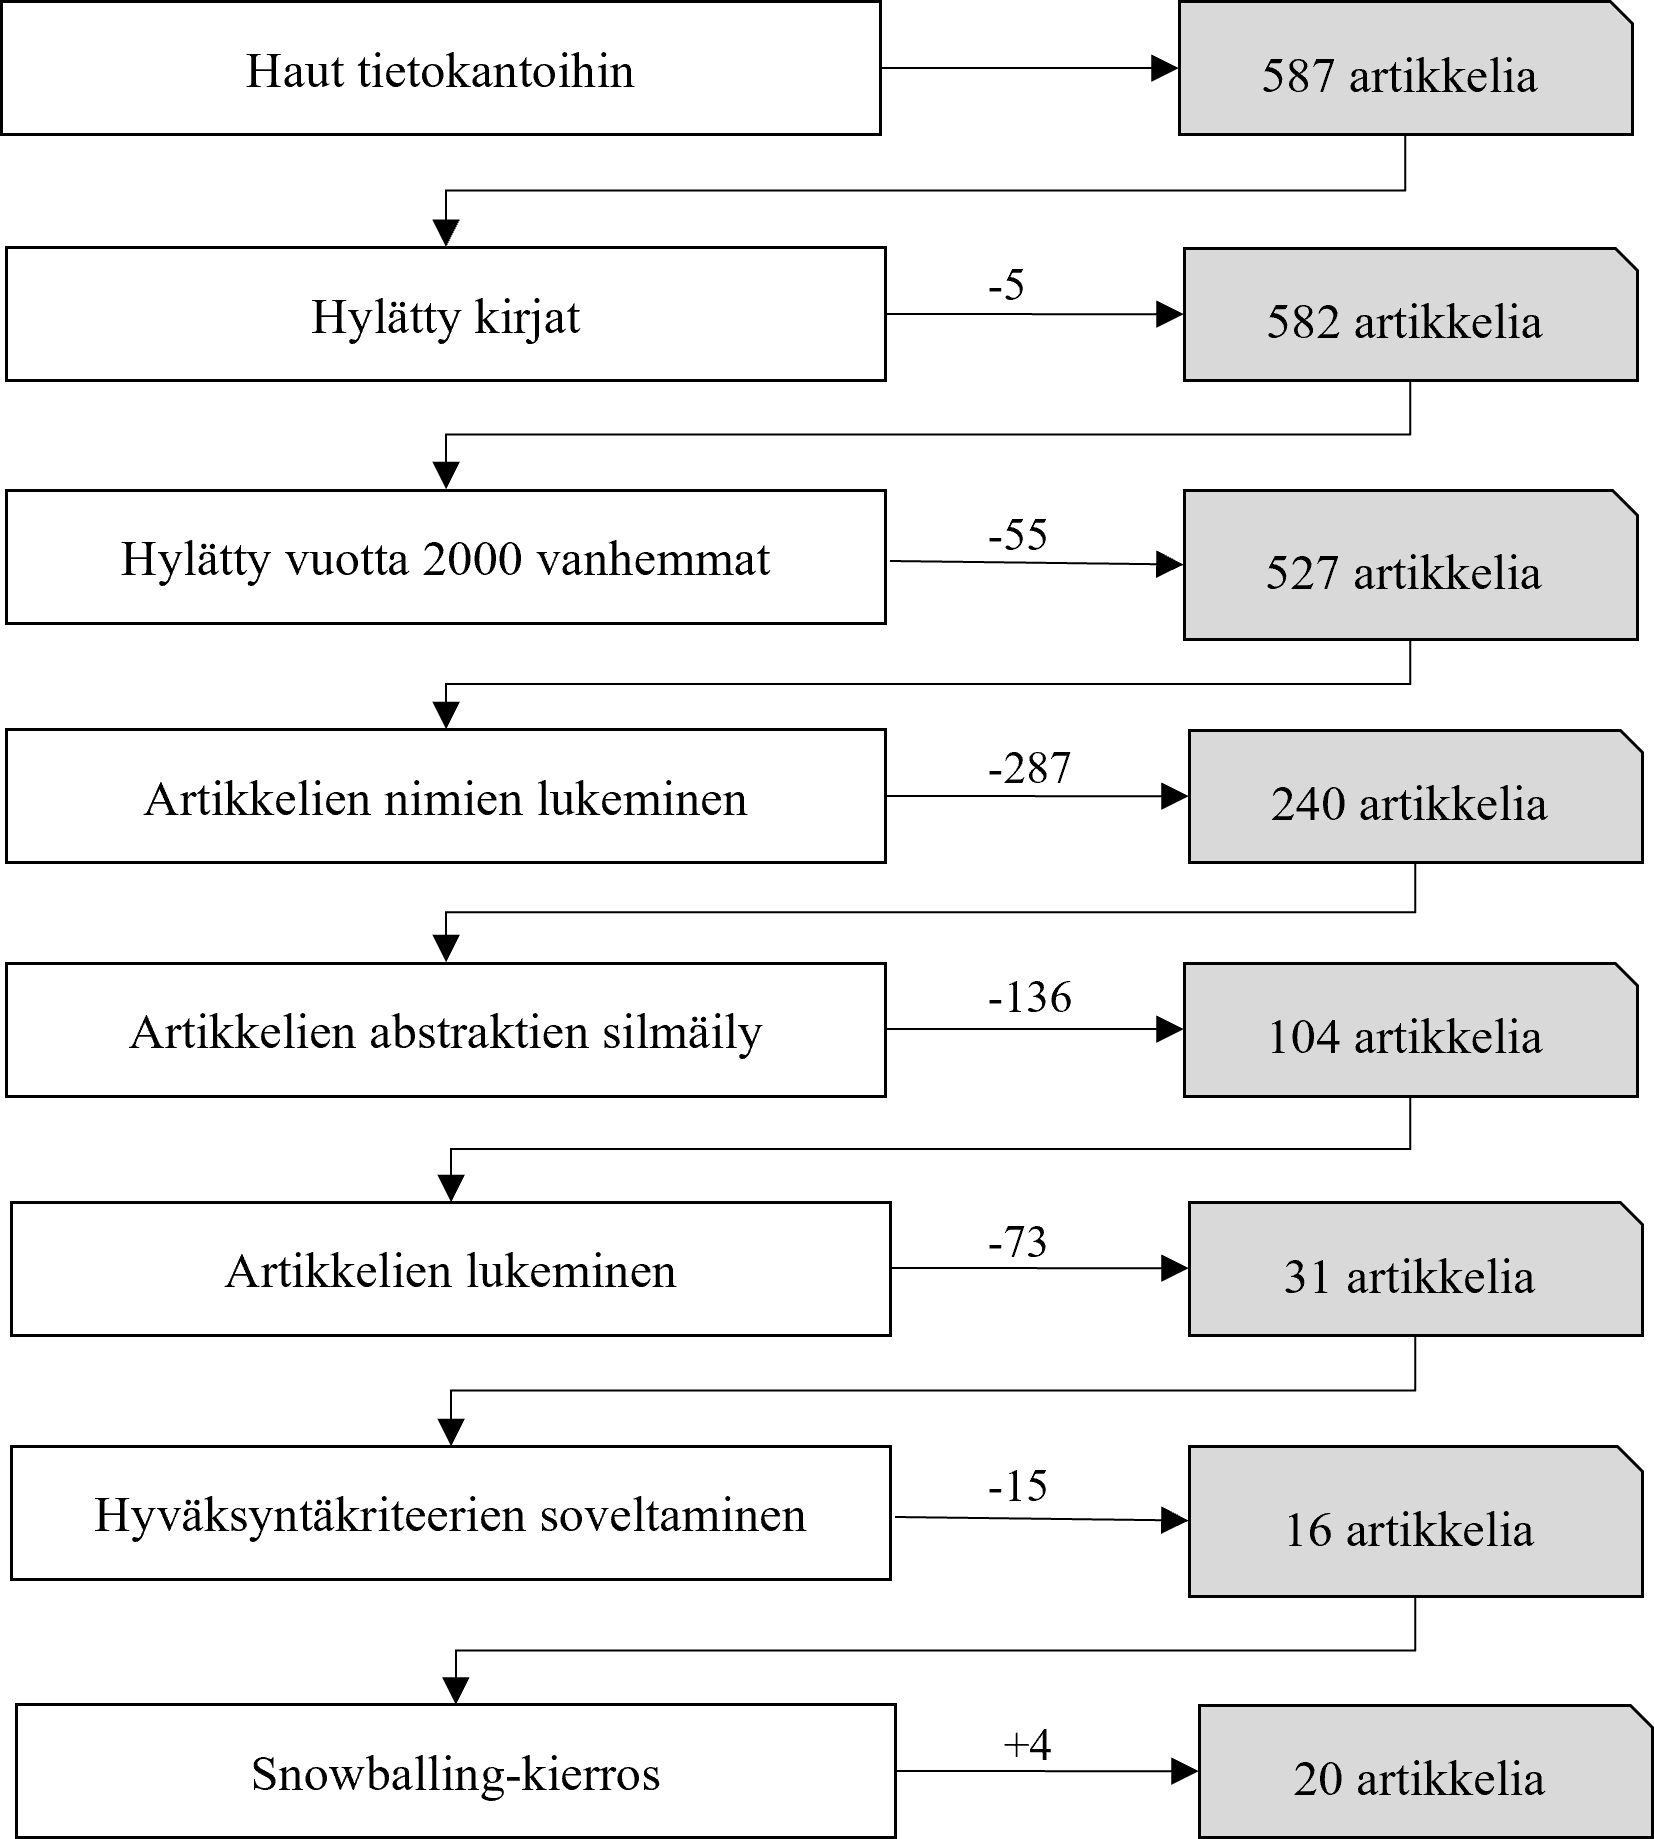
\includegraphics[width=11cm]{media/aineiston-rajaaminen-laaja-vaakalinja.png}
    \caption{Artikkelien valintamenettely}
    \label{kuvio:aineiston-rajaaminen-laaja}
\end{figure}

Yleisin artikkelin hylkäämiseen johtanut syy oli ``Muu aihe'', joka johti 422 artikkelin hylkäämiseen. Monissa artikkeleissa kontekstina oli avoimen lähdekoodin yhteisöjen perehdytyskäytännöt, mikä johti artikkelin hylkäämiseen. Neljässäkymmenessäviidessä artikkelissa taas käsiteltiin ohjelmistokehittäjien osaamista siltä kannalta, miten oppilaitokset voisivat parantaa opetussuunnitelmiaan vastaamaan yritysten tarpeita. Näissä näkökulmana oli siis oppilaitoksissa tehtävä työ, ei yritysten perehdytyskäytännöt. Useat artikkelit taas liittyivät yleisesti ohjelmistokehittäjien osaamisen parantamiseen, mutta ei nimenomaan perehdyttämisprosessin aikana. Monissa artikkeleissa esiteltiin tiedeyhteisön kehittämiä oivaltavia uusia työkaluja ja lähestymistapoja perehdyttämisen tukemiseen, mutta tässä tutkimuksessa pyrittiin tutkimaan nimenomaan organisaatioissa jo käytössä olevia käytäntöjä, joten nämä artikkelit hylättiin.

\section{Tiedonkeruustrategia}
\label{luku-tiedonkeruustrategia}

\textcite{kitchenham-charters-2007} mainitsevat, että tiedonkeruustrategia (engl. \textit{data extraction strategy}) määrittää sen, miten kustakin primääritutkimuksesta vaadittavat tiedot saadaan. Tämän tutkimuksen tiedonkeruustrategiaa tarkennettiin vaiheittain. Ensimmäinen versio strategiasta oli suuntaa-antava. Sitä pilotoitiin keräämällä dataa kolmesta potentiaalisesti katsaukseen soveltuvasta artikkelista. Pilotoinnin perusteella tiedonkeruustrategiaa täydennettiin merkittävästi lisäämällä siihen useita lisäkenttiä kuten tiedot tutkimuksen kohderyhmistä, tutkimuskohteen perehdyttämisen kontekstista ja tuloksista.

Seuraavaksi esitellään tiedonkeruustrategia kokonaisuudessaan. Aluksi jokaisesta artikkelista kerättiin lähdetietokannan tarjoama BibTex-tietue, joka sisälsi mm. seuraavat tiedot:

\begin{itemize}
    \item artikkelin nimi
    \item kirjoittajat
    \item DOI-osoite
    \item julkaisuvuosi
    \item abstrakti
\end{itemize}

Tietuetta täydennettiin seuraavilla tiedoilla:

\begin{itemize}
    \item hylkäyskriteeri
    \item jatkotutkimusaiheet
    \item tutkimuksen kohderyhmä
    \item perehdyttämisen konteksti
    \item tutkimuksen aineiston koko
    \item tutkimuksen kohdehenkilöiden työskentelymaa tai -alue
    \item artikkelissa mainitut perehdytyskäytännöt
    \item tiedonkeruun status (tiedot kerätty / kesken / ei kerätty)
    \item tutkimuksen tulokset
    \item tutkimusmenetelmät
    \item tutkimusasetelma
    \item ``twiitti'' eli lyhyt kuvaus tutkimuksesta
    \item valittu katsaukseen (kyllä / ei / ehkä)
    \item artikkelin rakenteeseen liittyviä tietoja (kuten onko tutkimuksen rajoituksia arvioitu) artikkelin laadun arvioimiseksi
\end{itemize}

\section{Tiedonkeruu ja tulkinta}

Artikkelien valitsemisen jälkeen suoritettiin tiedonkeruu, jossa artikkelit luettiin ja niistä kerättiin luvun \ref{luku-tiedonkeruustrategia} tiedonkeruustrategian mukaiset tiedot.

Tiedonkeruuvaiheessa pyrittiin tekemään mahdollisimman vähän tulkintaa, joten artikkeleista kerättiin vain sellainen tieto, jonka artikkelin kirjoittajat olivat eksplisiittisesti artikkelissa maininneet. Tavoitteena oli säilyttää data mahdollisimman autenttisena katsauksen laadun varmistamiseksi. Vasta kun tiedot oli kerätty kaikista artikkeleista, arvioitiin kerättyjä tietoja kokonaisuutena. Tämä johti joidenkin tietojen yhtenäistämiseen. Esimerkiksi eri artikkeleissa oli mainittu mentorointiin liittyviä käytäntöjä termeillä \textit{mentor}, \textit{buddy} ja \textit{tutor}. Datassa nämä yhtenäistettiin käytännön \textit{mentorointi} alle. Eri artikkeleissa oli mainittu myös tulokkaan perehtyminen yrityksen sisäiseen intranettiin, wikiin tai muuhun vastaavaan tietovarastoon. Nämä käytännöt yhtenäistettiin käsitteellä \textit{sisäiseen dokumentaatioon perehtyminen}.

Myös muita kerättyjä tietoja yhtenäistettiin ja selkeytettiin. Esimerkiksi \textit{juniorit} saattoi olla merkitty sekä kontekstiksi että kohderyhmäksi tai \textit{katselmointi} sekä kontekstiksi että perehdytyskäytännöksi. Näissä tilanteissa tiedot yhdenmukaistettiin.

Käsitteellisesti toisiaan muistuttavien tietojen eroja tulkittiin joko yhdistämällä kaksi käsitettä (kyselytutkimusten osalta tutkimusmenetelmäksi merkitty \textit{avoimet kysymykset} yleistettiin \textit{kysely}-menetelmän alle) tai tulkitsemalla käsitteiden eroja: kontekstien \textit{etätyöskentely} ja \textit{globaalisti hajautettu ohjelmistokehitys} eroiksi tulkittiin se, että jälkimmäisessä hajauttaminen on tehty tarkoituksella ja etätyöskentelyssä olosuhteiden pakosta. Etätyöskentely toki voi olla vapaaehtoistakin, mutta tämän katsauksen artikkeleissa sitä tehtiin pandemiaan \parencite{rodeghero-ym-2021} tai työlupiin \parencite{hemphill-begel-2011} liittyvien rajoitteiden vuoksi. \textcite{britto-ym-2020} tutkivat Ericsson AB:lle palkattujen intialaisten ja \textcite{moe-ym-2020} norjalaiseen pankkiin palkattujen portugalilaisten ohjelmistokehittäjien käytäntöjä - näissä kontekstiksi merkittiin \textit{globaalisti hajautettu ohjelmistokehitys}.

\chapter{Tulokset}
\label{paaluku-tulokset}

TODO metateksti

\section{Katsaukseen valitut artikkelit}

Tähän systemaattiseen kirjallisuuskatsaukseen valittiin siis yhteensä 20 artikkelia. Artikkelit on esitelty taulukossa \ref{tbl:artikkelit}. Niissä käsitellään perehdyttämistä eri näkökulmista. Esimerkiksi \textcite{johnson-senges-2010} kertovat Googlen ohjelmistokehittäjien perehdytyskäytännöistä, \textcite{britto-ym-2020} käsittelevät aihetta globaalisti hajautetussa ohjelmistokehityksessä ja \textcite{bjornson-dingsøyr-2005} pienessä konsulttiyrityksessä. Artikkelit on julkaistu vuosina 2005-–2021. Valtaosa artikkeleista, viisitoista kappaletta, on julkaistu vuoden 2015 jälkeen. Tarkat kappalemäärät julkaisuvuosittain on esitelty kuviossa \ref{kuvio:kappalemaarat-julkaisuvuosittain-tiivis}. Yhdysvalloista mukana oli kahdeksan tutkimusta, Intiasta neljä ja Kanadasta kolme (ks. kuvio \ref{kuvio:maat}).

\begin{figure}[h]
    \centering
    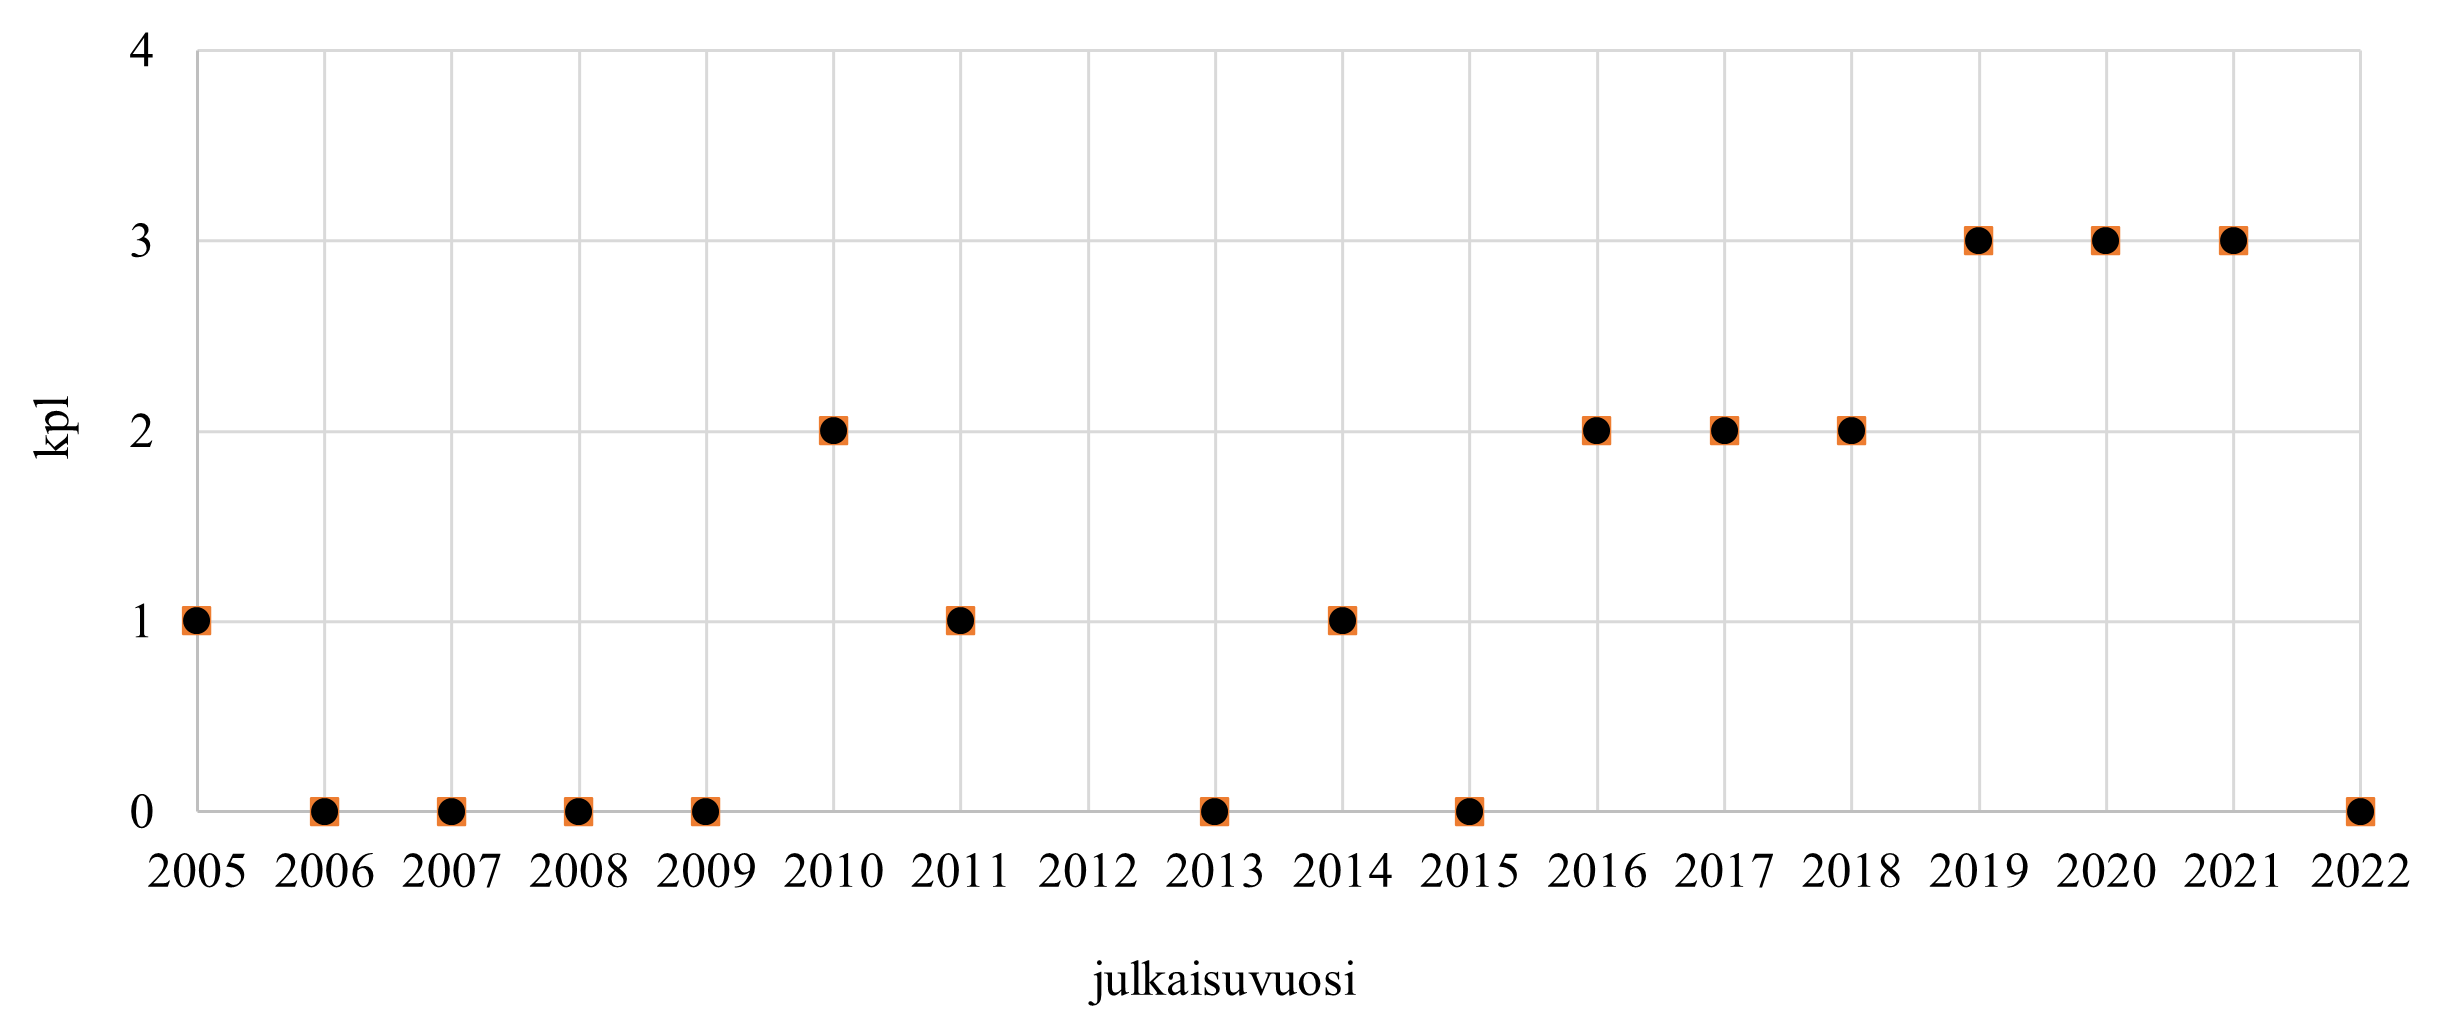
\includegraphics[width=\textwidth]{media/kappalemaarat-julkaisuvuosittain-tiivis.png}
    \caption{Artikkeleiden kappalemäärät julkaisuvuosittain}
    \label{kuvio:kappalemaarat-julkaisuvuosittain-tiivis}
\end{figure}

\begin{figure}[h]
    \centering
    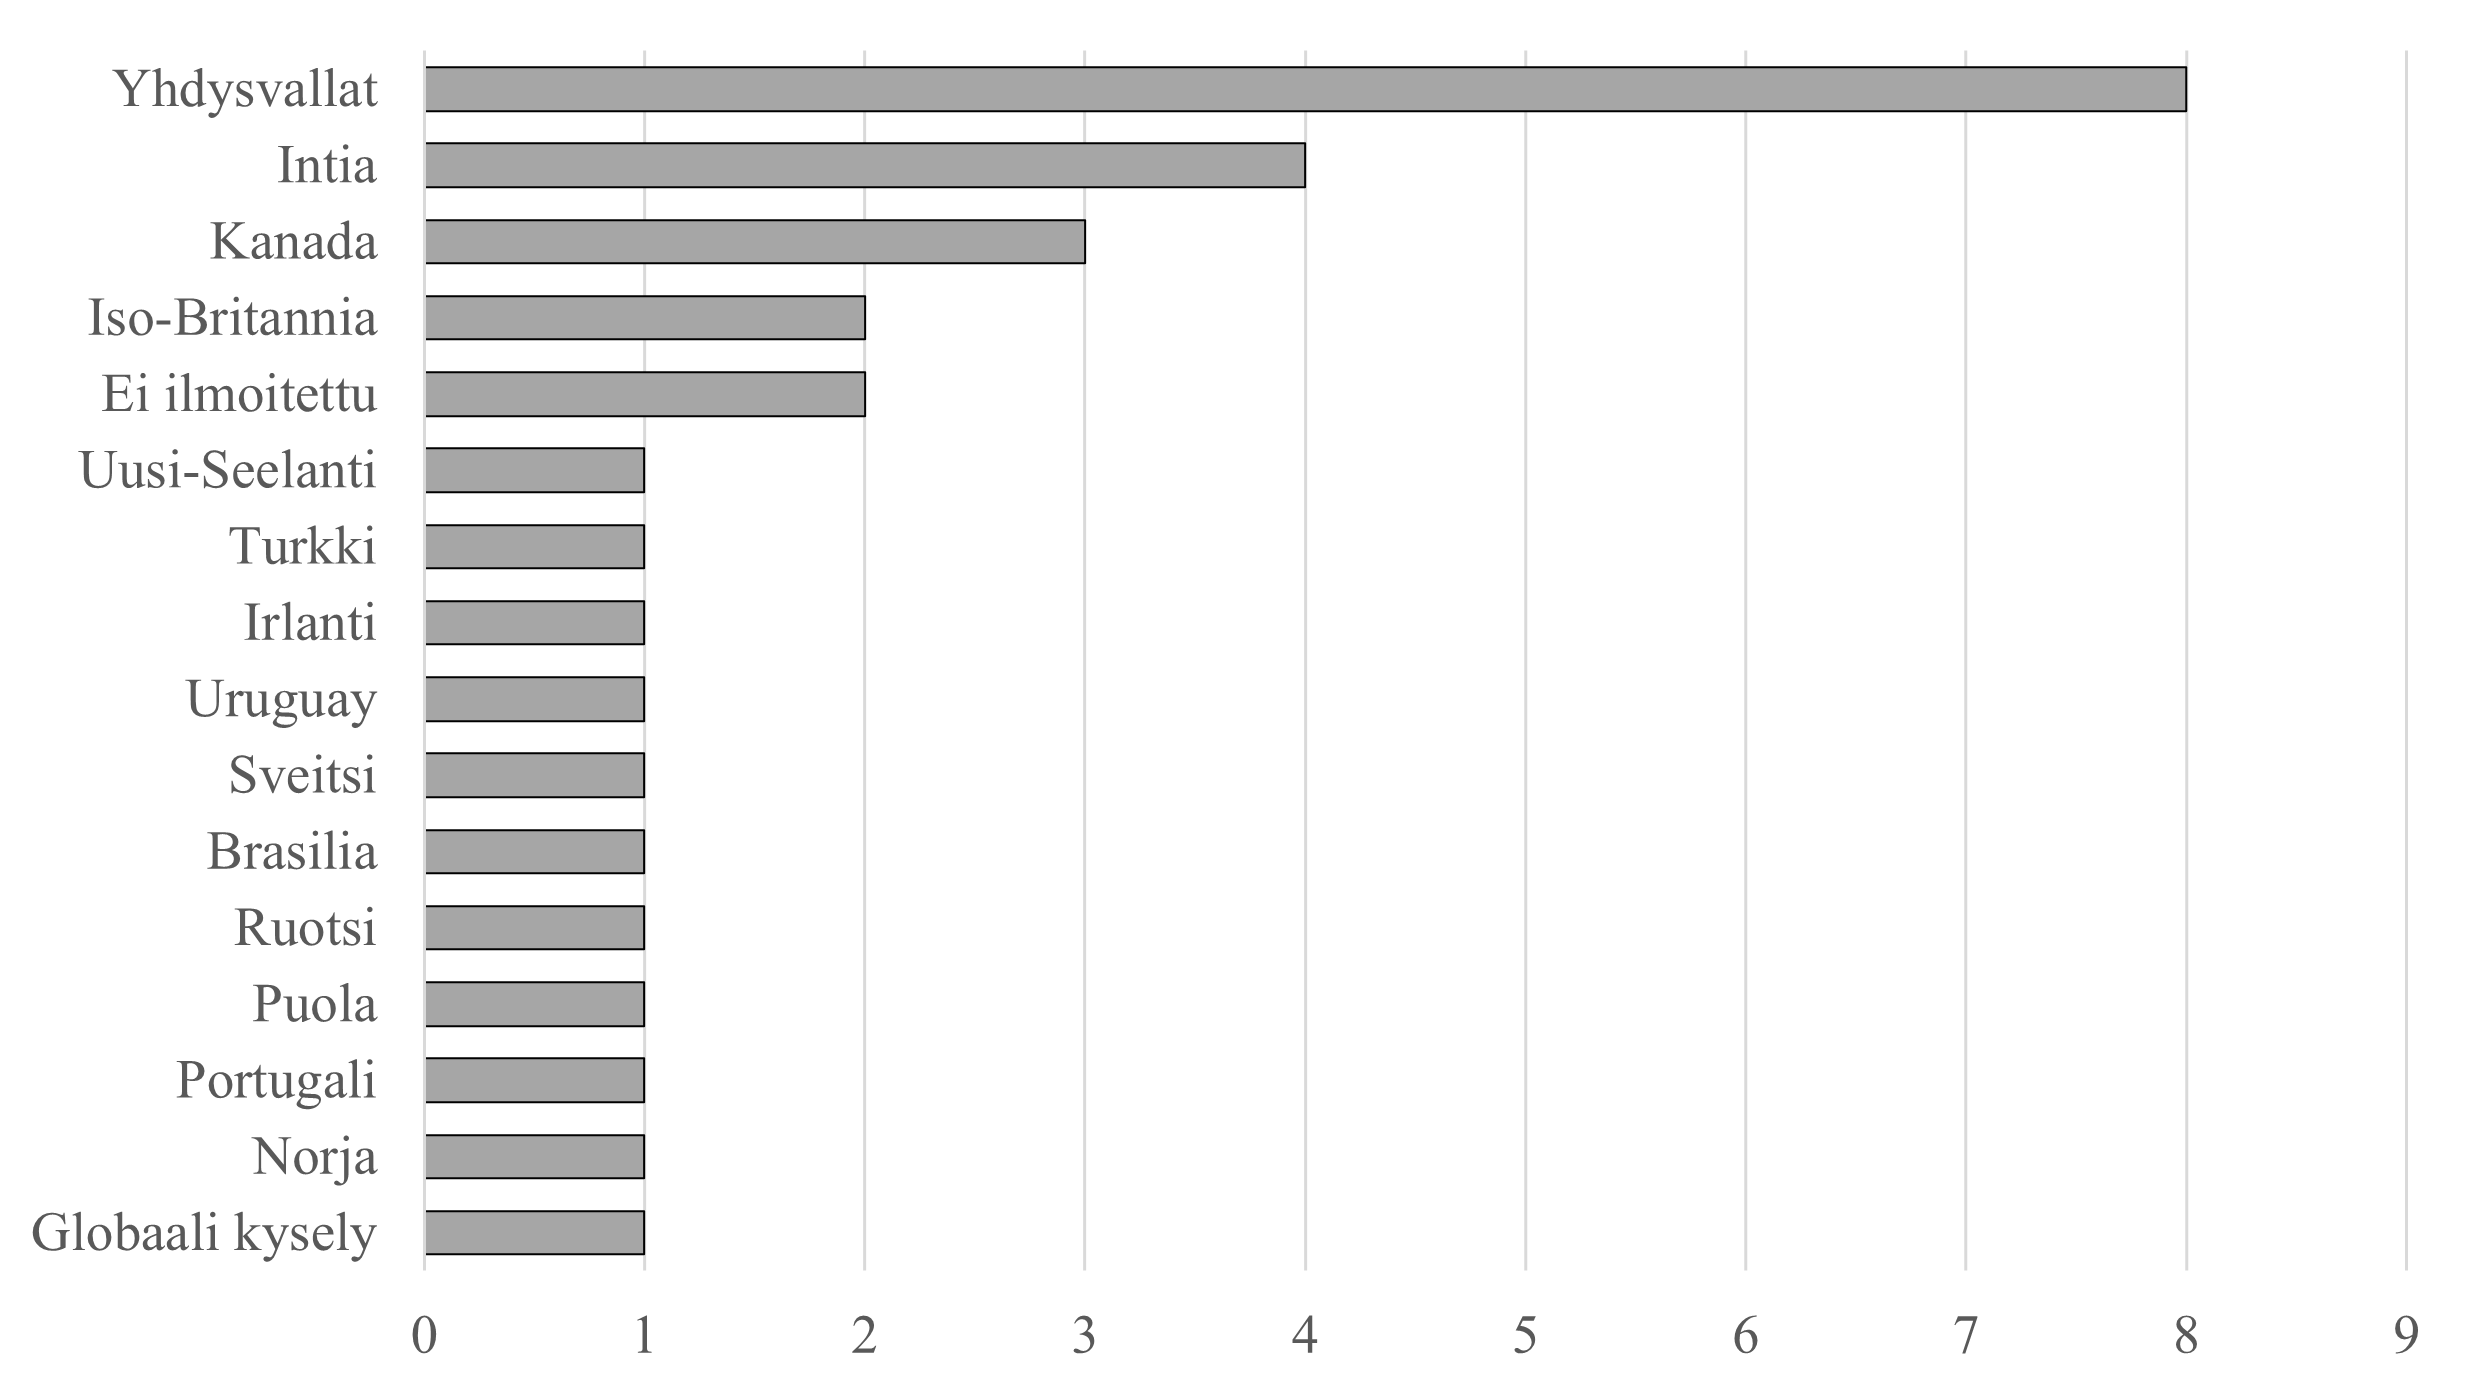
\includegraphics[width=\textwidth]{media/maat.png}
    \caption{Tutkimuskohteiden työskentelymaat}
    \label{kuvio:maat}
\end{figure}

Artikkeleista kuusi oli ilmestynyt tietojenkäsittelytieteen alan journal-lehdissä. Kolmetoista artikkelia taas oli julkaistu tieteellisten konferenssien kokoomateoksissa (engl. \textit{proceedings}). Yksi artikkeli \parencite{hemphill-begel-2011} on ilmestynyt Microsoft Technical Report -julkaisusarjassa. Tämä artikkeli havaittiin snowballing-kierroksen aikana. Sitä ei ole ole julkaistu tieteellisessä julkaisussa, mutta kirjoittajiensa tieteellisten ansioiden vuoksi sen sisällyttämistä katsaukseen arvioitiin silti. Artikkelin todettiin tuovan merkittävää tietoa perehdyttämisestä virtuaalisissa tiimeissä, mikä on erityisen oleellista etätyön lisäännyttyä, joten artikkeli sisällytettiin katsaukseen.

Tutkimusten lähdeaineistojen koko eli datapisteiden määrä vaihteli kolmen \parencite{kulkarni-ym-2010} ja 267 datapisteen \parencite{rodeghero-ym-2021} välillä, keskiarvon ollessa 45. Yhteensä katsauksen artikkeleissa oli 765 datapistettä eli haastateltua henkilöä, kyselyyn vastaajaa tai yhdessä tutkimuksessa myös havainnoitua perehdytyssessiota. Sessio, johon osallistui useita henkilöitä, on tässä siis laskettu yhdeksi datapisteeksi. Sessioita havainnoitiin vain yhdessä tutkimuksessa. 

\begin{footnotesize}
    \begin{longtable}{ m{4cm}  m{10.5cm} }
    \hline
        \hline
           \textbf{Tekijä(t) ja vuosi} & \textbf{Artikkelin nimi} \\
        \hline
    \endfirsthead

    \hline
        \hline
           \textbf{Tekijä(t) ja vuosi} & \textbf{Artikkelin nimi} \\
        \hline
    \endhead
 \hline
 \endfoot

 \caption{Artikkelit \label{tbl:artikkelit}}
 \endlastfoot

\textcite{rodeghero-ym-2021} & Please Turn Your Cameras On: Remote Onboarding of Software Developers during a Pandemic \\
\hline
\textcite{azanza-ym-2021} & Onboarding in Software Product Lines: Concept Maps as Welcome Guides \\
\hline
\textcite{ju-ym-2021} & A Case Study of Onboarding in Software Teams: Tasks and Strategies \\
\hline
\textcite{britto-ym-2020} & Evaluating and strategizing the onboarding of software developers in large-scale globally distributed projects\\
\hline
\textcite{yates-ym-2020} & Characterizing the transfer of program comprehension in onboarding: an information-push perspective\\
\hline
\textcite{moe-ym-2020} & Studying Onboarding in Distributed Software Teams: A Case Study and Guidelines \\
\hline
\textcite{kumar-wallace-2019} & Patterns of Identity and Interaction in an Agile Community of Practice \\
\hline
\textcite{viviani-murphy-2019} & Reflections on Onboarding Practices in Mid-Sized Companies \\
\hline
\textcite{buchan-ym-2019} & Effective team onboarding in Agile software development: techniques and goals \\
\hline
\textcite{tuzun-ym-2018} & Are computer science and engineering graduates ready for the software industry? Experiences from an industrial student training program \\
\hline
\textcite{matturro-ym-2017} & Difficulties of Newcomers Joining Software Projects Already in Execution \\
\hline
\textcite{britto-ym-2017} & Onboarding software developers and teams in three globally distributed legacy projects: A multi-case study \\
\hline
\textcite{pham-ym-2017} & Onboarding inexperienced developers: struggles and perceptions regarding automated testing \\
\hline
\textcite{kumar-ym-2016} & Mentoring trajectories in an evolving agile workplace \\
\hline
\textcite{shannon-pool-2016} & Agile Processes, in Software Engineering, and Extreme Programming \\
\hline
\textcite{viana-ym-2014} & Knowledge transfer between senior and novice software engineers: A qualitative analysis \\
\hline
\textcite{hemphill-begel-2011} & Not Seen and Not Heard: Onboarding Challenges in Newly Virtual Teams \\
\hline
\textcite{kulkarni-ym-2010} & From Student to Software Engineer in the Indian IT Industry: A Survey of Training \\
\hline
 \textcite{johnson-senges-2010} & Learning to be a programmer in a complex organization: A case study on practice-based learning during the onboarding process at Google\\
\hline
\textcite{bjornson-dingsøyr-2005} & A Study of a Mentoring Program for Knowledge Transfer in a Small Software Consultancy Company \\

\hline
\end{longtable}
\end{footnotesize}


\section{Perehdytyskäytännöt}
\label{luku-tulokset-kaytannot}

Artikkeleissa mainittiin yhteensä 45 erilaista perehdytyskäytäntöä, jotka esitellään esiintymismäärineen kuviossa \ref{kuvio:kaytannot}. Mentorin nimeäminen oli yleisin, sillä se mainittiin kuudessatoista artikkelissa tulokkaiden perehdytyskäytäntönä. Ohjelmakoodin katselmointi (engl. \textit{code review}) mainittiin yhdeksässä artikkelissa, kuten myös yhteistoiminnallinen ohjelmointi (pari- tai ryhmäohjelmointi). Organisaation sisäiseen dokumentaatioon perehtyminen oli kirjattu käytännöksi seitsemään eri artikkeliin. Tulokkaiden toiminta vertaisryhmänä, työtehtävän kontekstualisointi ja erilaiset tarkistuslistat saivat kukin viisi mainintaa, kuten myös ``Good First Issue'', joka viittaa työtehtävään, joka on ennakolta määritelty tulokkaalle erityisen hyvin sopivaksi.

\begin{figure}[h]
    \centering
    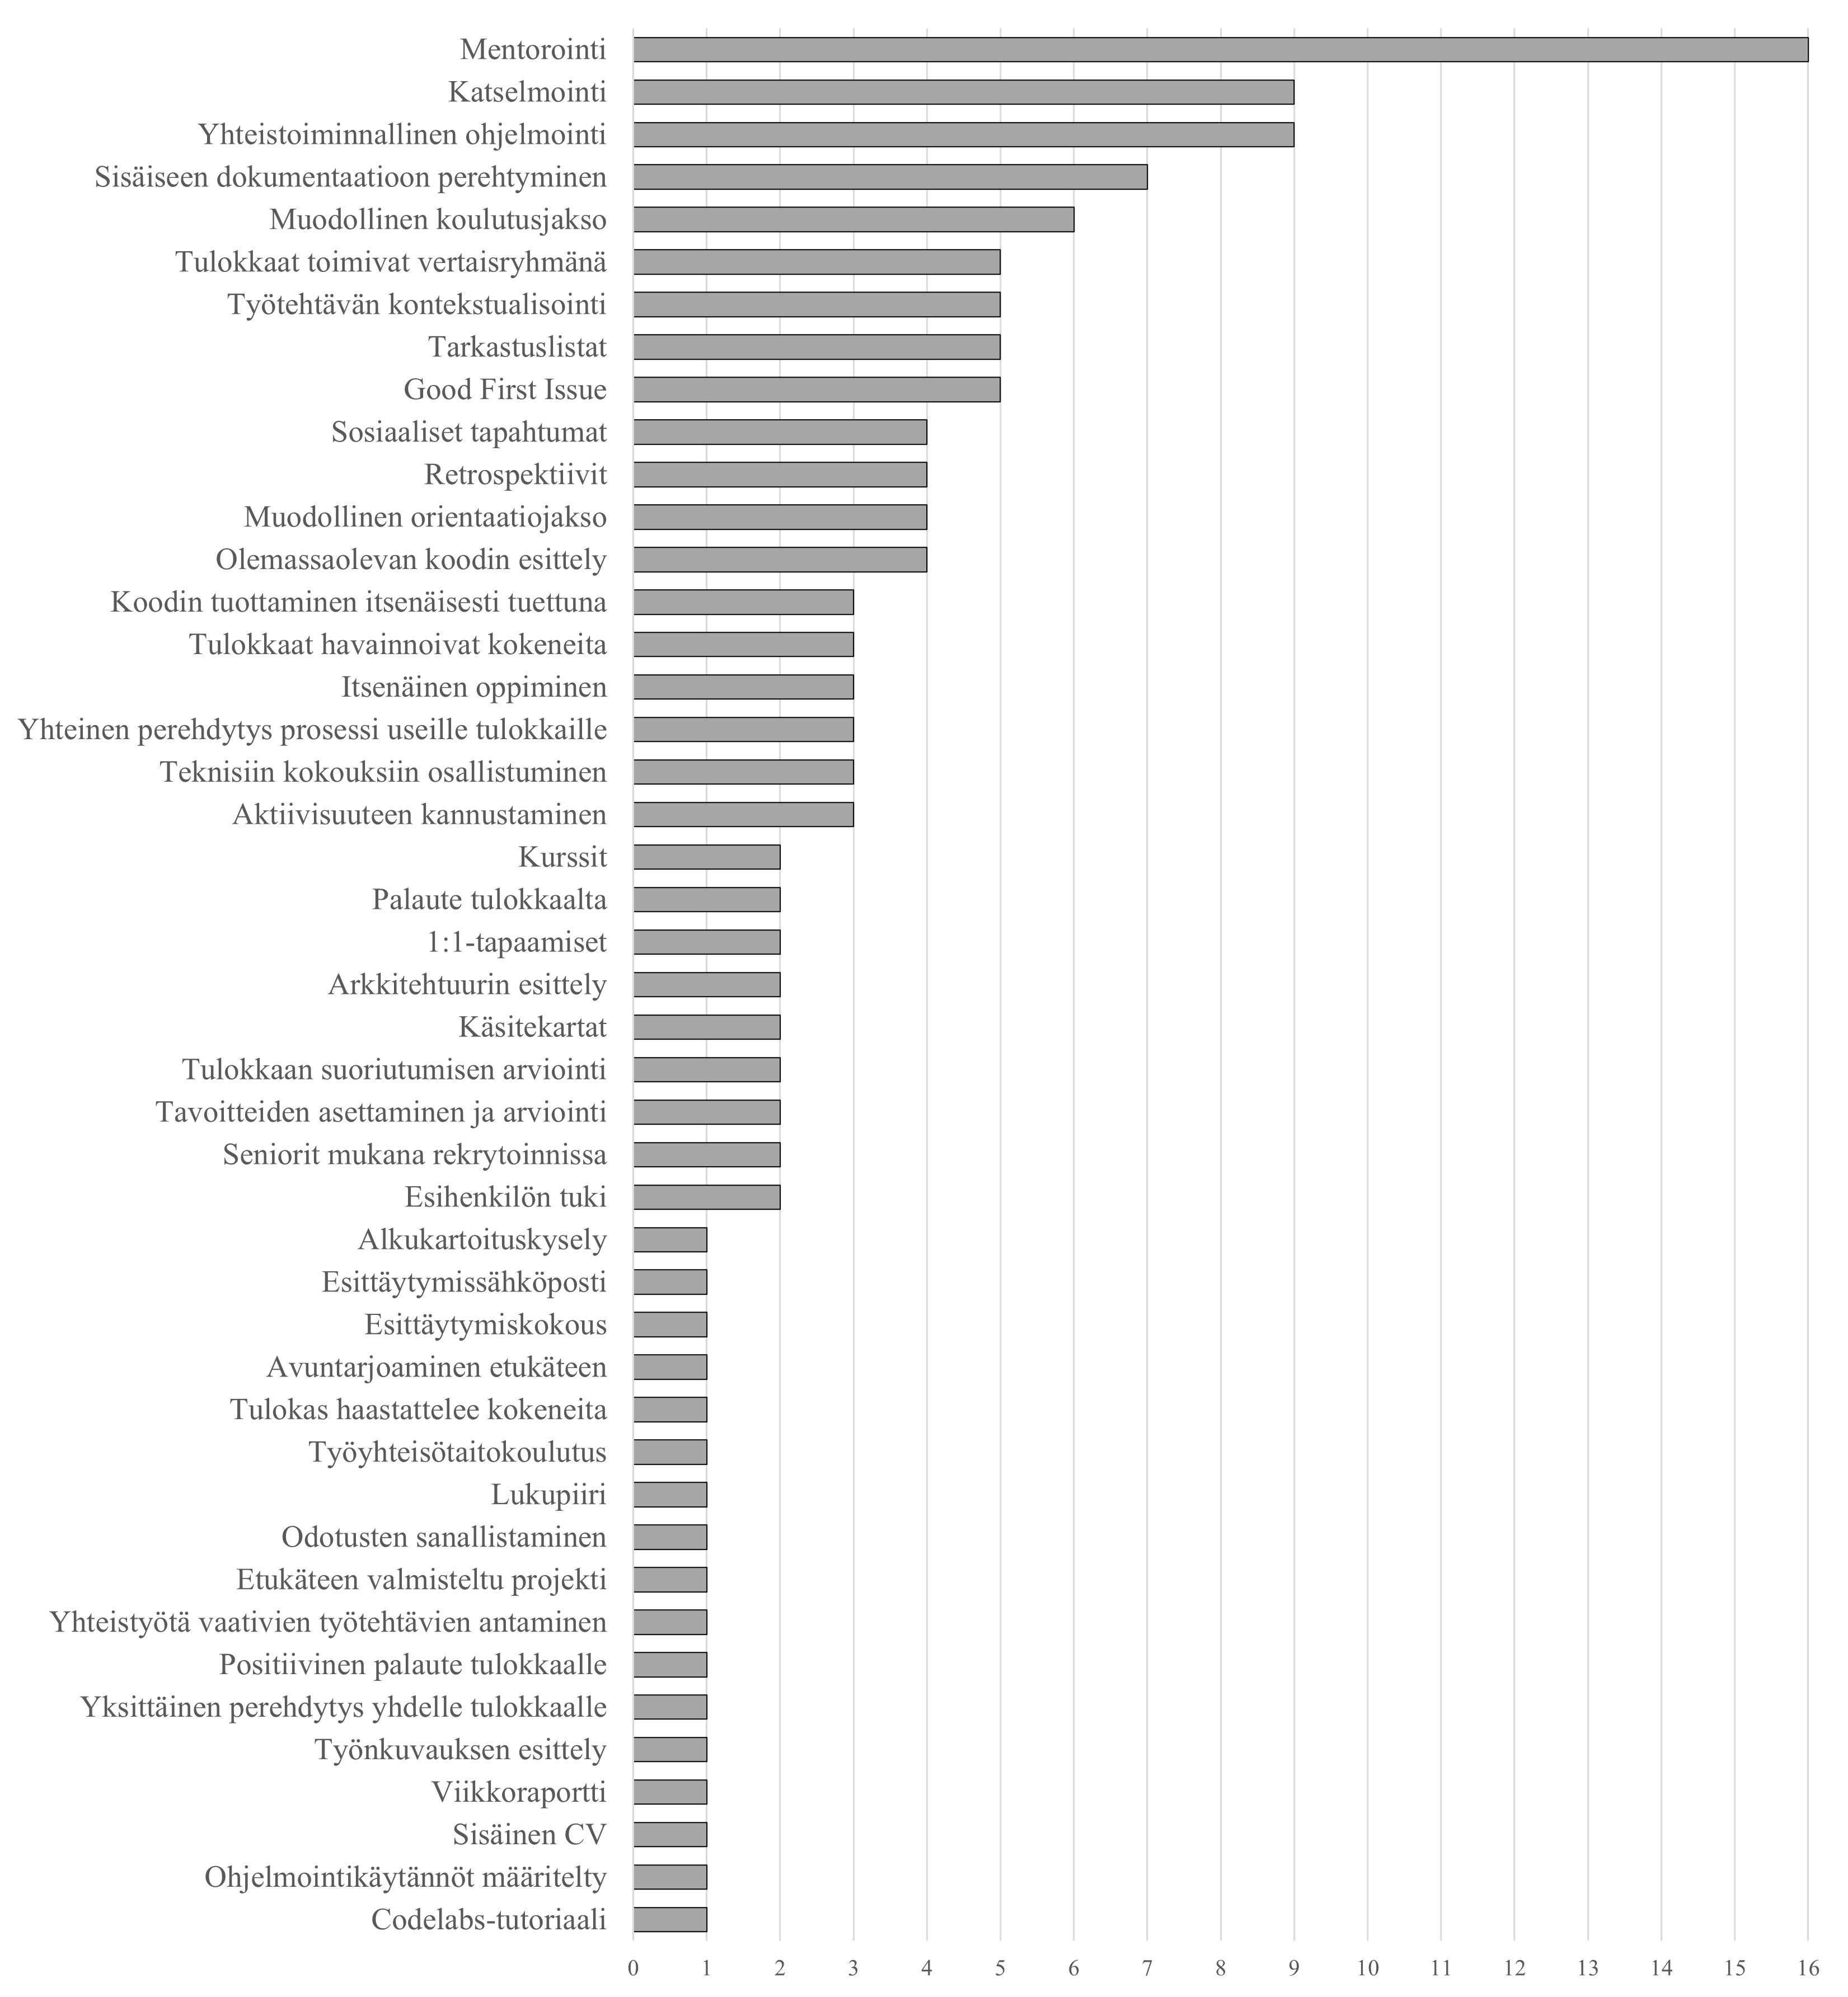
\includegraphics[width=13.25cm]{media/45-kaytannot.png}
    \caption{Perehdyttämiskäytäntöjen esiintymismäärät}
    \label{kuvio:kaytannot}
\end{figure}

Artikkeleissa mainitut perehdyttämiskäytännöt jaoteltiin luvussa \ref{luku-SRT-teoria} esitellyn sosialisaatioresurssien teorian mukaisesti. Jaottelu on havainnollistettu taulukossa \ref{tbl:longtable-srt-ulottuvuudet-ja-niiden-kaytannot}. Esimerkiksi sosialisaatioresurssien teorian ennakoivaan sosialisaatioon (ulottuvuus 1) sijoitettiin alkukartoituskyselyihin ja esittäytymissähköposteihin liittyvät käytännöt. Ulottuvuuksien mainintamäärät on kuvattu kuviossa \ref{kuvio:ulottuvuudet}. Mentorointi (ulottuvuus 4) oli yleisin, sillä se mainittiin 16 artikkelissa. Viidessätoista artikkelissa mainittiin käytännön työtehtäviin ja työn luonteeseen liittyviä käytäntöjä (ulottuvuus 12). Näitä olivat esimerkiksi työtehtävän kontekstualisointi, ``Good First Issue'' ja yhteistoiminnallinen ohjelmointi. Seuraavaksi eniten mainintoja sai palautteen ulottuvuus (11 artikkelia), johon luettiin katselmointi, tulokkaalle annettava positiivinen palaute ja tulokkaan suoriutumisen arviointi.

\setlength{\LTcapwidth}{\textwidth}
 \begin{scriptsize}
        \begin{longtable}[c]{llll}
        \multicolumn{4}{c}{}\\
            \hline
                \textbf{Nro} & \textbf{Ulottuvuus} \parencite{saks-gruman-2012} & \textbf{Katsauksessa mainittu perehdytyskäytäntö} & \textbf{Mainintojen määrä} \\
            \hline
        \endfirsthead
        \hline
            \hline
                \textbf{Nro} & \textbf{Ulottuvuus} \parencite{saks-gruman-2012} & \textbf{Katsauksessa mainittu perehdytyskäytäntö} & \textbf{Mainintojen määrä} \\
            \hline
        \endhead
     \hline
     \endfoot
    \caption{Artikkeleissa havaitut perehdytyskäytännöt sosialisaatioresurssien teoriaan \parencite{saks-gruman-2012} pohjautuen jaoteltuna \label{tbl:longtable-srt-ulottuvuudet-ja-niiden-kaytannot}}
    \endlastfoot
    
    1 & Ennakoiva sosialisaatio & Alkukartoituskysely & 1 \\
    & & Esittäytymissähköposti & 1 \\
    \hline
    2 & Muodollinen orientaatiojakso & Muodollinen orientaatiojakso & 4\\
    \hline
    3 & Oma-aloitteisuuteen kannustaminen & Aktiivisuuteen kannustaminen & 3 \\
    & & Tulokas haastattelee kokeneita & 1 \\
    \hline
    4 & Mentorointi & Mentorointi & 16 \\
    \hline
    5 & Sosiaaliset tapahtumat & Esittäytymiskokous & 1 \\
    & & Sosiaaliset tapahtumat & 4\\
    \hline
    6 & Sosialisaatioagentit & Avun tarjoaminen etukäteen & 1 \\
    \hline
    7 & Esihenkilön tuki & Esihenkilön tuki & 2 \\
    & & 1:1-tapaamiset & 2 \\
    \hline
    9 & Työn tekemisen resurssit & Sisäiseen dokumentaatioon perehtyminen & 7 \\
    & & Ohjelmointikäytännöt määritelty & 1 \\
    \hline
    10 & Työn suunnittelu & Tarkastuslistat & 5\\
    & & Odotusten sanallistaminen & 1 \\
    & & Tavoitteiden asettaminen ja arviointi & 2\\
    \hline
    11 & Muodollinen työnopetus & Kurssit & 2 \\
    & & Muodollinen koulutusjakso & 6 \\
    & & Työyhteisötaitokoulutus & 1\\
    & & Codelabs-tutoriaali & 1\\
    \hline
    12 & Työtehtävät ja työn luonne & Työtehtävän kontekstualisointi & 5 \\
    & & Good First Issue & 5 \\
    & & Etukäteen valmisteltu projekti & 1 \\
    & & Viikkoraportti & 1 \\
    & & Koodin tuottaminen itsenäisesti tuettuna & 3\\
    & & Teknisiin kokouksiin osallistuminen & 3\\
    & & Retrospektiivit & 4\\
    & & Yhteistoiminnallinen ohjelmointi & 9\\
    \hline
    13 & Informaatio & Työnkuvauksen esittely & 1\\
    & & Arkkitehtuurin esittely & 2\\
    & & Käsitekartat & 2\\
    & & Olemassaolevan koodin esittely & 4\\
    \hline
    14 & Palaute & Katselmointi & 9\\
    & & Positiivinen palaute tulokkaalle & 1\\
    & & Tulokkaan suoriutumisen arviointi & 2\\
    \hline
    17 & Perehdytysprosessin arviointi & Palaute tulokkaalta & 2\\
    \hline
    18 & Orientaation jälk. tulokkaiden keskinäinen oppiminen & Tulokkaat toimivat vertaisryhmänä & 5\\
    & & Yhteistyötä vaativien työtehtävien antaminen & 1\\
    & & Yhteinen perehdytysprosessi useille tulokkaille & 3\\
    & & Lukupiiri & 1\\
    \hline
    & Ei luokiteltavissa & Sisäinen CV & 1 \\
    & & Tulokkaat havainnoivat kokeneita & 3\\
    & & Seniorit mukana rekrytoinnissa & 2\\
    & & Yksittäinen perehdytys yhdelle tulokkaalle & 1\\
    & & Itsenäinen oppiminen & 3\\
    \hline
    
    \end{longtable}
    \end{scriptsize}

Neljä perehdytyskäytäntöä liittyi selvästi orientaatiovaiheen jälkeiseen tulokkaisen keskinäiseen yhteistoiminnalliseen oppimiseen. Näissä käytännöissä samaan aikaan organisaatioon liittyneet tulokkaat toimivat siis yhdessä. Heille saatettiin antaa yhteistyötä vaativia työtehtäviä. Eräässä organisaatiossa yksi perehdytyskäytännöistä oli lukupiiri, jossa käsiteltiin ohjelmistokehitykseen liittyviä artikkeleita. Nämä yhteistoiminnallista oppimista edistävät käytännöt on tässä sijoitettu ulottuvuuteen 18, joka täydentää sosialisaatioresurssien teorian aiempia ulottuvuuksia. Kuten kuviosta \ref{kuvio:ulottuvuudet} nähdään, tämä ulottuvuus on saanut neljänneksi eniten mainintoja kaikista ulottuvuuksista. Siihen kuuluvia käytäntöjä on mainittu yhdeksässä artikkelissa. 

\begin{figure}[h]
    \centering
    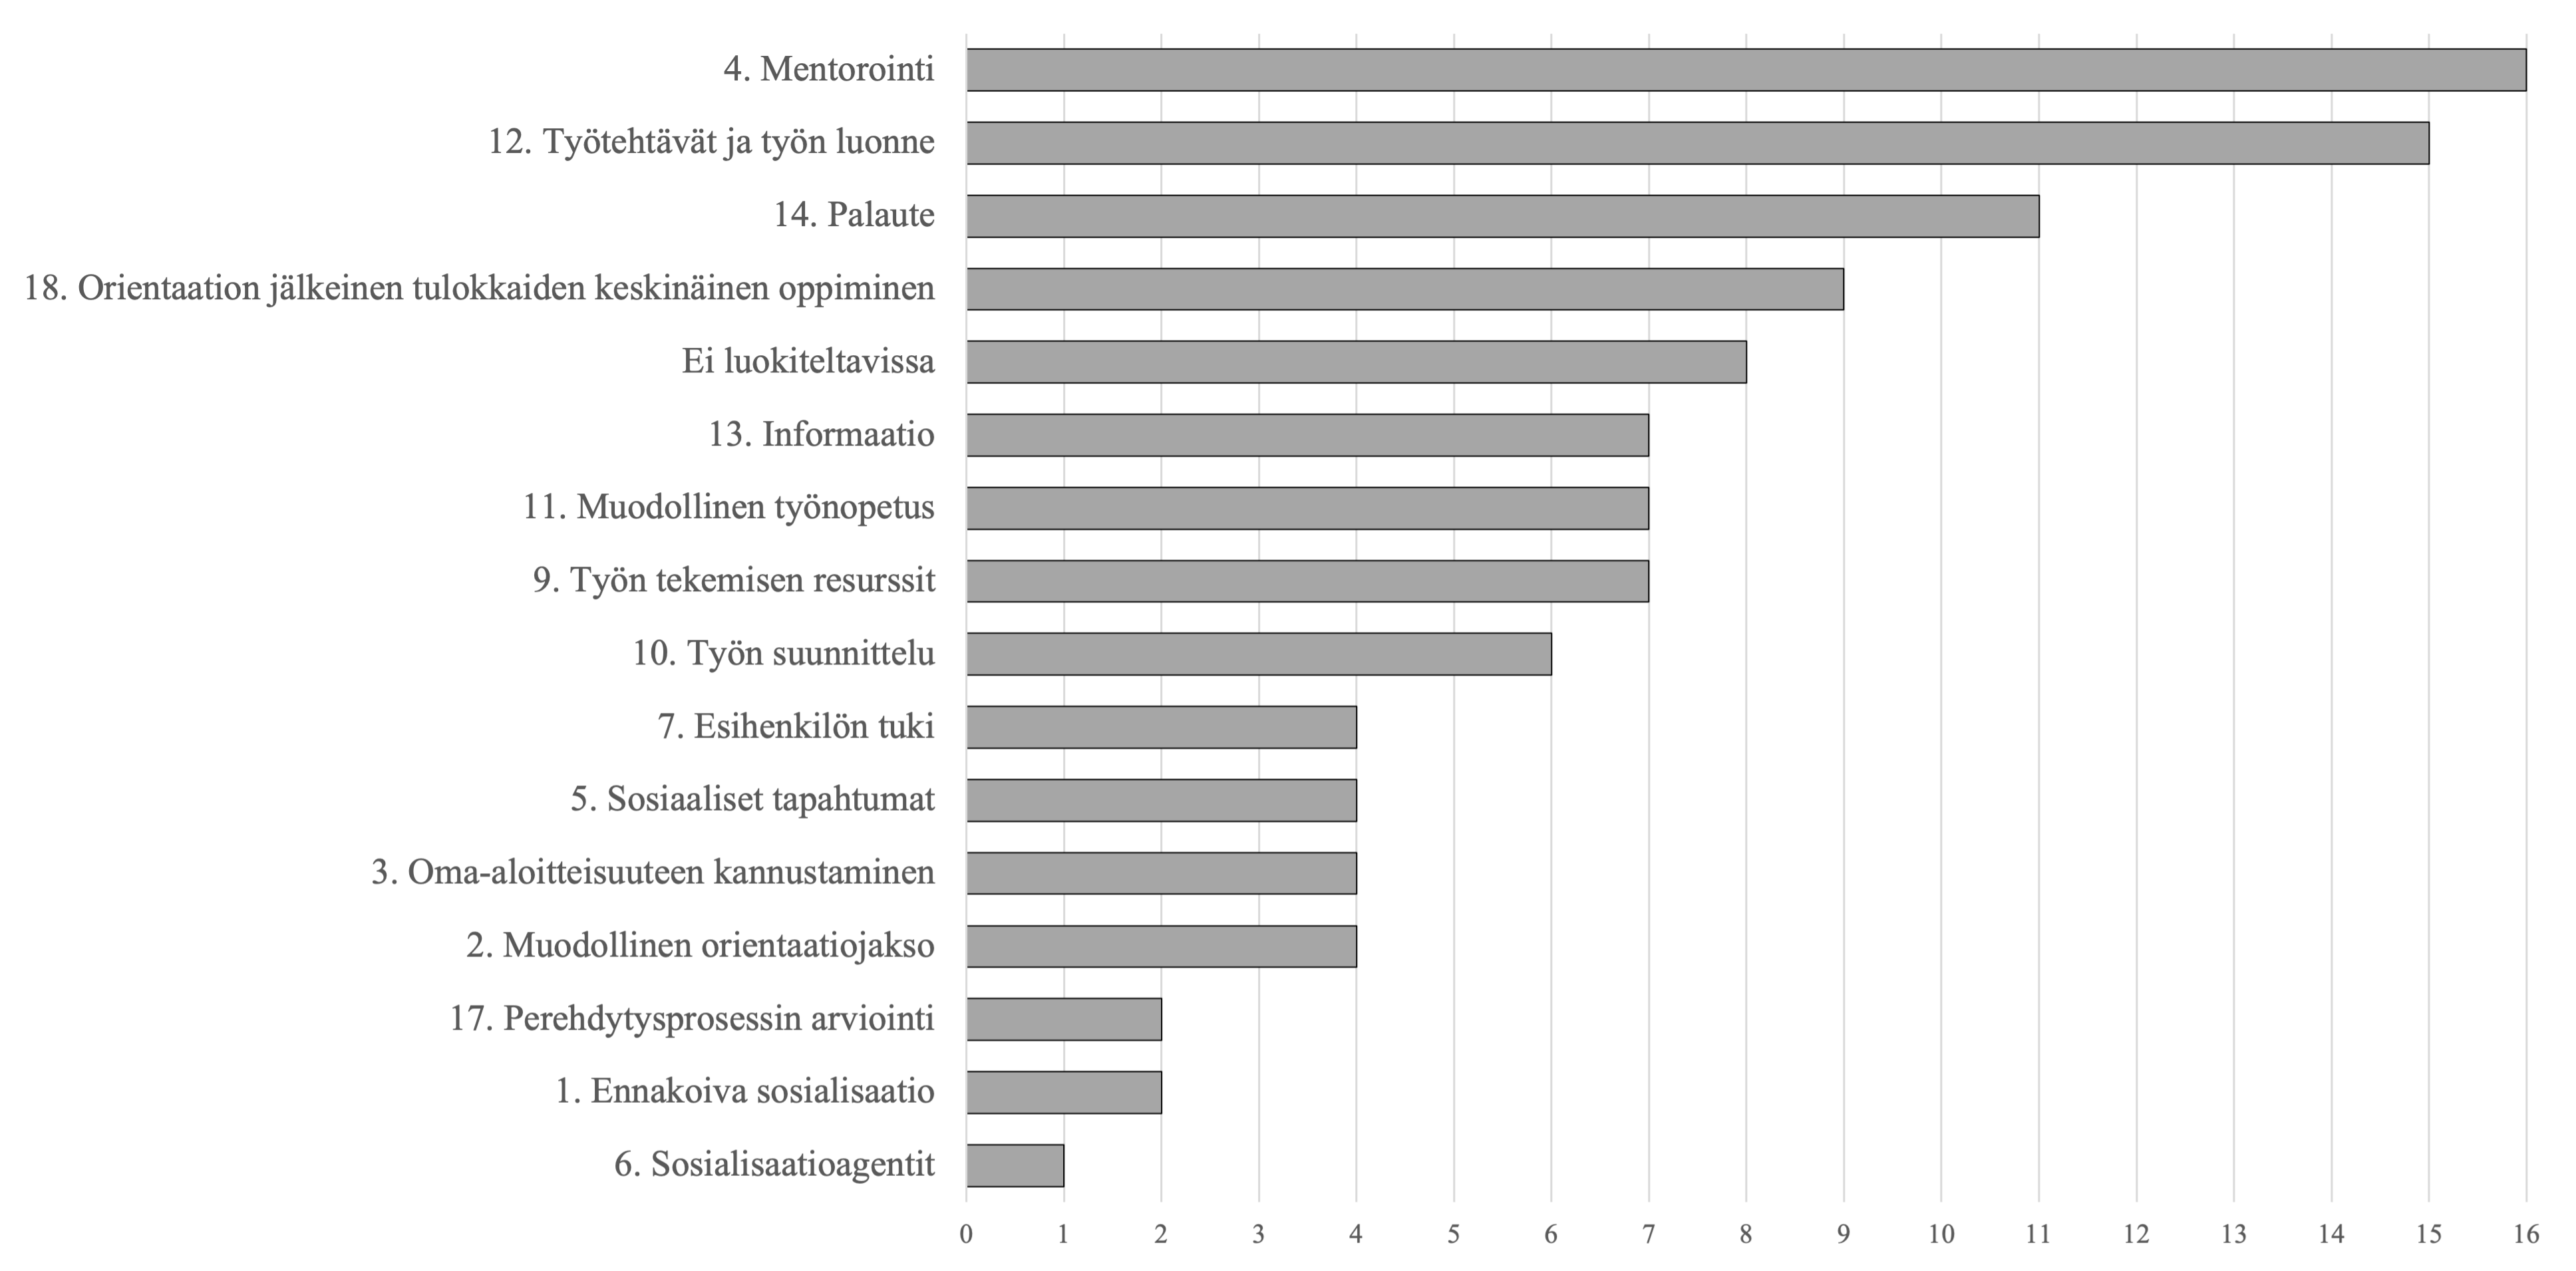
\includegraphics[width=\textwidth]{media/ulottuvuudet.png}
    \caption{Perehdyttämiskäytäntöjen esiintymismäärät jaoteltuna sosialisaatioresurssien \parencite{saks-gruman-2012} ulottuvuuksien mukaan}
    \label{kuvio:ulottuvuudet}
\end{figure}

Viisi perehdytyskäytäntöä eivät olleet luokiteltavissa tiettyyn sosialisaatioresurssien teorian ulottuvuuteen. Näihin lukeutuivat muiden muassa sisäinen CV (jolla tulokkaat tekivät omaa osaamistaan näkyväksi, mutta myös saivat tietoa kollegoidensa osaamisesta), tulokkaiden tekemä kokeneiden työntekijöiden työskentelyn havainnointi sekä kokeneiden työntekijöiden mukanaolo rekrytointiprosessissa. 

Tämän katsauksen artikkeleista ei löytynyt yhtään perehdyttämiskäytäntöä, jotka liittyisivät tunnustukseen ja arvostukseen (ulottuvuus 15) tai seurantaan (ulottuvuus 16). Myöskään sosiaalisiin suhteisiin (ulottuvuus 8) liittyviä käytäntöjä ei artikkeleista havaittu. Kaikki artikkelit ja niissä havaittujen perehdytyskäytäntöjen ulottuvuudet on esitelty taulukossa \ref{tbl:ulottuvuusmatriisi}. Sarakkeina ovat sosialisaatioresurssien teorian ulottuvuudet. Taulukosta on tilan säästämiseksi jätetty pois ulottuvuuksien 8, 15 ja 16 sarakkeet, sillä niihin liittyviä käytäntöjä ei siis mainittu yhdessäkään artikkelissa.

\setlength{\LTcapwidth}{\textwidth}
\begin{scriptsize}
    \begin{longtable}[c]{| l | c | c | c | c | c | c | c | c | c | c | c | c | c | c | c | c |}
    
    \hline
    \multicolumn{1}{|c}{} & \multicolumn{16}{| c |}{\textbf{Sosialisaatioresurssiteorian \parencite{saks-gruman-2012} ulottuvuus}} \\
        \hline
            & \textbf{1} & \textbf{2} & \textbf{3} & \textbf{4} & \textbf{5} & \textbf{6} & \textbf{7} & \textbf{9} & \textbf{10} & \textbf{11} & \textbf{12} & \textbf{13} & \textbf{14} & \textbf{17} & \textbf{18} & \textbf{19} \\
        \hline
    \endfirsthead

    \hline
    \multicolumn{17}{|c|}{Taulukko jatkuu}\\
        \hline
            & \textbf{1} & \textbf{2} & \textbf{3} & \textbf{4} & \textbf{5} & \textbf{6} & \textbf{7} & \textbf{9} & \textbf{10} & \textbf{11} & \textbf{12} & \textbf{13} & \textbf{14} & \textbf{17} & \textbf{18} & \textbf{19} \\
        \hline
    \endhead
 \hline
 \endfoot

 \hline
 \multicolumn{17}{| c |}{}\\
 \hline
 \caption{Artikkeleissa havaittujen perehdytyskäytäntöjen sosialisaatioresurssiulottuvuudet \label{tbl:ulottuvuusmatriisi}}
 \endlastfoot

\textcite{rodeghero-ym-2021} & x &  &  & x & x & x & x &  &  &  & x &  &  &  & x &  \\
\hline
\textcite{azanza-ym-2021}    &  &  &  &  &  &  &  &  &  &  &  & x &  &  &  &  \\
\hline
\textcite{ju-ym-2021}        &  &  &  & x &  &  &  &  &  &  & x &  & x &  & x &  \\
\hline
\textcite{britto-ym-2020}    &  &  &  & x &  &  &  & x & x &  &  &  & x &  & x & x \\
\hline
\textcite{yates-ym-2020}     &  &  &  &  &  &  &  &  &  &  &  & x &  &  &  &  \\
\hline
\textcite{moe-ym-2020}       &  & x &  & x & x &  & x &  &  &  & x &  & x & x & x &  \\
\hline
\textcite{kumar-wallace-2019} &  &  &  & x &  &  &  & x &  &  & x & x & x &  &  & x \\
\hline
\textcite{viviani-murphy-2019} &  &  &  & x &  &  &  &  &  &  & x & x & x &  &  &  \\
\hline
\textcite{buchan-ym-2019} &  & x &  & x & x &  & x & x & x & x & x & x &  &  &  & x \\
\hline
\textcite{tuzun-ym-2018} & x &  &  &  &  &  &  &  &  & x & x &  &  & x &  &  \\
\hline
\textcite{matturro-ym-2017} &  &  & x & x &  &  & x & x & x &  & x &  &  &  &  &  \\
\hline
\textcite{britto-ym-2017} &  &  &  & x &  &  &  &  & x & x & x & x & x &  & x & x \\
\hline
\textcite{pham-ym-2017} &  &  &  & x &  &  &  &  &  &  & x &  & x &  & x &  \\
\hline
\textcite{kumar-ym-2016} &  &  &  & x &  &  &  & x &  &  & x & x & x &  & x & x \\
\hline
\textcite{shannon-pool-2016} &  &  & x & x & x &  &  &  &  & x & x &  & x &  & x &  \\
\hline
\textcite{viana-ym-2014} &  &  &  &  &  &  &  & x &  & x & x &  &  &  &  & x \\
\hline
\textcite{hemphill-begel-2011} &  & x & x & x &  &  &  &  & x &  & x &  &  &  &  &  \\
\hline
\textcite{kulkarni-ym-2010} &  &  &  & x &  &  &  &  &  & x &  &  & x &  & x & x \\
\hline
\textcite{johnson-senges-2010} &  & x & x & x &  &  &  & x & x & x & x &  & x &  &  & x \\
\hline
\textcite{bjornson-dingsøyr-2005} &  &  &  & x &  &  &  &  &  &  &  &  &  &  &  &  \\
\hline
\hline
\textbf{Mainintoja yhteensä} & 2 & 4 & 4 & 16 & 4 & 1 & 4 & 7 & 6 & 7 & 15 & 7 & 11 & 2 & 9 & 8 \\
 
\end{longtable}
\end{scriptsize}



\section{Tutkimusasetelmat ja -menetelmät}
\label{luku-tulokset-tutkimustyypit-ja-menetelmat}

Katsaukseen valituissa artikkeleissa tutkimusasetelmia luonnehdittiin eri tavoin.
Osassa tutkimusasetelma määriteltiin yksiselitteisesti esimerkiksi tapaustutkimukseksi, osassa taas kuvailtiin pikemminkin tutkimusmenetelmiä. Katsauksen tiedonkeruuvaiheessa nämä luonnehdinnat kirjattiin aineistolähtöisesti, eli jos tutkijat ilmoittivat toteuttaneensa haastattelututkimuksen, luonnehdinnaksi kirjattiin ``haastattelututkimus''. Kirjatut luonnehdinnat ja niiden määrät ilmenevät kuviossa \ref{kuvio:tutkimustyypit}. 

Kolmessatoista artikkeleissa oli mainittu yksi luonnehdinta ja seitsemässä artikkelissa kaksi tai useampi. Eniten oli toteutettu tapaustutkimuksia (yhdeksän). Kolmea tutkimusta oli luonnehdittu eksploratiivisiksi. Toimintatutkimuksia taas oli kaksi: \textcite{bjornson-dingsøyr-2005} kehittivät tutkimuksessaan konsulttiyrityksen mentorointikäytäntöjä toteuttamalla alkuhaastatteluja ja kirjallisuuskatsauksen, joiden perusteella mentorointiohjelma uudistettiin. Immersiivisestä etnografiasta raportoivia artikkeleita aineistossa oli kaksi. \textcite{kumar-ym-2016} raportoivat tutkimuksesta, jossa tutkija työskenteli kohdeyrityksessä ohjelmistokehittäjänä kahdeksan kuukauden ajan käyttäen havainnointia ja haastattelua tutkimusmenetelminä.

\begin{figure}[h]
    \centering
    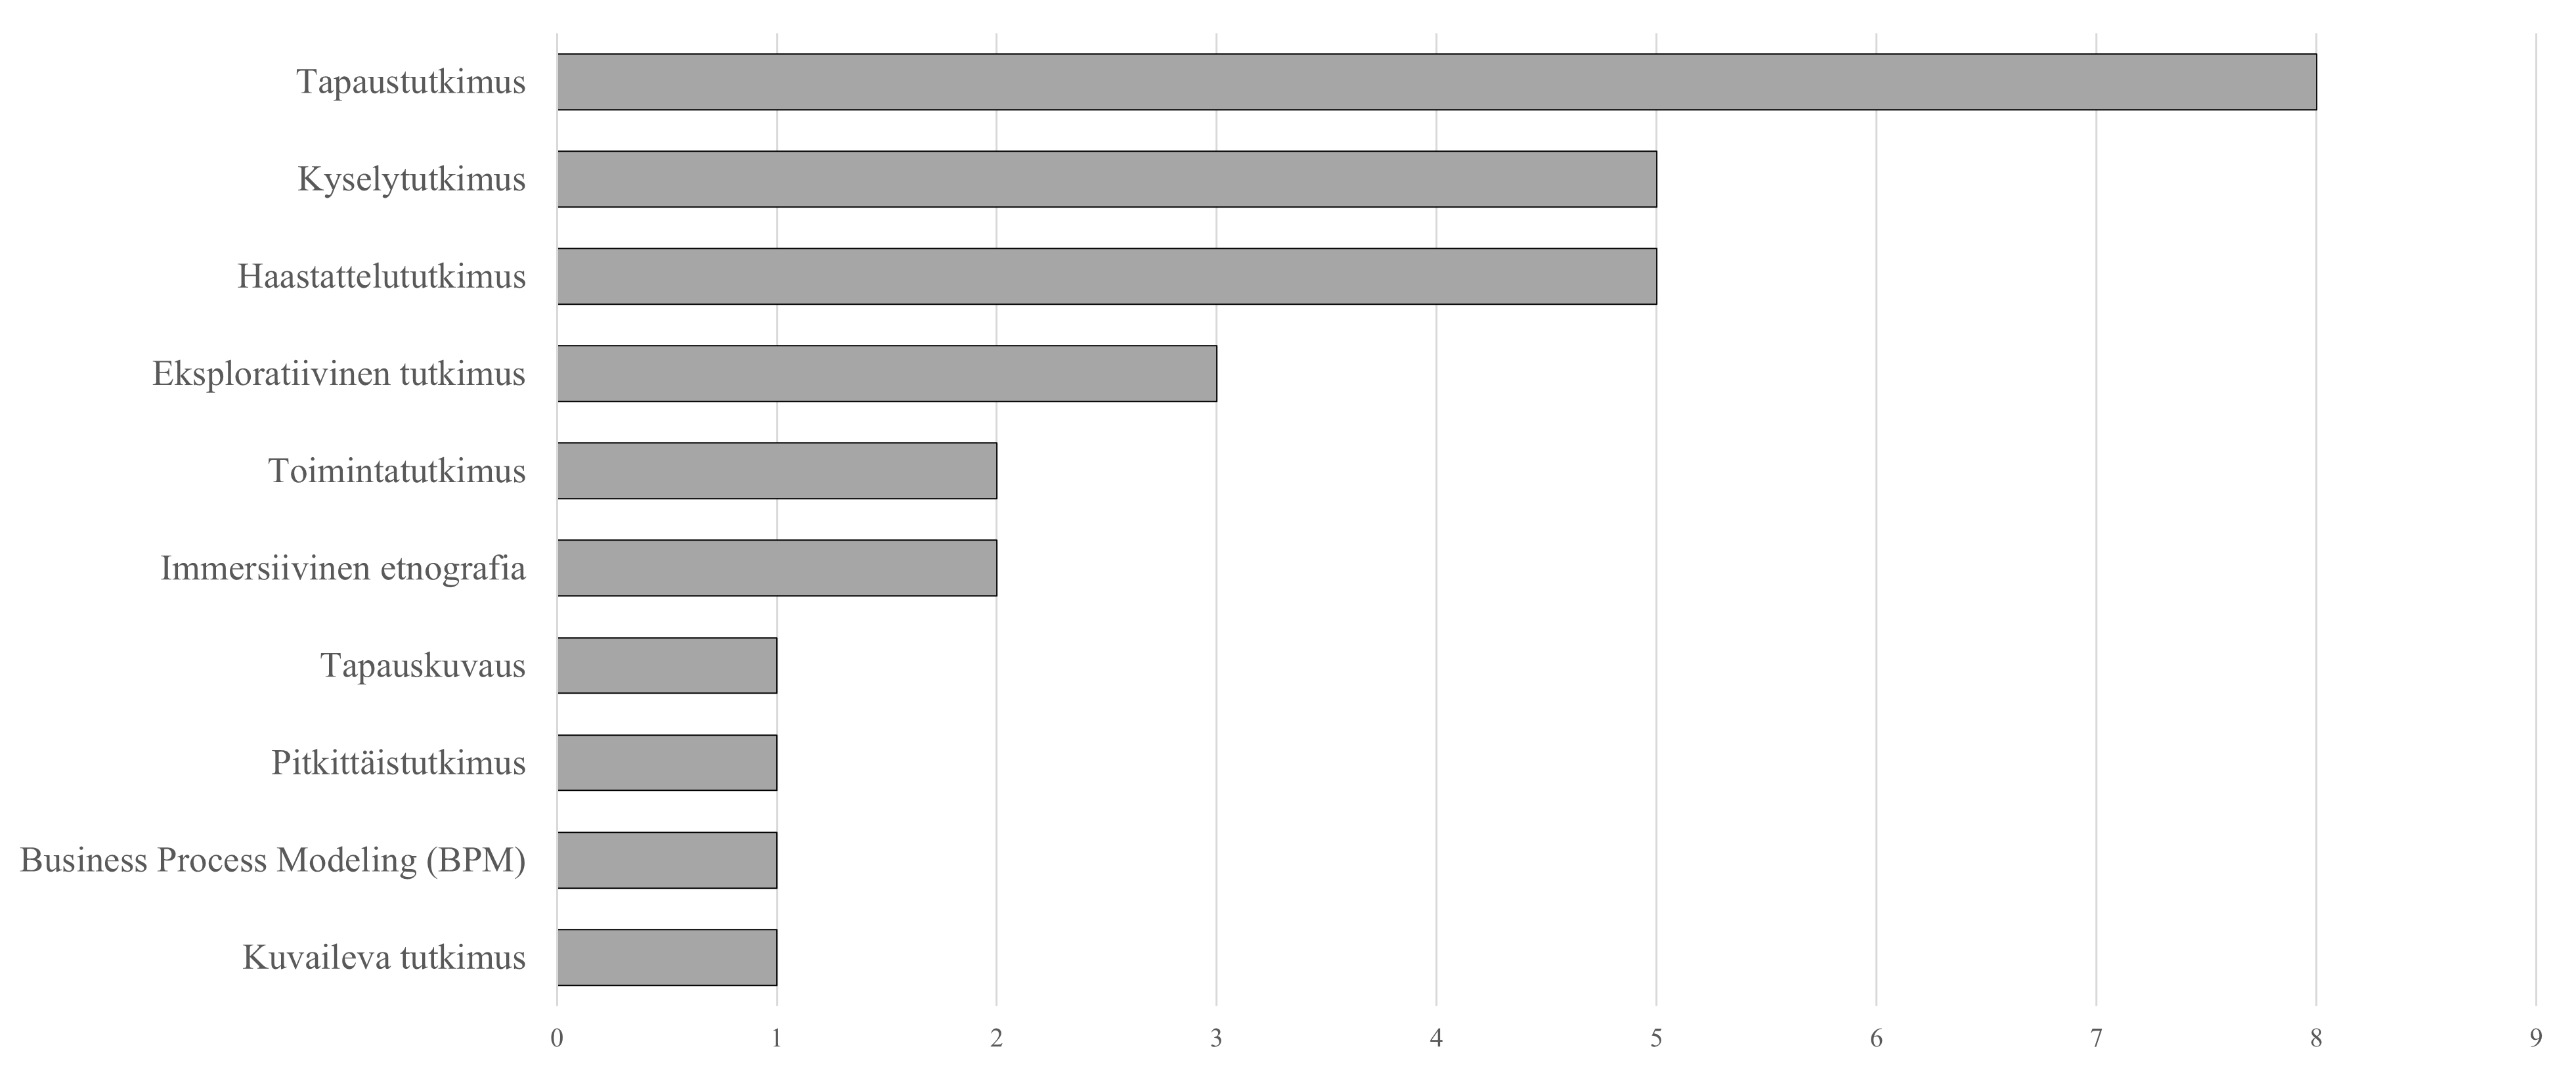
\includegraphics[width=\textwidth]{media/tutkimusasetelmat.png}
    \caption{Artikkelien tutkimusasetelmien luonnehdinnat}
    \label{kuvio:tutkimustyypit}
\end{figure}

Artikkeleista kerättiin myös tiedot käytetyistä tutkimusmenetelmistä, joita kertyi yhteensä 12 erilaista (kuvio \ref{kuvio:tutkimusmenetelmat}). Eniten käytetty oli puolistrukturoitu haastattelu, jota käytettiin yhdentoista artikkelin tutkimuksessa. Kyselyä taas käytettiin seitsemässä: esimerkiksi \textcite{kulkarni-ym-2010} toteuttivat kyselyt vastavalmistuneille ohjelmistokehittäjille ja ohjelmistoalan yritysten HR-asiantuntijoille saadakseen tietoja yritysten perehdytyskäytännöistä. Aineistossa havainnointi (5) ja osallistuva havainnointi (2) saivat myös mainintoja. Grounded theory -menetelmä mainittiin neljässä artikkelissa. Esimerkiksi \textcite{viana-ym-2014} tutkivat sitä, miten ohjelmistokehitykseen liittyvä tieto siirtyy kokeneilta osaajilta tulokkaille. 

\begin{figure}[h]
    \centering
    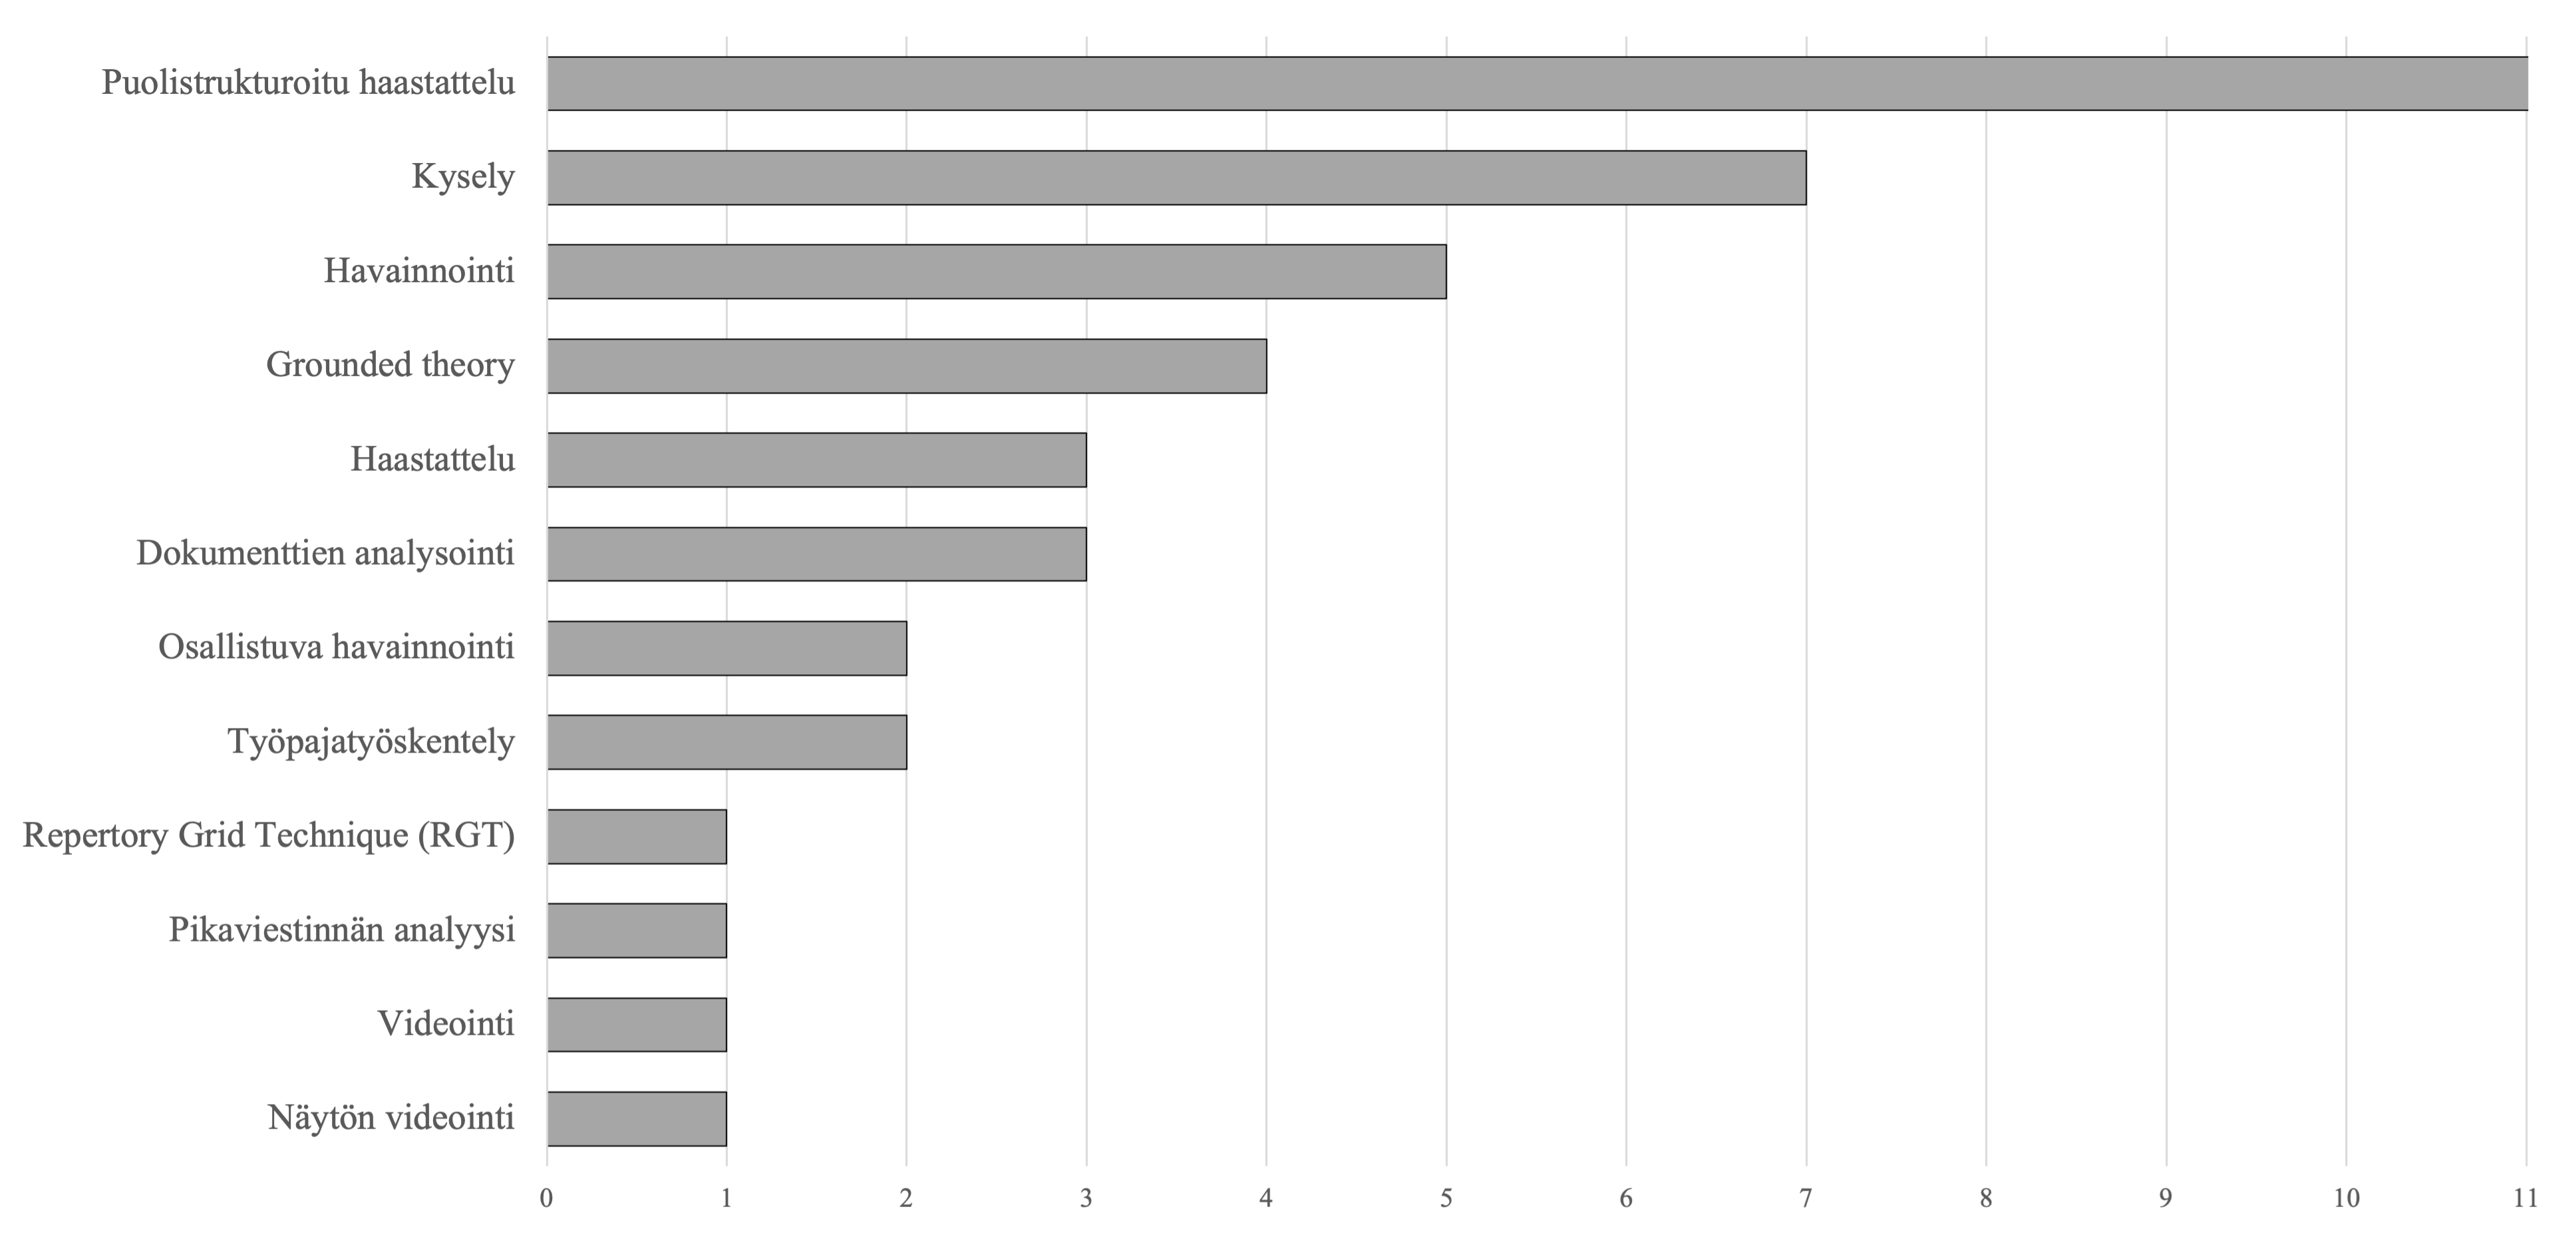
\includegraphics[width=\textwidth]{media/menetelmat.png}
    \caption{Artikkelien tutkimusmenetelmät}
    \label{kuvio:tutkimusmenetelmat}
\end{figure}

Tämän katsauksen tavoitteena oli selvittää, minkälaisia perehdytyskäytäntöjä ohjelmistoalan yrityksissä käytetään. Aineiston perusteella voidaan tehdä havaintoja siitä, miten primääritutkimusten tutkimusmenetelmien valinta vaikutti mainittujen perehdytyskäytäntöjen määrään. Kuviossa \ref{kuvio:menetelmilla-havaitut-kaytannot} on esitetty keskiarvot sille, montako perehdytyskäytäntöä keskimäärin mainittiin eri tutkimusmenetelmiä käyttäneissä artikkeleissa. Kuviosta voidaan havaita, että käytäntöjä löytyi eniten (15) tutkimuksissa joissa grid-menetelmä (engl. \textit{repertory grid technique}) oli mukana yhtenä tutkimusmenetelmänä.

Myös pikaviestinnän (ka. 8,0) ja dokumenttien (ka. 7,0) analysointi toi esiin useita käytäntöjä. Myös havainnointi tai osallistuva havainnointi (keskimäärin yht. 9,4) ja haastattelut (8,9) antoivat tietoa käytäntöjen määrästä. Videointi tai näytön videointi taas eivät olleet tehokkaita tapoja löytää käytäntöjä, sillä molemmilla löytyi keskimäärin yksi perehdytyskäytäntö.

\begin{figure}[h]
    \centering
    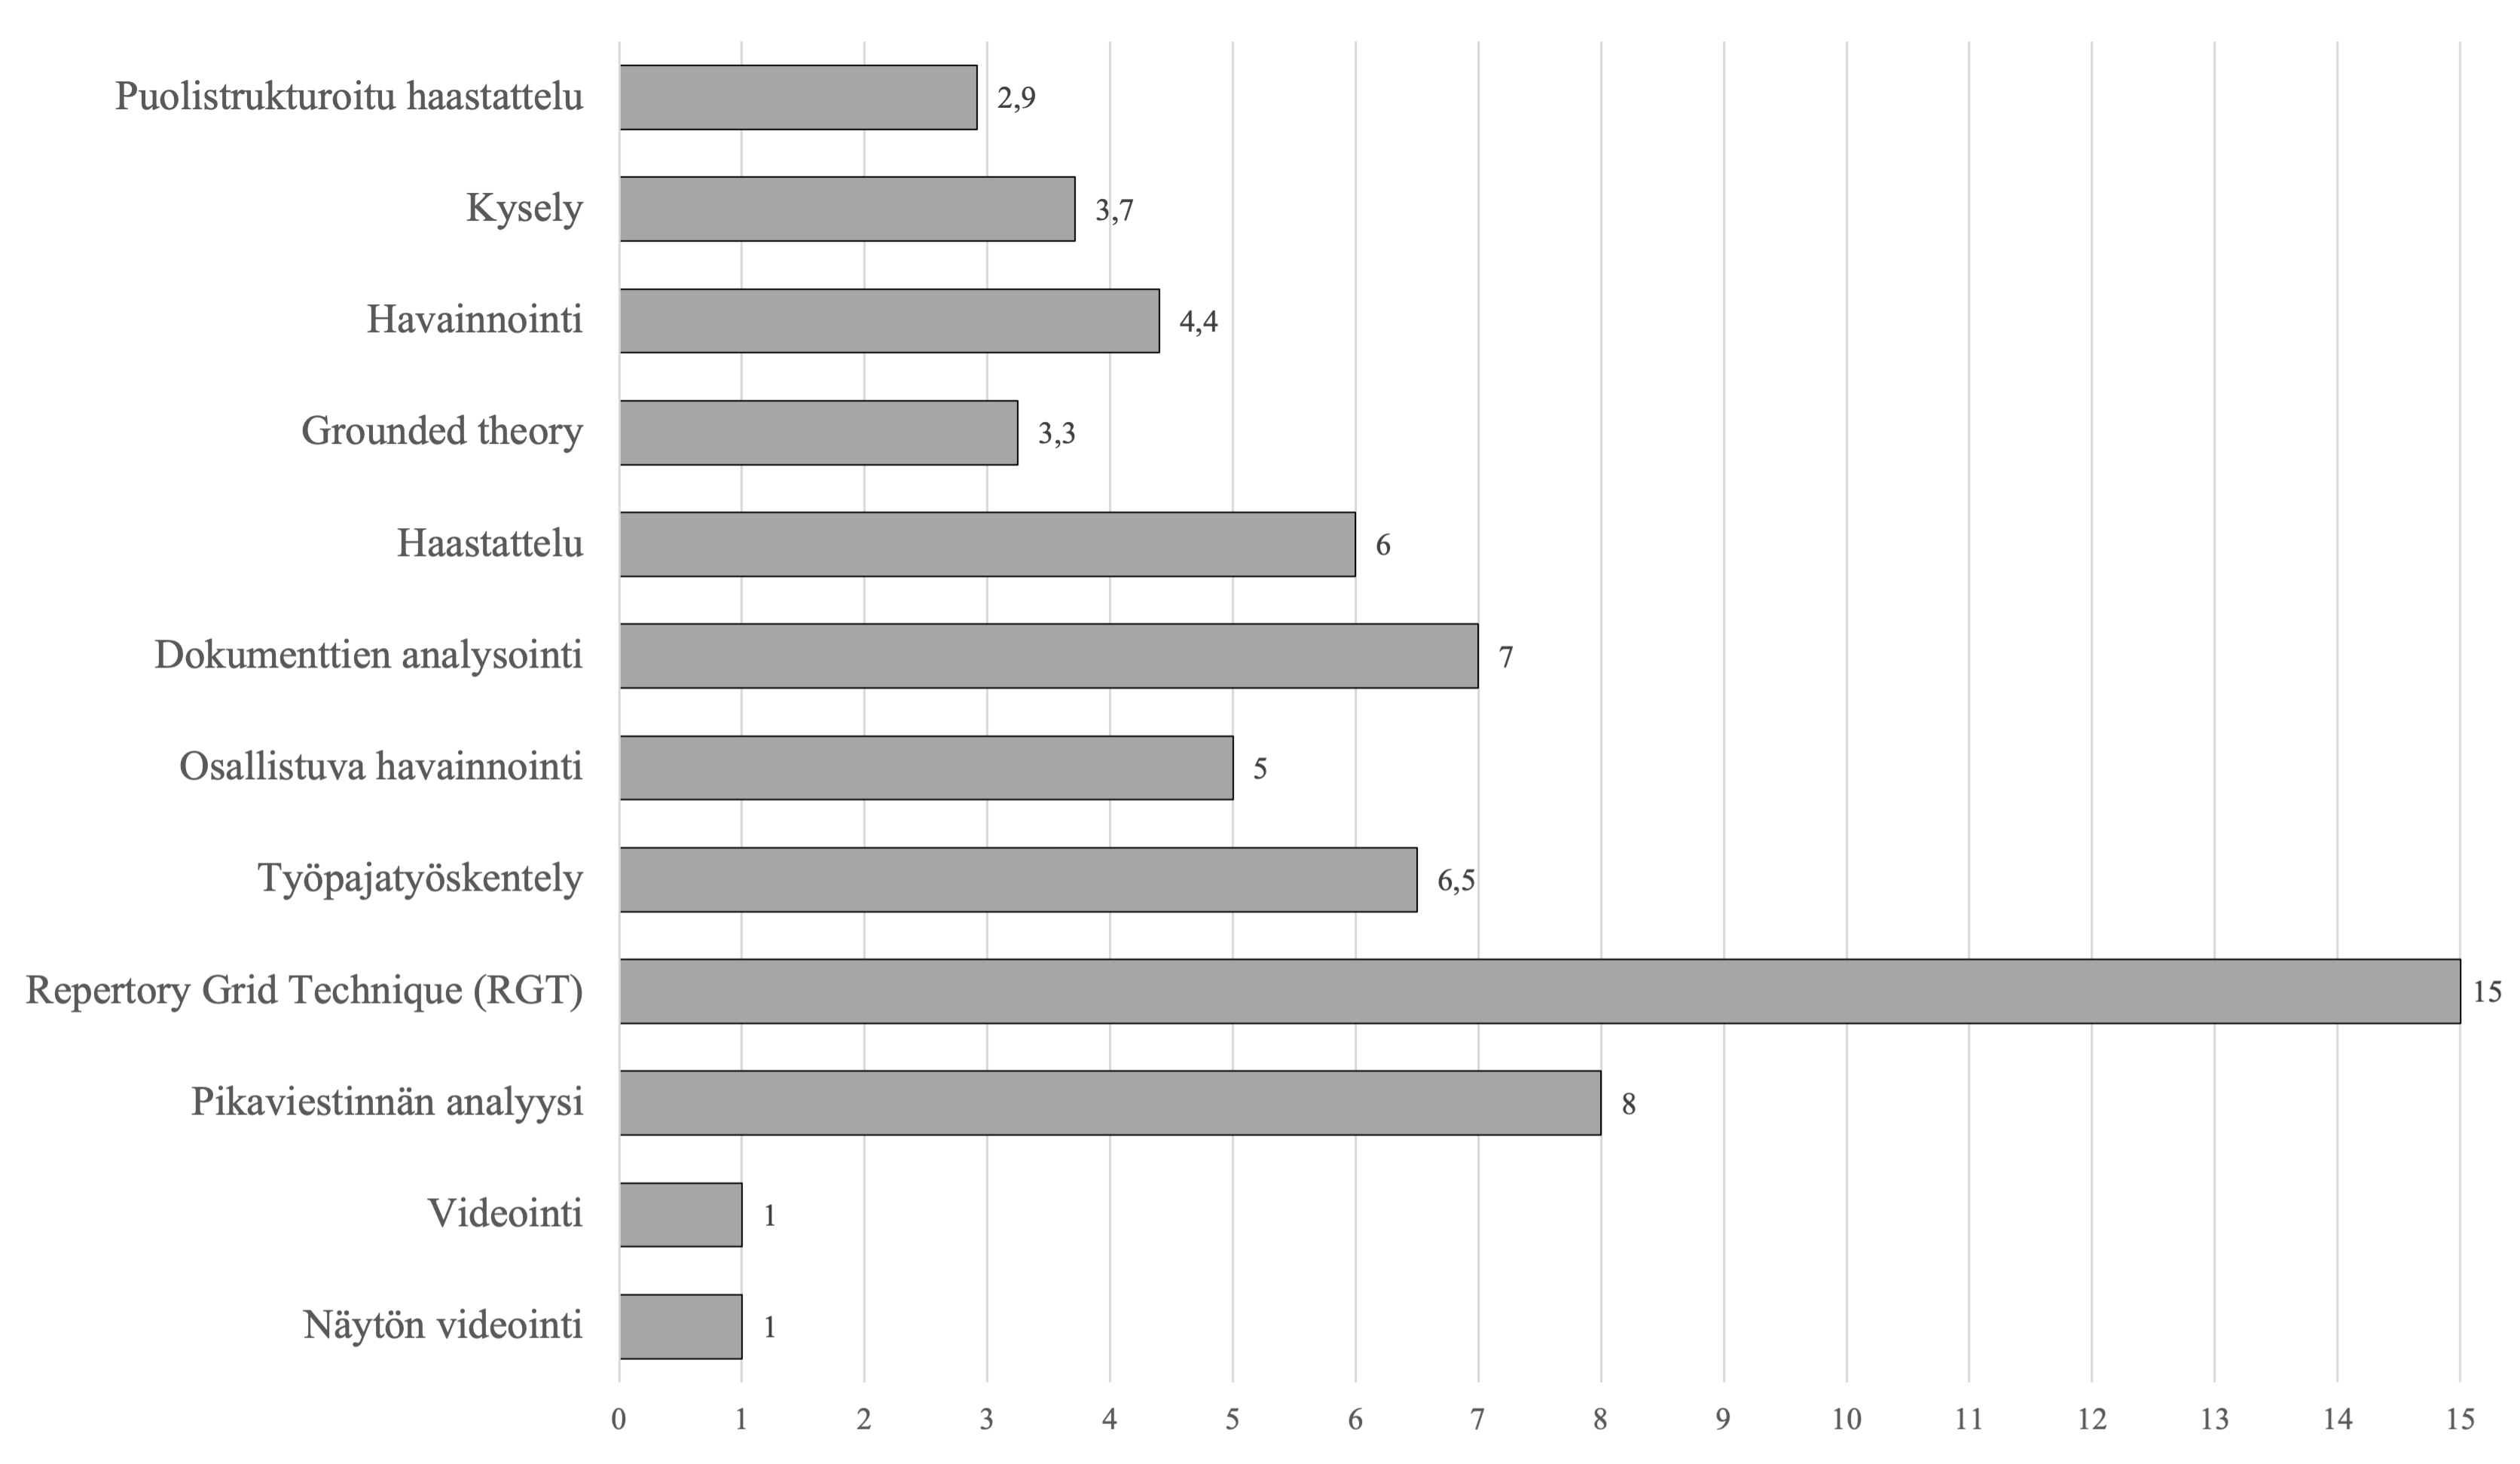
\includegraphics[width=\textwidth]{media/menetelmilla-havaitut-kaytannot.png}
    \caption{Keskiarvoiset artikkeleissa mainittujen perehdytyskäytäntöjen määrät tutkimusmenetelmittäin}
    \label{kuvio:menetelmilla-havaitut-kaytannot}
\end{figure}

\section{Tutkimuskohteiden kontekstit ja kohderyhmät}
\label{luku-tulokset-kontekstit-kohderyhmät}

Katsauksen tutkimusten yrityksissä tulokkaita perehdytettiin eri konteksteissa (ks. kuvio \ref{kuvio:kontekstit}). Eniten mainittu konteksti artikkeleissa oli \textit{Agile} eli ketterät menetelmät, joka mainittiin seitsemässä artikkelissa kahdestakymmenestä. Seuraavaksi eniten, viisi mainintaa, saivat globaalisti hajautettu ohjelmistokehitys ja suuret yritykset. Esimerkiksi \textcite{johnson-senges-2010} kertovat Googlen sekä \textcite{rodeghero-ym-2021} \textcite{ju-ym-2021} Microsoftin perehdytyskäytännöistä. Etätyöskentely, pienet yritykset, yrityksen järjestämä akatemia ja keskikokoiset yritykset olivat kontekstina kukin kahdessa artikkelissa. Esimerkiksi \textcite{rodeghero-ym-2021} raportoivat koronapandemian aikana työnsä aloittaneiden ohjelmistokehittäjien perehdyttämisestä.

\begin{figure}[h]
    \centering
    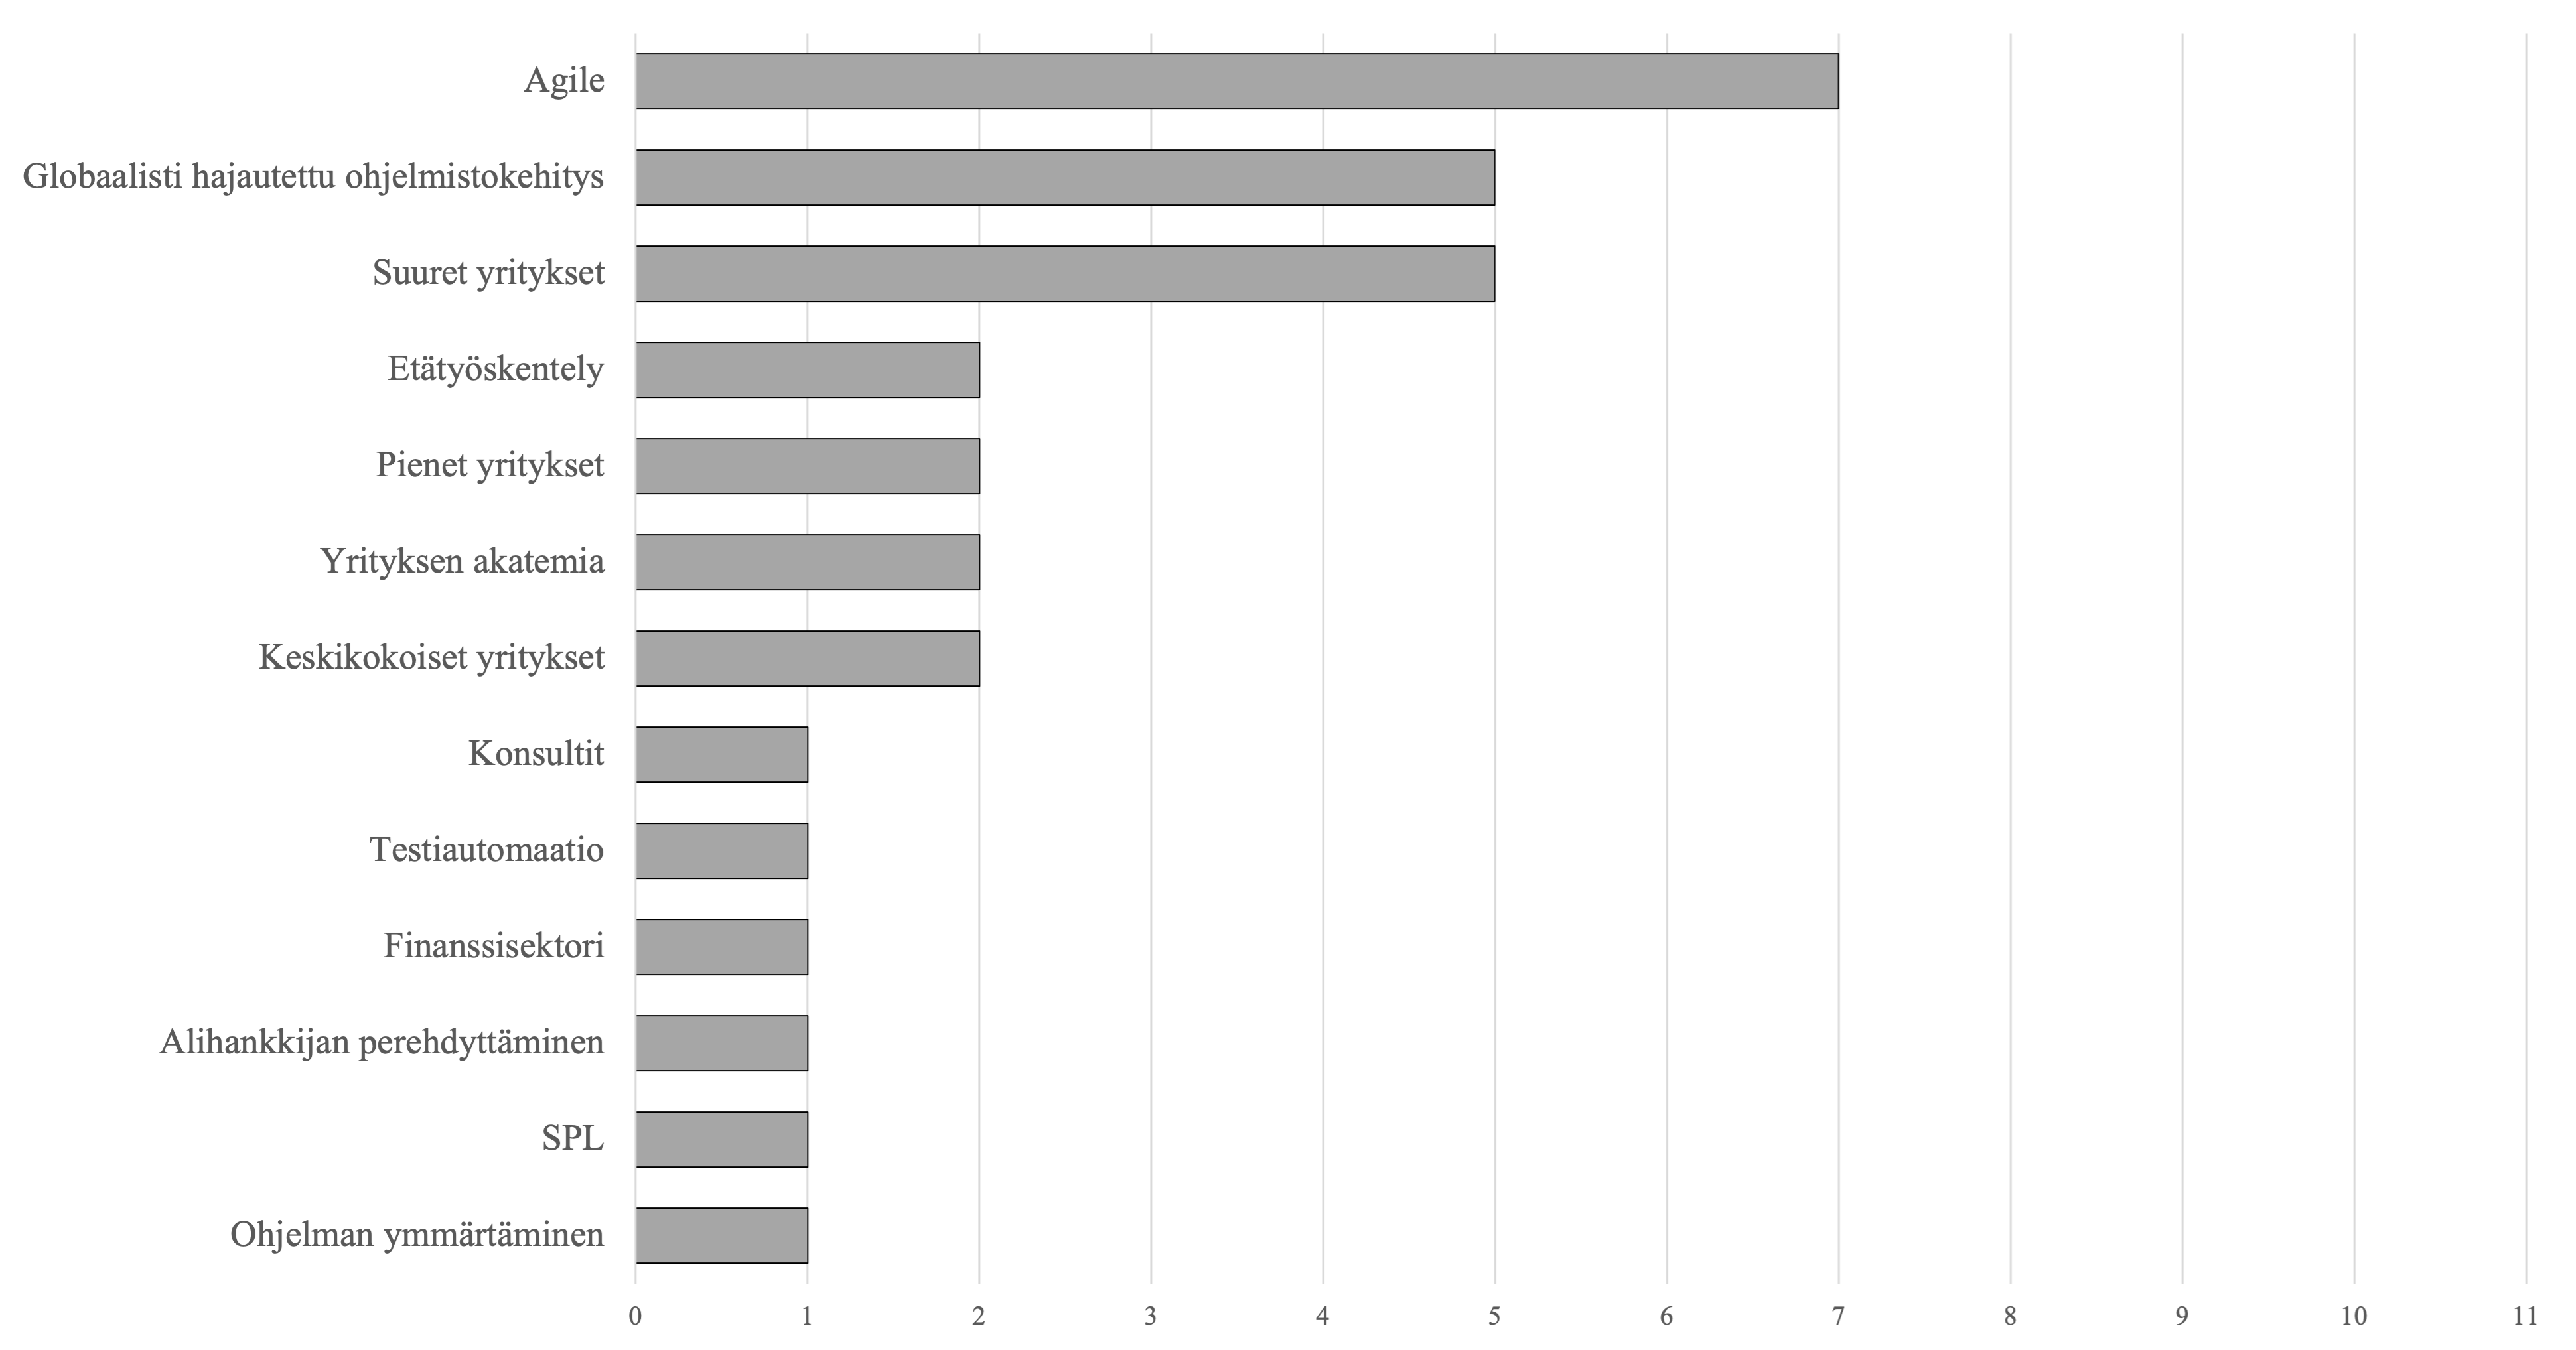
\includegraphics[width=\textwidth]{media/kontekstit.png}
    \caption{Artikkeleissa havaitut perehdytyksen kontekstit}
    \label{kuvio:kontekstit}
\end{figure}

Katsauksen artikkelien tutkimuksissa kohderyhmänä olivat useimmiten tulokkaat. Myös kokeneita, junior-ohjelmistokehittäjiä ja esihenkilöitä oli tutkittu, kuten kuviosta (\ref{kuvio:kohderyhmat}) ilmenee. Yhtä lukuun ottamatta kaikissa artikkeleissa kohderyhmänä oli ohjelmistokehittäjät yleisesti, olivat he sitten tulokkaita, vastavalmistuneita, junioreja tai kokeneita. Näiden lisäksi yhdessä artikkelissa kohderyhmänä olivat loppuvaiheen opiskelijat.

\begin{figure}[h]
    \centering
    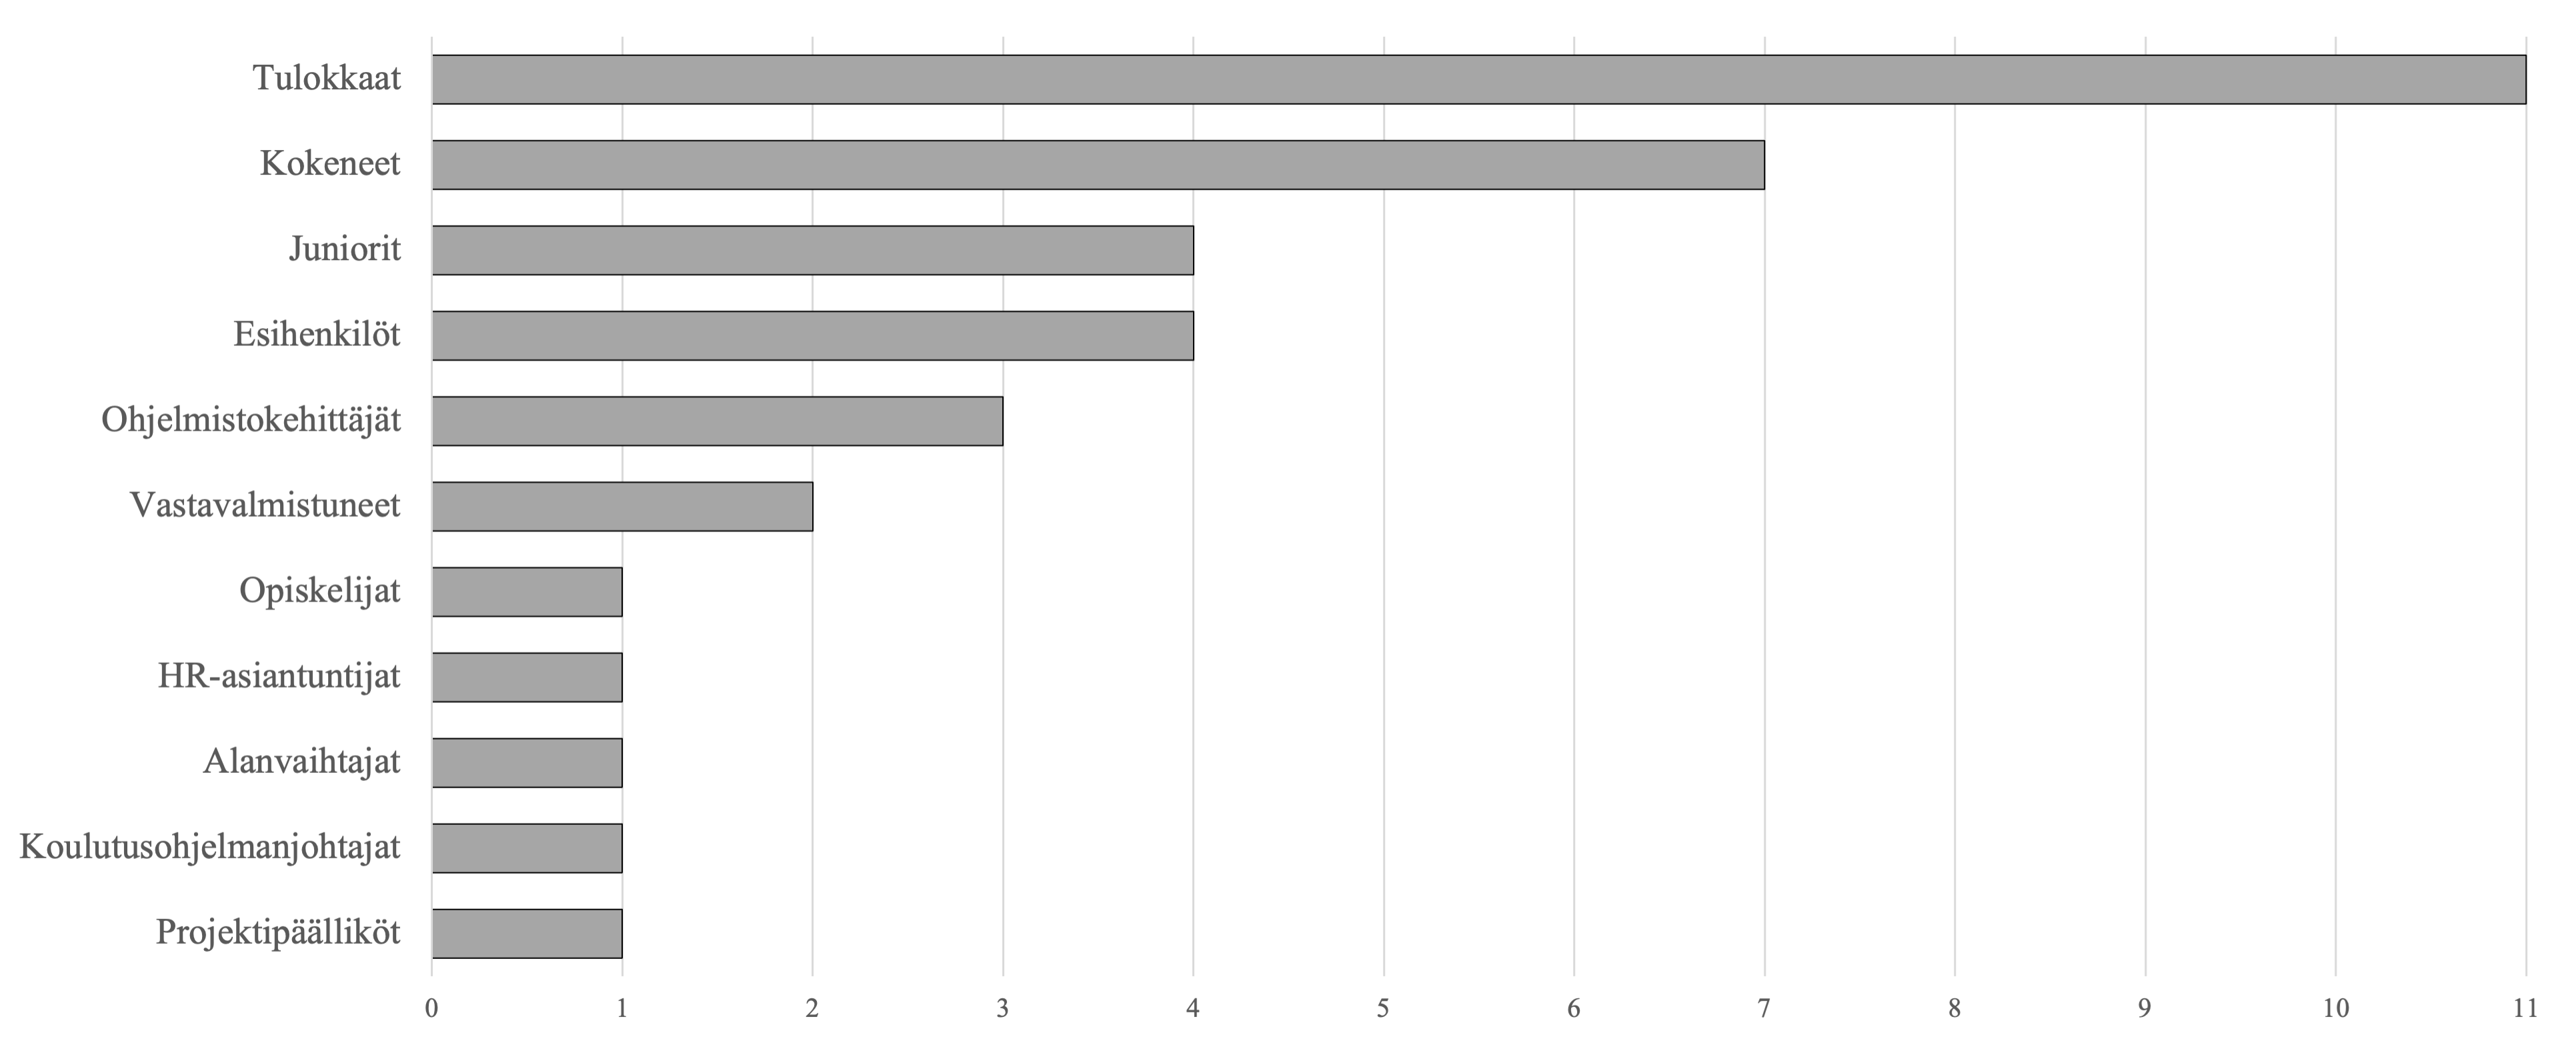
\includegraphics[width=\textwidth]{media/kohderyhmat.png}
    \caption{Artikkeleissa havaitut kohderyhmät}
    \label{kuvio:kohderyhmat}
\end{figure}

\newpage
\section{Artikkelien rakenteen arviointi}
\label{luku-artikkelien-rakenteen-arviointi}

Katsauksen artikkeleiden rakennetta arvioitiin käyttämällä kymmenosaista kriteeristöä, jossa arvioidaan sitä, missä määrin artikkelit sisältävät tiettyjä rakenteellisia elementtejä, joita American Psychological Association -järjestö pitää välttämättöminä ihmisiä tutkiville empiirisille tutkimuksille. Artikkeliin tulee sisältyä esimerksi tiivistelmä, kirjallisuuskatsaus ja tutkimuskysymysten määrittely (\textcite{apa-2001}, \textcite{randolph-ym-2008} mukaan). Tässä katsauksessa kriteeristöä täydennettiin vielä kahdella kriteerillä (\textit{Rajoitteita arvioitu} ja \textit{Tuloksia arvioitu suhteessa aiempaan tutkimukseen}). Taulukossa \ref{tbl:rakenteen-kriteerit} esitellään kukin kriteeri ja tiedot siitä, moniko artikkeli täytti kriteerin (lukumäärä ja prosentuaalinen osuus). Kaikissa artikkeleissa oli tiivistelmä eli abstrakti. Niinikään kaikissa artikkeleissa oli esitelty tutkimuksen tutkimusongelma. Tutkimusympäristöt ja -menettelyt sekä tutkimusten tavoitteet ja niissä käytetyt mittarit oli kuvattu valtaosassa artikkeleista. Rajoitteita arvioitiin 70 prosentissa artikkeleista. Tutkimuskysymys tai -kysymykset määriteltiin eksplisiittisesti vain yhdessätoista artikkelissa kahdestakymmenestä. Yhtä monessa artikkelissa oli arvioitu saatuja tuloksia suhteessa aiempaan tutkimukseen. Rakenteen arviointikriteerien täyttyminen on kuvattu taulukossa \ref{tbl:rakenteen-kriteerit}. Oikeassa reunassa olevasta sarakkeesta ilmenee yhteenlaskettu toteutuneiden kriteerien lukumäärä. Valtaosassa artikkeleista kahdestatoista kriteeristä toteutui lähes kaikki, mutta osassa artikkeleista niistä toteutui alle puolet.
 
\begin{table}[h]
    \scriptsize
    \begin{tabular}{llll}
        \toprule
        & \textbf{Arviointikriteeri} & \textbf{Artikkelien lukumäärä} & \textbf{Prosentuaalinen osuus} \\
        \toprule
        A & Tiivistelmä mukana & 20 & 100 \% \\
        B & Tutkimusongelma esitellään & 20 & 100 \% \\
        C & Kirjallisuuskatsaus esitellään & 18 & 90 \% \\
        D & Tutkimuksen tavoitteet tai perustelut esitellään & 18 & 90 \% \\
        E & Tutkimuskysymykset tai hypoteesit esitellään & 11 & 55 \% \\
        F & Osallistujat kuvataan asianmukaisesti & 16 & 80 \% \\
        G & Tutkimusympäristö kuvataan asianmukaisesti & 19 & 95 \% \\
        H & Mittaristo kuvataan asianmukaisesti & 18 & 90 \% \\
        I & Tutkimusmenettelyt kuvataan asianmukaisesti & 19 & 95 \% \\
        J & Tulokset ja pohdinta erotettu toisistaan & 15 & 75 \% \\
        K & Tuloksia arvioitu suhteessa aiempaan tutkimukseen & 11 & 55 \% \\
        L & Rajoitteita arvioitu & 14 & 70 \% \\
        \bottomrule
    \end{tabular}
    \caption{Artikkelien rakenteen arviointikriteerit ja niiden täyttävien artikkelien osuudet}
    \label{tbl:rakenteen-kriteerit}
\end{table}

\setlength{\LTcapwidth}{\textwidth}
\begin{scriptsize}
    \begin{longtable}[c]{| l | c | c | c | c | c | c | c | c | c | c | c | c | c | c | c | c |}
    
    \hline
    \multicolumn{1}{|c}{} & \multicolumn{16}{| c |}{\textbf{Artikkelien rakenteen arviointikriteeri (selite ks. kuvio \ref{tbl:rakenteen-kriteerit})}} \\
        \hline
            & \textbf{A} & \textbf{B} & \textbf{C} & \textbf{D} & \textbf{E} & \textbf{F} & \textbf{G} & \textbf{H} & \textbf{I} & \textbf{J} & \textbf{K} & \textbf{L} & \textbf{yht}  \\
        \hline
    \endfirsthead

    \hline
    \multicolumn{14}{|c|}{Taulukko jatkuu}\\
        \hline
            & \textbf{A} & \textbf{B} & \textbf{C} & \textbf{D} & \textbf{E} & \textbf{F} & \textbf{G} & \textbf{H} & \textbf{I} & \textbf{J} & \textbf{K} & \textbf{L} & \textbf{yht}  \\
        \hline
    \endhead
 \hline
 \endfoot

 \hline
 \caption{Artikkelien rakenteen arviointikriteerien täyttyminen}
 \endlastfoot


\textcite{rodeghero-ym-2021} & x & x & x & x & x & x & x & x & x & x & x & x & 12\\ \hline
\textcite{azanza-ym-2021} & x & x & x & x &   & x & x & x & x & x &   & x & 10\\ \hline
\textcite{ju-ym-2021} & x & x & x & x & x & x & x & x & x & x & x & x & 12\\ \hline
\textcite{britto-ym-2020} & x & x & x & x & x & x & x & x & x & x & x & x & 12\\ \hline
\textcite{yates-ym-2020} & x & x & x & x & x & x & x & x & x & x & x & x & 12\\ \hline
\textcite{moe-ym-2020} & x & x & x & x & x & x & x & x & x & x & x & x & 12\\ \hline
\textcite{kumar-wallace-2019} & x & x & x & x & x & x & x & x & x & x & x & x & 12\\ \hline
\textcite{viviani-murphy-2019} & x & x & x & x &   & x & x & x & x & x & x &   & 10\\ \hline
\textcite{buchan-ym-2019} & x & x & x & x & x & x & x & x & x & x &   & x & 11\\ \hline
\textcite{tuzun-ym-2018} & x & x & x & x &   & x & x & x & x & x &   & x & 10\\ \hline
\textcite{matturro-ym-2017} & x & x & x & x & x & x & x & x & x & x & x & x & 12\\ \hline
\textcite{britto-ym-2017} & x & x & x & x & x & x & x & x & x & x & x & x & 12\\ \hline
\textcite{pham-ym-2017} & x & x & x & x & x & x & x & x & x & x & x & x & 12\\ \hline
\textcite{kumar-ym-2016} & x & x & x &   &   &   & x &   & x &   &   &   & 5\\ \hline
\textcite{shannon-pool-2016} & x & x &   &   &   &   & x & x & x & x &   &   & 6\\ \hline
\textcite{viana-ym-2014} & x & x & x & x &   & x & x & x & x & x & x & x & 11\\ \hline
\textcite{hemphill-begel-2011} & x & x & x & x &   & x & x & x & x &   &   & x & 9\\ \hline
\textcite{kulkarni-ym-2010} & x & x &   & x & x & x & x & x & x &   &   &   & 8\\ \hline
\textcite{johnson-senges-2010} & x & x & x & x & x & x & x & x & x & x &   & x & 11\\ \hline
\textcite{bjornson-dingsøyr-2005} & x & x & x & x &   &   &   &   &   &   &   &   & 4\\
\hline
\hline
\textbf{Yhteensä kpl} & 20 & 20 & 18 & 18 & 11 & 16 & 19 & 18 & 19 & 15 & 11 & 14 & \\
\hline
\textbf{Prosentuaalinen osuus} & 100  & 100 & 90 & 90 & 55 & 80 & 95 & 90 & 95 & 75 & 55 & 70 & \\
 
\end{longtable}
\end{scriptsize}


\chapter{Pohdinta}
\label{paaluku-pohdinta}

TODO metateksti

\section{Perehdytyskäytännöt}

Katsauksen perehdytyskäytäntöihin liittyvien tulosten (luku \ref{luku-tulokset-kaytannot}) perusteella voidaan todeta, että mentorointi vaikuttaa olevan tärkeässä asemassa ohjelmistokehittäjien perehdyttämisessä. \textcite{viviani-murphy-2019} kuitenkin toteavat, että vahvasti mentorointiin nojaava perehdytyskäytäntö saattaa muodostua mentorille itselleen taakaksi. Myös \textcite{moe-ym-2020} toteavat, että mentoreiden saattaa olla haastavaa jakaa työaikaansa omien työtehtäviensä ja mentoroinnin välillä. \textcite{britto-ym-2017} täydentävät, että erityisesti pitkään käynnissä olleissa nk. legacy-projekteissa tulokkaat joutuvat turvautumaan mentorin apuun usein, mikä vaikuttaa mentorien tuottavuuteen ja työtyytyväisyyteen. Tässä katsauksessa tunnistettu tulokkaiden keskinäisen yhteistoiminnallisen oppimisen ulottuvuus voisi keventää mentorien työtaakkaa: mikäli organisaatiossa aloittaa samaan aikaan useita uusia työntekijöitä, voisi perehdyttämisprosessissa painottaa tulokkaiden keskinäistä yhteistoimintaa vertaisryhmänä. Yhteistyötä vaativat työtehtävät voisivat auttaa tulokkaita perehtymään organisaatiossa tehtävään työhön, kehitettäviin tuotteisiin ja olemassaolevaan ohjelmistokoodiin. Tulokkailla on myös paljon osaamista, jonka jakautumista vertaisryhmässä työskentely voisi edistää. Työskentelyssä ilmenevät pulmatilanteet tulokkaat voisivat pyrkiä ratkaisemaan ensin yhdessä ja konsultoimaan nimettyä mentoria vasta tarvittaessa. Tällaiset menetelmät toki edellyttävät, että sosialisaatioresurssien teorian yhdeksänteen ulottuvuuteen, työn tekemisen resursseihin, liittyvä valmistelu on tehty organisaatiossa huolellisesti. Esimerkiksi sisäisen teknisen dokumentaation tulisi olla ajantasaista ja riittävän tarkkaa.

Työtehtäviin ja työn luonteeseen liittyvät käytännöt ovat katsauksen tulosten mukaan myös oleellisia perehdyttämisessä. Työyhteisössä voidaan varautua uuden työntekijän aloitukseen esimerkiksi valmistelemalla hänelle etukäteen projekti tai valitsemalla tulokkaalle erityisen hyvin sopivia, suoraviivaisia työtehtäviä (nk. \textit{Good First Issue}). Kuten \textcite{ju-ym-2021} toteavat, työtehtävien haastavuuden tulisi kuitenkin pian nousta, jotta tulokas saa haastavia tehtäviä, mikä puolestaan pitää yllä motivaatiota.

Kuten \textcite{britto-ym-2020} toteavat, että perehdytysprosessit tulee suunnitella huolellisesti. Mielenkiintoinen jatkotutkimusaihe olisi se, miten perehdytysprosesseja strukturoimalla ja suunnittelemalla voitaisiin edistää organisatorisen sosialisaation toivottuja tuloksia kuten työntekijöiden tyytyväisyyttä, työhön sitoutumista ja työssä suoriutumista.

Erityisen mielenkiintoista on tarkastella niitä sosialisaatioresurssien teorian ulottuvuuksia, joihin liittyviä käytäntöjä katsauksessa ei löydetty yhtään. Näitähän olivat tulokkaan tunnustukseen tai arvostukseen (\#15), perehdytysprosessin seurantaan (\#16) ja sosiaalisiin suhteisiin (\#8) liittyvät ulottuvuudet. Sosiaalisiin suhteisiin liittyvien käytäntöjen puutetta katsauksessa voidaan selittää sillä, että sosialisaatioresurssien teoriassa sitä sivuaa kaksi muuta ulottuvuutta: sosiaaliset tapahtumat (\#5) ja sosialisaatioagentit (\#6), joihin liittyviä käytäntöjä kyllä havaittiin. Sosiaalisiin suhteisiin liittyvät käytännöt viittaavat \textcite{wanberg-2012} mukaan erilaisia toimia, jotka auttavat tulokkaita muodostamaan sosiaalisia suhteita: esimerkiksi esittäytymiset ja lyhyet keskustelut luetaan tähän ulottuvuuteen. Näitä käytäntöjä ei siis katsauksessa havaittu. Tätä saattaa selittää se, että esittäytyminen uudelle kollegalle ja tutustumiseen tähtäävät keskustelunavaukset kuuluvat pikemminkin yleisiin sosiaalisiin työyhteisötaitoihin kuin varsinaisiin perehdyttämiskäytäntöihin. 

\textcite{wanberg-2012} toteaa perehdytysprosessin seurannan tarkoittavan sitä, missä määrin organisaatio tarjoaa tulokkaille tukea muodollisen perehdyttämisjakson päätyttyä esimerkiksi varmistamalla työn sujumista tai tiedustelemalla avun tarpeita. Perehdytysprosessin seurantaan liittyviä käytäntöjä ei tässä katsauksessa havaittu lainkaan, mikä on mielenkiintoinen piirre aineistossa. Kun esihenkilön tukikin (ulottuvuus 7) mainittiin vain neljässä artikkelissa, olisi jatkotutkimuksissa perusteltua selvittää, miten uusien työntekijöiden työskentely sujuu perehdyttämisen jälkeen ja minkälaista tukea heille tarjotaan.

Tulokkaan arvostamisen ja tunnustuksen antamisen ulottuvuuteen liittyviä käytäntöjä ei myöskään löydetty lainkaan. \textcite{wanberg-2012} määrittelee tämän ulottuvuuden liittyvän siihen, missä määrin uudet tulokkaat saavat tunnustusta ja kiitosta ponnisteluistaan ja suorituksistaan, mikä on heidän mukaansa erityisen tärkeää työsuhteen alkuvaiheessa, jolloin työntekijä pyrkii jäsentämään uutta ympäristöään ja rooliaan siinä. Ulottuvuuteen liittyy läheisesti myös palautteen ulottuvuus (\#14), johon liittyviä käytäntöjä mainittiin yhdessätoista artikkelissa. Nämä ulottuvuudet ovat käsitteellisesti lähellä toisiaan, joten on mahdollista, että tulokkaan arvostamiseen ja tunnustukseen liittyviä käytäntöjä on katsauksessa tulkittu palautteena. Mahdollisia jatkotutkimusaiheita voisivat olla se, miten tulokkaiden saama arvostus ja palaute vaikuttavat perehtymisprosessin tuloksiin tai se, minkälaisia käytäntöjä ohjelmistokehityksen arkeen voidaan tuoda, jotta positiivinen ja palaute koituisi kaikkien työryhmän jäsenten osaksi. Voisiko esimerkiksi ketterien menetelmien kuten Scrumin säännöllisiä kokouksia rikastaa ääneen lausutulla arvostuksella ja kiitoksella?

Vain kahdessa artikkelissa mainittiin perehdytyskäytäntönä se, että tulokkaalle asetettaisiin tavoitteita, joiden saavuttamista arvioitaisiin. Mikä mahtaa selittää näin vähäistä määrää? Onko tavoitteiden asettaminen niin ilmiselvä käytäntö, ettei sitä artikkeleissa edes mainita, vai eikö tulokkaille todella aseteta tavoitteita? Lisätutkimusta tarvitaan asian selvittämiseksi.

\section{Näkökulmia perehdytyksen onnistumisen mittaamiseen}
\label{luku-näkökulmia-perehdytyksen-onnistustumisen-mittaamiseen}

Perehdytyksen onnistumista oli mitattu vain harvoissa artikkeleissa, joten tässä katsauksessa mittareista ei juuri saatu tietoa. \textcite{britto-ym-2020} mittasivat globaalisti hajautettujen ohjelmistokehitystiimien tuottavuutta ja autonomiaa. Heidän tutkimuksessaan Intiassa toimivat ohjelmistokehittäjät tekivät ison, monimutkaisen, paljolti nk. legacy-koodista koostuvan tietojärjestelmän räätälöintityötä. Jokaisen työtehtävän kompleksisuus ja koko arvioitiin, jotta pystyttiin mittaamaan tiimien suoriutumista numeerisesti. Arviointiin osallistuivat myös kokeneet sovellusarkkitehdit. \textcite{britto-ym-2020} kertovat tulosten mukaan tulokkaiden suorituskyvyn kasvavan hitaasti. Kahden vuoden jälkeen tulokkaat olivat edelleen keskimäärin 3,57 kertaa vähemmän tuottavia ja 1,67 kertaa vähemmän itsenäisiä kuin tavoitteeksi asetetut vertailuryhmät. \textcite{britto-ym-2020} toteavat, että suorituskyky lienee tavoitetasolla aikaisintaan kolmen vuoden kuluessa, mutta siihen voi kulua jopa viisi vuotta. Katsauksen ulkopuolisen kirjallisuuden perusteella \parencite{casalnuovo-ym-2015} voidaan todeta, että vahvat ohjelmistokehittäjien väliset sosiaaliset suhteet edistävät tulokkaiden tuottavuuden kasvamista. \textcite{britto-ym-2020} toteavatkin, että heidän tutkimansa yritykset olivat pyrkineet vahvistamaan sosiaalisia suhteita lisäämällä videoneuvotteluita ja kasvokkaisia tapaamisia. 

Toisessa katsauksen artikkelissa \textcite{moe-ym-2020} vertailivat sitä, missä määrin perehdytyksen eri osa-alueet eli rekrytointi, orientaatio, tukityökalut ja -prosessit, palautetyökalut, koulutus sekä valmennus ja tuki \parencite{bauer-2010} tulivat katetuiksi perehdytyksen aikana kahdessa eri ohjelmistokehitystiimissä. \textcite{moe-ym-2020} kertovat erojen olleen pieniä ja johtuneen lähinnä siitä, että mentorointi toteutui tiimeissä eri tavoilla, sillä toisessa tiimissä osa mentoreista joutui lopettamaan mentoroinnin kokonaan.

\textcite{shannon-pool-2016} taas kertovat, että yrityksen omassa akatemiassa aloittaneiden tulokkaiden työpanos oli myönteinen jo kuuden viikon jälkeen. Tässä tutkimuksessa oli käytetty kymmentä eri perehdytyskäytäntöä. Tulokkaat toimivat vertaisryhmänä ja heille järjestettiin yhteinen muodollinen koulutusjakso. Sosiaaliset tapahtumat auttoivat vahvistamaan sosiaalisia suhteita ja tulokkaat saivat tukea myös mentorilta. Akatemia kesti yhteensä kuusi kuukautta ja se sisälsi sekä luokkahuoneessa tapahtuvaa opetusta että käytännön harjoituksia. Tulokkaat liittyivät koulutusjaksonsa jälkeen ohjelmistokehitystiimeihin, joiden mitattu työteho kyllä heikentyi ensimmäisten aluksi aikana, mutta palasi sitten tiimin aiempaan tahtiin. Tulokkaat tuottivat tiimiensä työskentelylle lisäarvoa jo varhaisessa vaiheessa, mutta erityisesti neljän kuukauden jälkeen. \parencite{shannon-pool-2016}.

Katsauksen ulkopuolelta voidaan todeta, että organisatorisen sosialisaation onnistumista on pyritty mittaamaan eri tavoin. \textcite{zhao-ym-2007-mittari} esittelevät Organizational Socialization Content Questionnaire -kyselyn, jonka avulla voidaan arvioida tulokkaan sosialisaation onnistumista organisaatiokulttuurin omaksumisen, työtehtävien osaamisen, ihmissuhteiden muodostumisen ja organisaatiopolitiikan ymmärryksen näkökulmista. \textcite{haueter-ym-2003} taas esittelevät Newcomer Socialization Questionnaire (NSQ) -mittarin, joka Likert -kyselyllä mittaa organisatorisen sosialisaation onnistumista kolmella osa-alueella: suhteessa organisaatioon, suhteessa tulokkaan työryhmään ja suhteessa tulokkaan työtehtäviin. Kuten luvussa \ref{luku-organisatorinen-sosialisaatio-ja-perehdyttäminen} mainittiin, organisatorisen sosialisaation liittyviä ilmiöitä on kirjallisuudessa kuvattu myös organisatorisen \textit{sopeutumisen} käsitteellä, jonka mittaamiseen \textcite{gailliard-ym-2010} esittelevät Organizational Assimilation Index -mittarin. Sen avulla voidaan määritellä sopeutumisen tekijöitä (työtehtävien osaaminen, tuttuus työtovereiden kanssa, tuttuus esihenkilöiden kanssa, osallistuminen, työkulttuuriin sopeutuminen, osallistuminen ja omaan työrooliin liittyvä neuvotteleminen) selvittämällä vastaajien samanmielisyyttä 24 väittämän suhteen (mm. ``Arvioin olevani asiantuntija työssäni” ja “Mielestäni esihenkilöni arvostaa mielipiteitäni'') \parencite{gailliard-ym-2010}. Mittarin Cronbachin alfa -luotettavuuskertoimet ovat vaihdelleet välillä .63--.95 \parencite{gailliard-ym-2010}. Mittaria on käytetty sosialisaatioresurssien teoriaa soveltavassa tutkimuksessa \parencite{cranmer-ym-2016}, jossa tutkittiin tulokkaiden saaman emotionaalisen, tiedollisen ja välineellisen tuen vaikutusta myöhempään työtyytyväisyyteen. \textcite{harris-ym-2022} taas esittelevät kehittämänsä mittarin, joka perustuu myös sosialisaatioresurssien teoriaan ja mittaa tulokkaiden saamia sosiaalisen pääoman resursseja, eli vain osaa teorian seitsemästätoista ulottuvuudesta. Esimerkkejä väittämistä ovat ``Kollegani antavat usein hyödyllistä apua'' (sosialisaatioagenttien ulottuvuus) ja  ``Uutena työntekijänä järjestettiin sosiaalinen tapahtuma, jossa minut toivotettiin tervetulleeksi (esim. tiimikahvit)'' (sosiaalisten tapahtumien ulottuvuus) \parencite{harris-ym-2022}.  

Nämä mittarit ovat kuitenkin yleiskäyttöisiä, joten ne eivät ota huomioon ohjelmistokehityksen alakohtaisia erityispiirteitä (ks. luvut \ref{luku-perehdyttämisen-erityisyys-ohjelmistoalalla} ja \ref{luku-tulokkaiden-haasteet}). Ohjelmistokehityksen alalla organisatorisen sosialisaation onnistumista mittaava tutkimus on niukkaa ja jäsentymätöntä. Aihetta on tutkittu lähinnä tuottavuuden näkökulmasta mittaamalla esimerkiksi commit-määriä eli tulokkaan tekemiä ohjelmistokoodin muutoksia tai aikaa työsuhteen alkamisesta ensimmäiseen tuotantoon vietyihin muutoksiin \parencites%
    {rastogi-ym-2017}%
    {fagerholm-ym-2013}%
\relax.
% 
Kun ohjelmistokehityksen tiedetään olevan haastavaa työtä erityisesti tulokkaille (ks. luku \ref{luku-tulokkaiden-haasteet}), olisi jatkotutkimusta tärkeä kohdistaa tulokkaiden sosialisaatioprosessin onnistumisen mittaamiseen tai jo kehitettyjen mittarien laajentamiseen.



\section{Tutkimusasetelmat ja -menetelmät}

Katsauksen tulosten perusteella voidaan todeta, että grid-menetelmän (engl. \textit{Repertory Grid Technique}, RGT) avulla havaittiin tehokkaasti käytettyjä perehdytyskäytäntöjä. \textcite{buchan-ym-2019} tutkivat tätä menetelmää käyttämällä sitä, mitkä perehdytyskäytännöt ovat tärkeitä eri perehdytystavoitteiden saavuttamisessa. Tutkimukseen osallistujilta saatiin tietoa kunkin tavoitteen saavuttamiseen hyödynnettävistä käytännöistä sekä näiden välisten yhteyksien vahvuudesta eli siitä, missä määrin käytäntö edistää tavoitteen saavuttamista. Tulosten mukaan esimerkiksi pariohjelmoinnin katsottiin edistävän tuotteen ja kohdealueen tuntemusta. Olemassaolevaan koodiin tutustumisen taas arvioitiin helpottavan ohjelmointi- ja testiautomaatiokäytäntöjen omaksumista. \parencite{buchan-ym-2019}.

\textcite{buchan-ym-2019} toteavat, että RGT:n pääkomponentit ovat (1) tutkimusaihe; (2) elementit, jotka ovat tutkimusaiheen ilmentymiä; (3) konstruktiot, jotka ovat ajatuksia, joita osallistujilla on elementeistä ja (4) yhteydet, jotka ovat elementtien ja konstruktioiden välisiä havaittuja suhteita. He ovat  käyttäneet menetelmää niin, että tutkimusaiheena oli ohjelmistokehittäjän perehdyttäminen. Elementteinä olivat perehdyttämisprosessin tavoitteet ja konstrukteina perehdytyskäytännöt. Linkkejä olivat näiden väliset yhteydet. Perehdyttämisprosessin tavoitteet oli määritelty tutkijoiden toimesta etukäteen. Perehdytyskäytännöt selvitettiin tutkimuskohteilta. Tämän menetelmän avulla saatiin siis paitsi tietoa perehdytyskäytännöistä, myös ammattilaisten käsityksiä niiden vaikuttavuudesta. 

RTG-menetelmää voisi hyödyntää niin, että tutkittaisiin tässä kirjallisuuskatsauksessa havaittujen 45 käytännön yhteyksiä perehtymisprosessin tavoitteisiin. Tässä katsauksessa eri käytäntöjen vaikuttavuutta ei arvioitu, joten jatkotutkimusta voitaisiin suunnata siihen. Vaihtoehtoisesti RGT-menetelmän elementteinä voisi olla SWEBOK (Software Engineering Body of Knowledge) -julkaisussa \parencite{swebok} kuvatut ohjelmistokehityksen yleiset osaamisvaatimukset. Tämä voisi auttaa räätälöimään perehdytysprosesseja yksilöllisempään suuntaan riippuen tulokkaan tuen tarpeista ja oppimistavoitteista -- onhan kullakin tulokkaalla omat vahvuutensa ja kehittämiskohteensa näiden osaamisvaatimusten alueilla. Perehdytysprosessin yksilöllistämistä suosittelevat myös \textcite{britto-ym-2017} ja \textcite{rodeghero-ym-2021}.

\section{Tutkimuskohteiden kontekstit ja kohderyhmät}

Mitä katsauksen tutkimuskohteiden perehdyttämiskonteksteista voidaan sitten päätellä? Ketterät menetelmät, globaalisti hajautettu ohjelmistokehitys tai etätyöskentely oli siis mainittu monissa, yhteensä kahdessatoista artikkelissa. Nämä ovat toki yleisiä ohjelmistokehityksen suuntauksia, mutta näissä konteksteissa myös hyvä perehdytys on erityisen tärkeää. \textcite{gregory-ym-2020} mukaan ketterän kehityksen konteksti aiheuttaa perehtymiselle haasteita, kun tulokkaan on omaksuttava myös ketterät toimintatavat ja ajattelutavat. 

\textcite{britto-ym-2017} toteavat, että etäällä toisistaan työskentelevien ohjelmistokehittäjien perehdyttäminen olisi yritysten haasteista peräti suurin erityisesti silloin, jos yrityksessä käytetään ketteriä menetelmiä. \textcite{britto-ym-2017} havaitsivat, että ketterät työskentelytavat merkitsivät sitä, että yrityksissä korostetaan enemmän verkostoitumista kollegoiden kanssa kuin edistymisen, työn tulosten ja työskentelytapojen dokumentointia. Juuri kattava ja ajantasainen dokumentaatio olisi kuitenkin tärkeä perehtymisresurssi erityisesti etänä työskenteleville tulokkaille. \textcite{moe-ym-2020} taas mainitsevat, että ketterien menetelmien käyttämisestä koitui tarve jatkuvalle työryhmän sisäiselle kommunikoinnille ja yhteistoiminnalle. Globaalisti hajautetuissa työryhmissä sekä maantieteellinen etäisyys että käytännön seikat, kuten aikaero, aiheuttavat haasteita tälle.

Katsauksen tutkimuksissa kohderyhmänä oli kuudessa artikkelissa junior-ohjelmistokehittäjät tai vastavalmistuneet. Kun tiedetään, että uudet ohjelmistokehittäjät kohtaavat ensimmäisissä työpaikoissaan monia haasteita (ks. luku \ref{luku-tulokkaiden-haasteet}, on hyvä että katsauksessa informantteina oli myös näitä työntekijöitä. Kuviossa \ref{kuvio:ulottuvuudet_kohderyhmat_juniorit} on esitelty sosialisaatioresurssien teorian ulottuvuudet, joihin liittyviä käytäntöjä näissä kuudessa artikkelissa havaittiin. Vertailun vuoksi kuviossa \ref{kuvio:ulottuvuudet_kohderyhmat_kokeneet_tai_hallinto} on vastaavat tiedot artikkeleissa, joissa kohderyhminä olivat esihenkilöt, projektipäälliköt, koulutusohjelmien johtajat, HR-asiantuntijat tai kokeneet ohjelmistokehittäjät. Oleellisin ero näissä osajoukoissa on se, että työn suunnittelun ulottuvuuteen liittyviä käytäntöjä ei mainittu lainkaan niissä artikkeleissa, joissa kohderyhminä oli juniorit tai vastavalmistuneet. Työn tekemisen resurssien ulottuvuuden käytäntöjä mainittiin vain yhdessä artikkelissa. Molemmat ulottuvuudet saivat viisi mainintaa muilta kohderyhmiltä. Olisinkin hyvä tutkia tarkemmin, miten junior-ohjelmistokehittäjien työskentelyä suunnitellaan joko perehdyttävän organisaation tai kehittäjien itsensä toimesta. Myös työn tekemisen resurssien ulottuvuuteen liittyviä käytäntöjä olisi syytä selvittää. Tämän katsauksen artikkeleista \textcite{yates-ym-2020} olivat valinneet näkökulmakseen ``information-push'':in, eli heitä kiinnosti se, miten organisaation aloitteesta tulokkaille siirretään tietoa. Työn tekemisen resurssien näkökulmasta voisi tutkia sitä, minkälaisin aloittein tulokkaat hyödyntävät esimerkiksi organisaation sisäistä dokumentaatiota tai olemassaolevaa koodia suoriutuakseen työtehtävistään. \textcite{gruman-ym-2006} tekemä tutkimus yliopisto-opiskelijoiden työharjoittelussa ilmenneiden perehdytyskäytäntöjen, tulokkaiden minäpystyvyyden, oma-aloitteisuuden ja sosialisaatiotulosten välisistä suhteista esittelee vahvan viitekehyksen, jonka kautta aihetta voisi tutkia myös sovelluskehityksen alalla.

\begin{figure}[h]
    \centering
    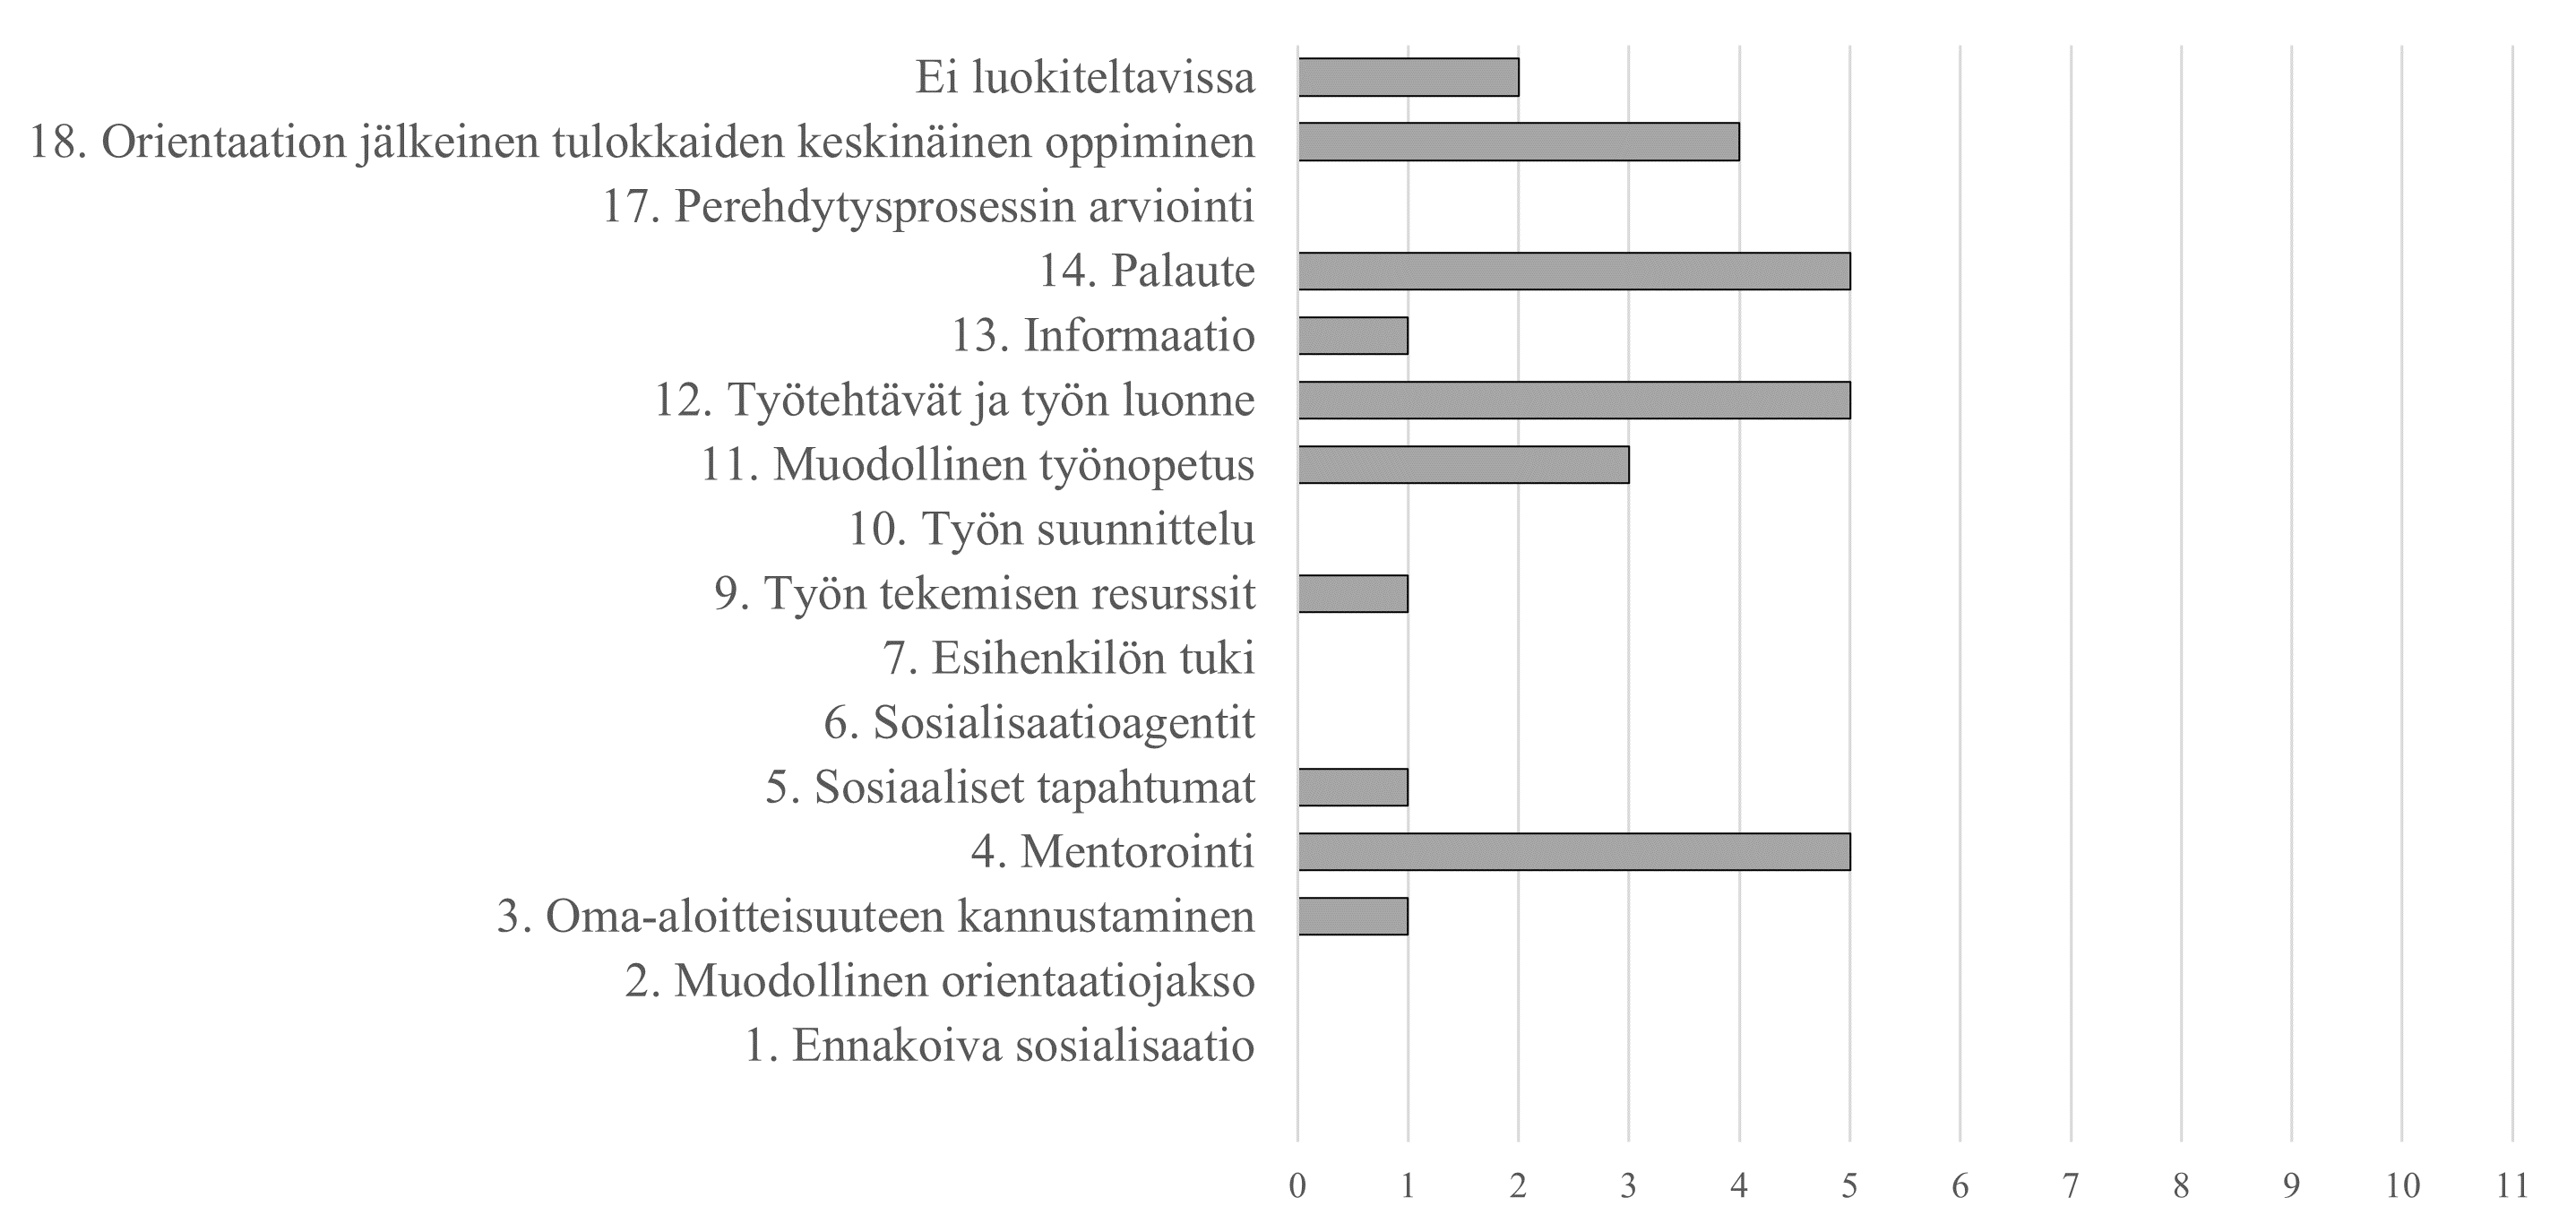
\includegraphics[width=\textwidth]{media/ulottuvuudet_kohderyhmat_juniorit-tai_vastavalmistuneet.png}
    \caption{Artikkeleissa havaitut sosialisaatioresurssien ulottuvuudet, kun kohderyhmänä juniorit tai vastavalmistuneet}
    \label{kuvio:ulottuvuudet_kohderyhmat_juniorit}
\end{figure}

\begin{figure}[h]
    \centering
    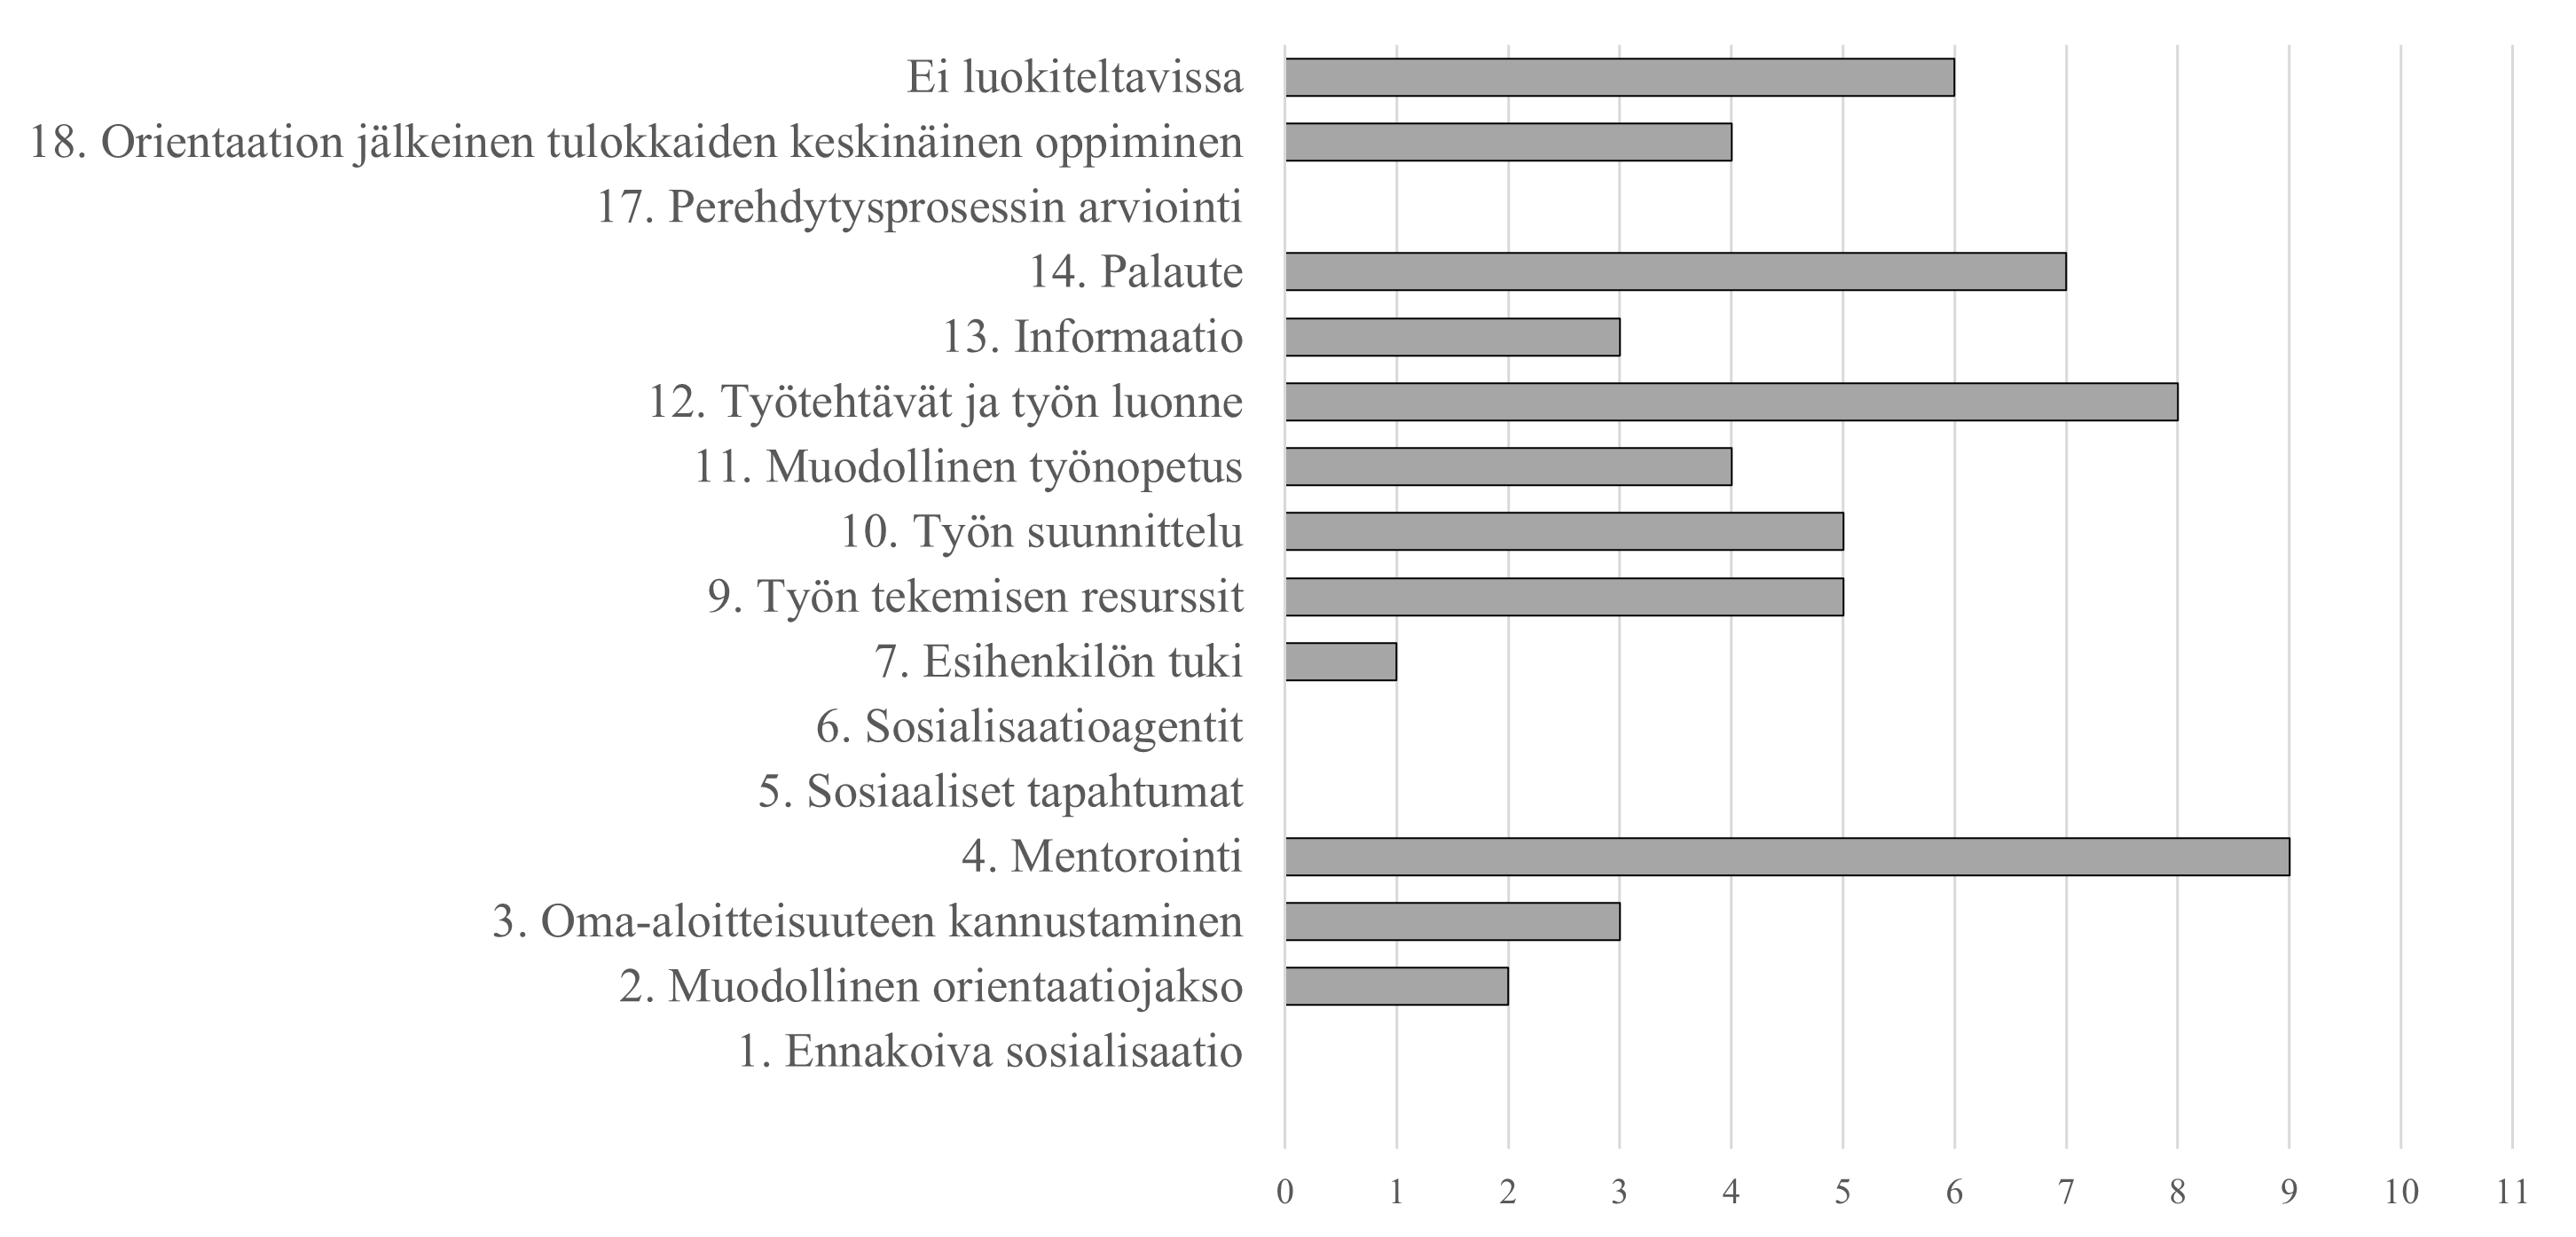
\includegraphics[width=\textwidth]{media/ulottuvuudet_kohderyhmat_kokeneet_tai_hallinto.png}
    \caption{Artikkeleissa havaitut sosialisaatioresurssien ulottuvuudet, kun kohderyhmänä kokeneet ohjelmistokehittäjät tai hallinnon työntekijät}
    \label{kuvio:ulottuvuudet_kohderyhmat_kokeneet_tai_hallinto}
\end{figure}

Tämän katsauksen artikkeleissa raportoitiin tutkimuksista erikokoisissa organisaatioissa. \textcite{viana-ym-2014} tutkivat 10 henkilön yritystä, \textcite{johnson-senges-2010} Googlen käytäntöjä ja \textcite{britto-ym-2020} Ericsson AB:ta. Laaja skaala erikokoisia organisaatioita vahvistaa katsauksen tulosten uskottavuutta.

Yksi katsauksen kiinnostavista löydöksistä oli yhdessä artikkelissa \parencite{kulkarni-ym-2010} mainittu työyhteisötaitokoulutus (engl. \textit{behavioral training}), jota järjestettiin lähes 80\%:ssa tutkituista yrityksistä. Tutkimuksen kyselyyn oli vastannut 32 intialaista IT-alan yritystä, joista kolmannes oli suuria (yli 10 000 työntekijää). Muodollisessa koulutuksessa vastavalmistuneille ohjelmistokehittäjille opetettiin tiimityöskentelyä, suullista ja kirjallista viestintää, johtamistaitoja sekä yritysmaailmassa ja asiakkaiden kanssa käyttäytymisen taitoja. Koulutus kesti keskimäärin 6--7 päivää. \parencite{kulkarni-ym-2010}. Tällaisen koulutuksen järjestäminen näyttää olevan siis tutkituissa yrityksissä varsin yleinen käytäntö. \textcite{kulkarni-ym-2010} toteavat, että Intiassa tapahtuu suuri osa globaalisti ulkoistetusta offshore-ohjelmistokehityksestä. \textcite{olson-olson-2003} kertovat kulttuuristen tekijöiden vaikuttavan globaalisti hajautetun ohjelmistokehityksen vuorovaikutukseen ja arkeen merkittävästi. Katsauksen löydös herättää pohdintoja siitä, onko tarpeen tutkia tarkemmin sitä, minkälaista perehdytyksen tulisi olla monikulttuurisissa tiimeissä, jotta kaikki tiimin jäsenet ymmärtävät toistensa odotukset, toimintatavat ja kulttuuriset seikat.

\section{Artikkelien rakenteen arviointi}
\label{luku-pohdinta-artikkelien-rakenteen-arviointi}

Katsauksen artikkeleiden rakennetta siis arvioitiin 12-kohtaisen kriteeristön avulla (ks. luku \ref{luku-artikkelien-rakenteen-arviointi}). Kaikkiin artikkeleihin sisältyi tiivistelmä ja tutkimusongelman esittely. Tutkimusympäristöä ja tutkimusmenettelyjä oli kuvattu 95 \%:ssa tutkimuksista, kuten myös käytetyt mittarit (90 \%). Kirjallisuuskatsaus oli tehty 90 \%:ssa artikkeleista, eli se puuttui kahdesta artikkelista %
\parencites%
    {shannon-pool-2016}%
    {kulkarni-ym-2010}%
\relax.
%
Myös tutkimuksen osallistujat eli tutkitut henkilöt oli kuvattu pääosin asianmukaisesti (80 \%:ssa artikkeleista). Tutkimusten mahdollisia rajoitteita arvioitiin neljässätoista tutkimuksessa. Vain yhdessätoista esiteltiin selkeästi tutkimuskysymykset tai -hypoteesit. Myös tuloksien arviointia suhteessa aiempaan tutkimuksiin oli tehty yhdessätoista tutkimuksessa. Valtaosa artikkeleista täyttyi rakenteelle asetetut kriteerit hyvin. Yksi artikkeli \parencite{shannon-pool-2016} täytty kuusi kriteeriä eli puolet niistä. Yksi taas täytti viisi kriteeriä \parencite{kumar-ym-2016}, ja yksi vain neljä kriteeriä \parencite{bjornson-dingsøyr-2005}. Näistä kolmesta vähiten kriteerejä täyttäneistä artikkeleista kaksi oli toimintatutkimuksia, joissa kehitettiin mentorointikäytäntöjä \parencite{bjornson-dingsøyr-2005} tai perustettiin yritykselle uusi sisäinen akatemia tulokkaiden kouluttamiseksi \parencite{shannon-pool-2016}. Kenties siksi artikkeleissa painottuu käytännöllinen näkökulma. Tulosten perusteella harkittiin, että nämä vähiten kriteerejä täyttäneet artikkelit olisi jätetty katsauksen ulkopuolelle. Tämä olisi kuitenkin pienentänyt jo entisestään niukkaa katsauksen aineistoa entisestään, joten artikkelit päätettiin jättää katsaukseen.

Artikkelien väliset rakenteelliset erot voivat johtua monista eri syistä. Tutkimuksen raportoinnin tarkkuus voi vaihdella eri tutkimuslaitoksissa ja -julkaisuissa. Joidenkin alueiden tai tieteenalojen tutkimuksissa saattaa olla vahvempi painotus tiettyihin osa-alueisiin, kuten tutkimuskysymyksiin tai tulosten vertailuun aiempaan tutkimukseen. Tämä voi selittää, miksi tietyissä tutkimuksissa nämä näkökohdat olivat paremmin edustettuina kuin toisissa. Empiiristen, yhteen yritykseen sijoittuvien tapaustutkimusten tulosten vertailu muihin tutkimuksiin voi olla haastavaa, jos vastaavia tutkimuksia ei ole saatavilla.

Toki on myös otettava huomioon, että artikkelien arviointi on vaatinut tutkielman laatijalta enemmän tulkintaa kuin muut tässä pääluvussa esitellyt tulokset. Esimerkiksi tutkimusmenetelmiin (luku \ref{kuvio:tutkimusmenetelmat}) liittyvän tiedon kerääminen artikkeleista on yksiselitteisempää kuin tulkintaa vaativa arviointikriteeristön kohta Tutkimusmenettelyt kuvataan asianmukaisesti. Tulkinnanvaraisuus lisää henkilökohtaisten vinoumien riskiä ja voi vaikuttaa tuloksiin merkittävästi. Artikkelien rakenteen arviointiin liittyviä tuloksia voidaan siis pitää suuntaa-antavana arviona artikkelien laadusta. Tarkempi tieto vaatisi useamman tutkijan arvion, mihin tämän tutkielman puitteissa ei ryhdytty.


\section{Tulosten käytännöllisiä merkityksiä}

Luvussa \ref{luku-tulokkaiden-haasteet} kuvailtiin ohjelmistokehittäjien alkutaipaleellaan kohtaamia haasteita eri aihealueilla, jotka ovat tiedonhankinta, dokumentaatio, kohdealueen tuntemus, kognitiivinen kuormitus, ammattiosaaminen ja kommunikointi. Kirjallisuudessa ratkaisuna ehdotetaan muutoksia oppilaitosten opetussuunnitelmiin %
\parencites%
    {radermacher-ym-2015}%
    {begel-simon-2008}%
    {begel-simon-2008-all-over-again}%
    {garousi-ym-2020}%
    {kulkarni-ym-2010}%
\relax.
%
Tämän tutkielman valossa näyttää kuitenkin siltä, monet haasteet liittyvät itse asiassa enemmän työyhteisöjen rakenteisiin, prosesseihin ja perehdyttämiskäytäntöihin, eivät varsinaisesti tulokkaiden osaamiseen. Seuraavassa pohditaan, miten tämän kirjallisuuskatsauksen tulokset vastaavat näihin haasteisiin ja miten tuloksia voisi hyödyntää ohjelmistokehittäjien perehdyttämisessä.

Tulokkaiden on siis vaikeaa esittää oikeille kollegoille kysymyksiä, joilla he saisivat oikea-aikaista, tilanteeseen sopivasti jäsenneltyä tietoa %
\parencites%
    {ju-ym-2021}%
    {britto-ym-2019}%
    {craig-ym-2018}%
    {matturro-ym-2017}%
    {dagenais-ym-2010}%
    {begel-simon-2008}%
\relax
%
. 
Tulokas ei aina huomaa jääneensä jumiin eikä ymmärrä tarvitsevansa apua \parencite{begel-simon-2008}. Osa tulokkaista myös jättää kysymyksiä esittämättä välttääkseen näyttämästä osaamattomuuttaan 
\parencites%
    {radermacher-ym-2015}%
    {begel-simon-2008}%
\relax
% 
. Tässä katsauksessa havaituista perehdytyskäytännöistä erityisesti informaatioon (ulottuvuus 13) liittyvät käytännöt, joita ilmeni seitsemässä artikkelissa, voisivat auttaa tulokkaita tässä. Myös katsauksessa erityisesti korostunut mentoroinnin ulottuvuus on tärkeä. Työtehtävän kontekstualisointi, joka mainittiin viidessä artikkelissa, voisi auttaa tulokasta samaan jäsennetyn käsityksen tehtävästä. Yhteistoiminnallinen ohjelmointi parittain tai ryhmässä voisi tuoda tulokkaalle oikea-aikaista apua. Katsauksessa tämä käytäntö mainittiin yhdeksässä artikkelissa. 

Katsauksen artikkeleista vain yhdessä mainittiin perehdytyskäytäntönä tulokasta varten etukäteen valmisteltu projekti. Tätä voitaisiin hyödyntää laajemmin erityisesti silloin, jos työyhteisöön liittyy junior-ohjelmistokehittäjä. Selkeärajainen, valmiiksi valmisteltu ja huolellisesti tehtäväksiannettu projekti voisi auttaa tulokkaan alkuun ja varmistaa, että työsuhteen alussa turhautuminen olisi vähäistä ja että tulokas saisi onnistumisen kokemuksia.

Viidessä katsauksen artikkeleissa mainittiin nk. \textit{Good First Issue} -käytäntö, eli tulokkaan tehtäväksi annettiin työtä, jonka on etukäteen arvioitu sopivan erityisen hyvin tulokkaille. Kun kirjallisuuden perusteella tiedetään, että tulokkailla on puutteita ammattiosaamisessa, mikä näkyy haasteina versionhallinnan käyttämisessä, ohjelmistotestauksessa, ohjelmistokoodissa navigoimisessa ja ohjelmistokehitystiimissä työskentelyssä %
\parencites%
    {craig-ym-2018}%
    {matturro-ym-2017}%
    {dagenais-ym-2010}%
    {begel-simon-2008}%
\relax
% 
, olisikin hyödyllistä, että ensimmäiset työtehtävät olisivat varsin yksinkertaisia, jotta tulokas pääsee harjoittelemaan näitä taitoja heti aluksi. Kuten \textcite{ju-ym-2021} toteavat, työtehtävien vaikeustason tulisi kuitenkin nousta tulokkaan opittua perusasiat, jotta tulokkaan motivaatio pysyy yllä. 

Ammattiosaamisen puutteisiin voisi vastata myös muodollisella työnopetuksella (ulottuvuus 11), johon liitettyjä käytäntöjä mainittiin seitsemässä artikkelissa. Katsauksessa tähän ulottuvuuteen määriteltiin kuuluvaksi muiden muassa kurssit ja muodolliset koulutusjaksot. Esimerkiksi versionhallintaan tai ohjelmistokehitystiimissä työskentelyyn liittyvä kurssi voisi auttaa tulokasta. Ohjelmistokoodissa navigoimiseen taas tarvitaan taidon lisäksi tietoa, joten informaation ulottuvuudesta voisi löytyä hyödyllisiä perehdytyskäytäntöjä. Ainakin arkkitehtuurin ja ohjelmistokoodin esittely voisivat olla hyödyllisiä käytäntöjä. Myös ulottuvuudesta 12 (Työtehtävät ja työn luonne) voisi hyödyntää yhteistoiminnallista ohjelmointia. Tulokas voisi myös havainnoida kokeneita, mikä voisi auttaa oppimaan tarvittavia taitoja.

Myös kehitettävän ohjelmiston kohdealueen tuntemuksen puute vaikeuttaa tulokkaiden työskentelyä %
\parencites%
    {matturro-ym-2017}%
    {dagenais-ym-2010}%
\relax
% 
. Apua olisi varmasti ulottuvuuden 9 (työn tekemisen resurssit) käytännöistä ja niistä erityisesti organisaation sisäiseen dokumentaatioon perehtymisestä. Kirjallisuuden mukaan tulokkaiden käytettävissä ei kuitenkaan aina ole kattavaa, ajantasaista saati ymmärrettävää dokumentaatiota %
\parencites%
    {matturro-ym-2017}%
    {dagenais-ym-2010}%
    {begel-simon-2008}%
\relax
%
. Miten kohdealueen tuntemusta sitten saataisiin siirrettyä tulokkaille? Katsauksen käytännöistä kyseeseen voisivat tulla aktiivisuuteen kannustaminen ja käytäntö, jossa tulokas haastattelee kokeneita. Vastuuta oppimisesta ei voi mielestäni kuitenkaan sysätä vain tulokkaalle itselleen. Kun tiedetään, että mentorointi heikentää mentorin tuottavuutta \parencite{medeiros-2021} ja että mentorointi saattaa olla muodostua mentorille itselleen taakaksi \parencite{viviani-murphy-2019}, olisi tärkeää että tulokkaiden käytettävissä olisi riittävästi soveltuvaa dokumentaatiota. Sen laatimiseen ja päivittämiseen kokeneilta työntekijöiltä kuluva aika voi hyvin säästyä siinä, että tulokkaat voivat dokumentaation avulla oppia itsenäisesti, jolloin mentoroinnin tarve vähenee.

Tulokkaiden on omaksuttava paljon tietoa työsuhteensa alussa \parencite{dagenais-ym-2010}. \textcite{begel-simon-2008} toteavat, että perehdytys voi tapahtua tarpeen mukaan työn ohessa vailla struktuuria, minkä vuoksi tulokkaiden osaaminen rakentuu vailla jäsennystä. Kehitettävien ohjelmistojen suurikokoisuus ja monimutkaisuus aiheuttavat myös haasteita tulokkaiden työskentelylle %
\parencites%
    {craig-ym-2018}%
    {britto-ym-2019}%
\relax
% 
.

Aiemmin mainittujen informaation sekä työtehtävien ja niiden luonteen ulottuvuuksien lisäksi näihin pulmiin voisi vastata työn suunnittelun ulottuvuuden perehdytyskäytännöillä, joiksi katsauksessa luettiin tarkistuslistat, tulokasta koskevien odotusten sanallistaminen sekä tavoitteiden asettaminen ja arviointi. Varsinkin viimeksimainittu voisi auttaa tulokasta jäsentämään opittavia sisältöjä. Katsauksen tulosten mukaan työn suunnittelun ulottuvuuksia mainittiin yhteensä kuudessa artikkelissa.

Myös itse perehdyttämistä tulisi strukturoida ja suunnitella, kuten myös \textcite{britto-ym-2020} sekä \textcite{hemphill-begel-2011} suosittelevat. Tarkistuslistojen avulla perehdytysprosessin struktuuria voisi vahvistaa, jotta tulokas voi omaksua tietoa loogisessa järjestyksessä. Ulottuvuuden 12 (työtehtävät ja työn luonne) viikkoraporttikäytäntö voisi auttaa tulokasta jäsentämään oppimaansa. Sen avulla voisi myös saada tietoa tulokkaan kokemuksista ja jatkuvaa palautetta perehdytyksen sujumisesta. Myös muodollinen koulutusjakso työsuhteen alussa voisi edistää tulokkaiden osaamiseen koheesiota. Perehdytysprosessin arviointi (ulottuvuus 17) on myös tärkeää, jossa prosessia voidaan kehittää. Tässä katsauksessa tämän ulottuvuuden käytännöt mainittiin vain kahdessa artikkelissa, eli se ei katsauksen perusteella vaikuta olevan yleinen käytäntö.

Sosialisaatioresurssien teorian ulottuvuuteen 3 (oma-aloitteisuuteen kannustaminen) liitetty \textit{tulokas haastattelee kokeneita} -käytäntö voisi olla myös yksi vaihtoehto tulokkaiden kognitiivisen kuormituksen tasaamiseen. Voisiko tulokkaan oppiminen olla mielekästä ja relevanttia, jos hän itse hankkii tietoa verrattuna siihen, että tulokkaalle järjestetään perehdytyssessioita, joissa aktiivisena toimijana on perehdyttäjä? Tämän katsauksen artikkeleista \textcite{yates-ym-2020} olivat valinneet näkökulmakseen ``information-push'':in, eli heitä kiinnosti se, miten organisaation aloitteesta tulokkaille siirretään tietoa. Voisiko tiedon aktiivinen hankkiminen (``information-pull'') auttaa tulokasta jäsentämään tietoa itselleen mielekkäällä tavalla?

\textcite{britto-ym-2019} sekä \textcite{begel-simon-2008} kertovat, että tulokkaiden on haastavaa työskennellä vaihtuvissa tiimeissä tiimeissä ja että jämäkkyyden puute aiheuttaa tulokkaille pulmia. Tämän katsauksen tuloksista erityisesti tulokkaiden keskinäisen oppimisen ulottuvuutta voisi hyödyntää näihin haasteisiin vastaamiseksi. Jos organisaatiossa aloittaa useita tulokkaita samaan aikaan, he voisivat toimia vertaisryhmänä ja oppia yhdessä. Myös yhteistoiminnallista ohjelmointia voisi hyödyntää - vertaisryhmässä siihen voisi olla matalampi kynnys kun kokeneiden kollegoiden kanssa. 

Tulokkaiden on vaikea kommunikoida niin kirjallisesti, suullisesti kuin asiakkaidenkin kanssa sekä hahmottaa eri tilanteihin sopivaa yksityiskohtaisuuden tasoa %
\parencites%
    {radermacher-ym-2015}%
    {begel-simon-2008}%
\relax.
%
Muodollisen työnopetukseen ulottuvuuteen (11) tässä katsauksessa sijoitettu työyhteisötaitokoulutus voisi auttaa tulokkaita viestimisessä. Koulutuksessa voisi opettaa tulokkaille organisaation viestintäkäytäntöjä ja -toimintatapoja. Myös työyhteisön teknisiin kokouksiin osallistuminen auttanee tulokasta oppimaan niitä.

\chapter{Päätäntä}
\label{paaluku-paatanta}

TODO metateksti

\section{Yhteenveto}

Tämän systemaattisen kirjallisuuskatsauksen tavoitteena oli selvittää, minkälaisia perehdytyskäytäntöjä ohjelmistoalan yrityksissä käytetään. Katsauksen mahdollisesti soveltuvia artikkeleita löytyi kolmesta eri tietokannasta yhteensä 587 kappaletta. Tutkimusprotokollassa määriteltyjen valintakriteerien soveltamisen jälkeen jäljelle jäi 16 artikkelia. Ainestoa täydennettiin snowballing-kierroksen avulla ja lopullinen artikkelien määrä katsauksessa oli 20.

Tiedonkeruuvaiheessa artikkeleista kerättiin tutkimusprotokollassa määritellyt tiedot, kuten tutkimuksissa käytetyt tutkimusasetelmat, menetelmät, tutkimuskohteiden kontekstit, tutkimusten kohderyhmät ja tutkimuksissa artikkelissa mainitut yritysten käyttämät perehdytyskäytännöt. Valtaosa tutkimuksista oli tapaus-, kysely- tai haastattelututkimuksia. Käytetyimpiä tutkimusmenetelmiä taas olivat puolistrukturoidut haastattelut. kysely ja havainnointi. Tutkimuskohteina olleissa organisaatioissa toimittiin usein ketterien menetelmien tai globaalisti hajautetun ohjelmistokehityksen  konteksteissa. Kohteina oli niin suuria, pieniä kuin keskisuuriakin yrityksiä. Valtaosassa tutkimuksista kohderyhmänä oli tulokkaat, mutta myös kokeneita ohjelmistokehittäjiä, esihenkilöitä ja muita työntekijöitä oli hyödynnetty informantteina. 

Tässä katsauksessa artikkeleista löydettiin yhteensä 45 erilaista perehdytyskäytäntöä. Käytäntöjä jaoteltiin sosialisaatioresurssien teorian seitsemäntoista ulottuvuuden mukaisesti. Jaottelun myötä havaittiin, että useimmin mainitut perehdytyskäytännöt liittyivät mentorointiin, tulokkaille annettavien työtehtäviin ja niiden luonteeseen sekä tulokkaan saamaan palautteeseen esimerkiksi koodin katselmoinnin muodossa. Näiden kolmen ulottuvuuden jälkeen seuraavaksi eniten korostui orientaatiovaiheen jälkeinen tulokkaiden keskinäinen oppiminen, joka tässä katsauksessa määriteltiin kahdeksanneksitoista, sosialisaatioresurssien teoriaa täydentäväksi ulottuvuudeksi. Tähän ulottuvuuteen liittyviä käytäntöjä mainittiin peräti yhdeksässä artikkelissa 20:sta.


\section{Tuloksiin liittyviä rajoituksia}
\label{luku-rajoitteet}

Katsauksen aineiston hyväksymis- ja hylkäyskriteerien soveltaminen tehtiin vain tutkielman laatijan toimesta, joten henkilökohtainen vinouma on saattanut vaikuttaa siihen, tuliko artikkeli valituksi katsaukseen vai ei. Lisäksi katsauksen tiedonkeruuvaihe toteutettiin vain tutkielman laatijan toimesta, joten siinäkin saattaa esiintyä vinoumaa. Molempien vinoumien vaikutuksia on pyritty vähentämään laatimalla selkeät ja yksiselitteiset valintakriteerit sekä selkeästi strukturoitu tiedonkeruusuunnitelma, joita molempia myös pilotointiin. Tutkimusprotokolla myös hyväksytettiin tutkielman ohjaajalla etukäteen. 

Aineiston analyysivaiheessa havaittiin, että kerätyissä tiedoissa oli joitakin päällekkäisyyksiä. Esimerkiksi haastattelututkimuksissa haastattelu oli merkitty sekä tutkimuksen tyypiksi että tutkimusmenetelmäksi. Pilottivaihe sisälsi valintakriteerien soveltamisen sekä tiedonkeruuvaiheen. Sen perusteella tiedonkeruustrategiaa tarkennettiin. Pilottivaihe ei kuitenkaan sisältänyt aineiston synteesi- tai analysointivaihetta, joten puutteita ei silloin havaittu. Pilotti olisi ollut hyvä laajentaa koskemaan tiedonkeruun lisäksi myös sen analysointia ja visualisointia, mikä avulla tiedonkeruustrategiaa olisi voitu parantaa.

Ovatko katsauksen tulokset sitten kattavia ja yleistettävissä? \textcite{eskola-suoranta-1998} toteavat, että tutkimusaineistoa voidaan arvioida olevan riittävästi silloin, kun aineiston laajentaminen ei enää tuottaisi tutkimuskysymysten kannalta uutta oleellista tietoa. Kyse on aineiston kyllääntymisestä eli saturaatiosta \parencite{eskola-suoranta-1998}. Tämän katsauksen aineiston perusteella vaikuttaa siltä, että aineisto olisi saavuttanut riittävän kyllääntymisen artikkelien suppeasta määrästä huolimatta. Artikkelien tiedonkeruun aikana samat perehdytyskäytännöt alkoivat toistua. Tutkielman laatijan arvion mukaan vaikuttaa siltä, että uusien artikkelien lisääminen aineistoon ei olisi tuottanut merkittävästi lisää tietoa. Joitakin yksittäisiä, vain harvoissa organisaatioissa käytössä olevia menetelmiä olisi toki voinut löytyä, mutta kokonaisuuden kannalta sellaiset löydökset olisivat lienneet vähäarvoisia.

Katsauksen tuloksia olisi mahdollista validoida esimerkiksi toteuttamalla ohjelmistoalan ammattilaisille kysely, jonka avulla voitaisiin varmistaa, onko joitakin oleellisia käytäntöjä jäänyt huomaamatta. Pro gradu -tutkielman puitteissa validointiin ei ryhdytty. Yksi tuloksiin liittyvistä rajoitteista on se, että kaikki artikkelit eivät olleet ilmestyneet tietojenkäsittelytieteen alan journal-lehdissä, vaan osa niistä oli julkaistu tieteellisten konferenssien kokoomateoksessa (engl. \textit{proceedings}). Näiden artikkeleiden jättäminen katsauksen ulkopuolelle olisi kuitenkin vähentänyt aineiston määrää niin pieneksi (6 kpl), että tulosten luotettavuus vaarantuisi. Katsauksen tulosten osalta voidan lisäksi todeta, että niiden arviointi suhteessa aiempaan tutkimukseen jää katsauksessa ohueksi, sillä vertailukelpoisia aiempia vastaavia katsauksia ei näytä tehdyn.

Katsauksen lähdeaineiston valintaprosessin aikana monissa katsaukseen ehdolle olleissa artikkeleissa konteksina oli avoimen lähdekoodin yhteisöjen perehdytyskäytännöt. Tämän katsauksen tavoitteena taas oli selvittää nimenomaan yritysten perehdytyskäytäntöjä. Vaikka monet avoimen lähdekoodin projektit toki ovat yritysten ylläpitämiä, merkittävä osa artikkeliehdokkaita kuitenkin käsitteli vapaaehtoisuuteen perustuvia projekteja, joihin ohjelmistokehittäjät osallistuvat vapaa-ajallaan (nk. \textit{community-based}). Artikkelin näkökulmana saattoi olla esimerkiksi se, miten tällaisissa projekteissa suositellaan tulokkaille soveltuvia työtehtäviä %
\parencites%
    {horiguchi-ym-2021}%
    {steinmacher-ym-2015-GFI}%
    {balali-ym-2020}%
\relax
%
, mentoroinnin järjestämistä \parencite{canfora-ym-2012} tai sen merkitystä tulokkaiden tuottavuudelle \parencite{fagerholm-ym-2013}. Näissä yhteisöissä perehdyttämisen konteksti on erilainen kuin yrityksissä, joten artikkelit rajattiin katsauksen ulkopuolelle. Tämä rajaus vaikuttaa myös katsauksen tuloksiin. Toisaalta katsauksen tarkastelu rajautuu nyt tarkemmin yritysten käyttämiin käytäntöihin, mutta joitakin käytäntöjä on toki voinut jäädä katsauksen ulkopuolelle. Katsauksen ulkopuolelle rajatun kirjallisuuden perusteella vaikuttaa kuitenkin siltä, että katsauksessakin korostuneet mentoroinnin, katselmoinnin ja tulokkaalle soveltuvan tehtävän valinta (nk. ``Good First Issue'') perehdytyskäytännöt olisivat tärkeässä roolissa myös avoimen lähdekoodin yhteisöissä. Katsauksessa ilmenneet muodollisen koulutusjakson ja yhteistoiminnallisen ohjelmoinnin käytännöt toki jäävät avoimen lähdekoodin yhteisöissä vähemmälle yhteisöjen hajautetun luonteen vuoksi, sillä tulokkaat voivat aloittaa projektiin osallistumisen itsenäisesti milloin vain.

Katsauksen rajoituksena voidaan mainita myös se, että aivan kaikissa katsauksen artikkeleissa tutkimuksen nimenomaisena tavoitteena ei ollut selvittää perehdytyskäytäntöjen käyttöä. Kaikissa artikkeleissa kyllä mainittiin näitä käytäntöjä, mutta artikkelien näkökulmissa oli variaatiota. Esimerkiksi \textcite{yates-ym-2020} olivat kiinnostuneita nimenomaan ohjelman ymmärtämiseen (engl. \textit{program comprehension}) liittyvästä perehdyttämisestä sekä \textcite{hemphill-begel-2011} perehdyttämisvaiheen haasteista virtuaalisissa tiimeissä. On siis mahdollista, että näissä artikkeleissa ei ole mainittu kaikkia organisaatioiden käytäntöjä, mikä puolestaan heijastuu myös katsauksen tuloksiin. Katsauksessa oli kuitenkin useita artikkeleita, joissa tutkittiin juuri perehdytyskäytäntöjä, mikä voidaan lukea katsauksen eduksi
%
\parencites%
    {ju-ym-2021}%
    {britto-ym-2020}%
    {moe-ym-2020}%
    {viviani-murphy-2019}%
    {buchan-ym-2019}%
    {johnson-senges-2010}%
\relax.
%
Kuten luvussa \ref{luku-näkökulmia-perehdytyksen-onnistustumisen-mittaamiseen} todettiin, vain harvoissa katsauksen artikkeleissa oli mitattu perehdytyksen onnistumista, joten yksi katsauksen rajoitteista on se, ettei siinä voitu vertailla eri käytäntöjen tuloksia. 

Jäikö katsauksessa sitten jokin oleellinen perehdyttämiskonteksti tai kohderyhmä vaille havaintoja? Katsauksessa ei ollut mukana artikkeleita, joissa olisi tutkittu julkisen sektorin organisaatioiden käyttämiä perehdytyskäytäntöjä. Vahvasti säänneltyjen alojen kuten lääkinnällisiin laitteisiin, autoteollisuuteen tai maanpuolustukseen liittyvän ohjelmistokehityksen konteksteissa esiintyvistä perehdytyskäytännöistä ei saatu tietoa. Myöskään startup-yrityksiä ei artikkeleissa mainittu. Kohderyhmistä taas mainitsematta jäivät boot camp -tyyppisen intensiivikurssin käyneet ohjelmistokehittäjät. Näistä voidaan juontaa mahdollisia jatkotutkimusaiheita. \textcite{lyon-green-2021} toteavat, että startup-yrityksillä on käytettävissä vain vähän resursseja kouluttaa uusia työntekijöitä, ja ne pyrkivät siten rekrytoimaan työntekijöitä, joilla on välittömästi sovellettavissa olevat taidot ja jotka pystyvät aloittamaan työskentelyn heti, mikä saattaa joissakin tapauksissa koskea intensiivikurssilla opiskelleita. Näiden kontekstien yhdistelmissä sovellettavat perehdyttämiskäytännöt olisivat erinomaisen mielenkiintoinen tutkimuskohde, semminkin kun startup-yrityksissä usein toimitaan ketterin menetelmin, mikä jo todetusti aiheuttaa perehtymiselle haasteita.

\section{Tutkielman teoreettisen viitekehyksen arviointi}

Luvussa \ref{luku-teoreettisia-lähestymistapoja-perehdyttämiseen} esiteltiin erilaisia teoreettisia näkökulmia perehdyttämisen teoreettiseen jäsentämiseen ja todettiin, että tämän pro gradu -tutkielman tutkimuskysymyksen perusteella teoreettiseksi viitekehykseksi valittiin sosialisaatioresurssien teoria sen kattavuuden ja käytännönläheisyyden vuoksi. Luvussa kuvailtiin myös muita viitekehyksiä. \textcite{van-maanen-schein-1979} jaottelevat perehdytyskäytäntöjä mm. muodollisiin ja epämuodollisiin tai sekvenssi- ja satunnaistaktiikoihin. 

\textcite{bauer-2010} taas on jäsentänyt perehdytysprosessin onnistumisen edellytyksiä neljän C:n (\textit{compliance} (vaatimustenmukaisuus), \textit{clarification} (selkeyttäminen), \textit{culture} (kulttuuri) ja \textit{connection} (yhteys)). Edelleen Bauer jäsentää perehdyttämistä kuuteen ulottuvuuteen: rekrytointi, orientaatio, tukityökalut ja -prosessit, palautetyökalut, koulutus sekä valmennus ja tuki. Bauerin molempiin jäsennyksiin verrattuna sosialisaarioresurssien teoria \parencite{saks-gruman-2012} on merkittävästi hienosyisempi, sillä siinä on enemmän ulottuvuuksia ja lisäksi perehdytysprosessin ajallinen jatkumo on huomioitu paremmin. Neljän C:n mallissa \textcite{bauer-2010} on kohdentanut tarkastelua varsin yleiselle tasolle. 

Sosialisaatioresurssien teoriassa \textcite{saks-gruman-2012} nostavat mentorin nimeämisen ja esihenkilön tuen omiksi erillisiksi ulottuvuuksikseen, kun taas Bauerin jäsennyksessä nämä sisältyvät valmennukseen ja tukeen. Tässä katsauksessa mentoroinnin ulottuvuuteen liittyviä käytäntöjä mainittiin 16 artikkelissa, mikä puoltaa sosialisaatioresurssien teorian valintaa tutkielman viitekehykseksi.

Van Maanenin ja Scheinin työ on eittämättä luonut tärkeää pohjaa organisatorisen sosialisaation käsitteen vakiintumiselle ja perehdyttämiskäytäntöjen tutkimukselle, mutta edellä esitelty kaksijakoihin perustuva jäsennys olisi saattanut tuottaa haasteita tämän kirjallisuuskatsauksen perehdytyskäytäntöjen jaottelulle. Monissa katsauksen artikkeleissa perehdytyskäytäntöjä oli kuvattu niin käytännönläheisesti, että niitä olisi ollut mahdoton jaotella Van Maanenin ja Scheinin mukaan, tai jaottelu olisi vaatinut pitkällevietyä tulkintaa, mikä olisi saattanut vaarantaa katsauksen tulosten luotettavuutta. Myös sosialisaatioresurssien teorian suhteellinen tuoreus puolsi sen valitsemista, kuten myös se, että sen esitelleet \textcite{saks-gruman-2012} perustavat teoriansa aiempaan kirjallisuuteen, muiden muassa juuri Bauerin sekä Van Maanenin ja Scheinin työhön.

Teoreettisen viitekehyksen valinnan onnistumista voidaan arvioida myös sen perusteella, miten katsauksessa perehdytyskäytäntöjen jaottelu onnistui. Katsauksessa havaittiin 45 käytäntöä, joista 39 luokiteltiin johonkin sosialisaatiresurssien teorian \parencite{saks-gruman-2012} ulottuvuuteen. Lisäksi teoriaa täydentämään määriteltiin orientaation jälkeinen tulokkaiden keskinäiden oppimisen ulottuvuus. Luokittelematta jäi viisi käytäntöä. Luokittelun tulosten perusteella mielestäni voidaan todeta teoreettisen viitekehyksen valinnan olleen perusteltu, sillä merkittävä osa käytännöistä voitiin luokitella. Lisäksi voidaan todeta, että ne perehdytyskäytännöt, jotka mainittiin monissa artikkeleissa (neljässä tai useammassa), saatiin luokiteltua (tarkemmin ks. taulukko \ref{tbl:longtable-srt-ulottuvuudet-ja-niiden-kaytannot}), joten sosialisaatioresurssien teorian voidaan arvioida soveltuneen hyvin ohjelmistokehitysalan perehdytyskäytäntöjen tutkimiseen.

\section{Tutkimusprotokollan arviointi}
\label{luku-tutkimusprotokollan-arviointi}

\textcite{kitchenham-charters-2007} toteavat, että kirjallisuuskatsausten sisäistä koheesiota voidaan arvioida kolmesta eri näkökulmasta: ensinnäkin hakulausekkeiden tulee olla johdettu asianmukaisesti tutkimuskysymyksistä. Toiseksi artikkeleista tulee kerätä tiedot, jotka vastaavat tutkimuskysymyksiin. Lisäksi aineiston analysoinnin tulee olla asianmukainen tutkimuskysymyksiin vastaamiseksi. Seuraavassa arvioidaan tämän katsauksen tutkimusprotokollaa näiden kriteerien perusteella.

Tämän katsauksen tutkimuskysymyksenä oli: \textit{“Millaisia käytäntöjä ohjelmistokehitystä tekevissä organisaatioissa käytetään ohjelmistokehittäjien perehdyttämiseksi työhönsä?”}. Tiedonhaussa käytetyt hakulausekkeet johdettiin tutkimuskysymyksestä luvussa \ref{luku:tutkimuskysymys} esitellyn PICOC-struktuurin avulla. Hakulauseketta muodostettaessa tehtiin useita pilottihakuja, joiden tulosten perusteella hakulauseketta tarkennettiin. Hakulausekkeen asianmukaisuutta arvioitiin katsauksen valmistuttua tekemällä Google Scholar-tietokantaan summittaisia testihakuja mm. hakulausekkeella “onboarding developers” ja silmäilemällä muutamia kymmeniä hakutuloksia. Tämän suuntaa-antavan arvioinnin perusteella vaikutti siltä, että oleelliset artikkelit oli onnistuttu sisällyttämään katsaukseen mukaan, sillä hakutuloksista ei löytynyt artikkeleita, jotka joko eivät olisi mukana katsauksessa tai jotka olisi katsauksen valintakriteerien perusteella hylätty. 

Tässä katsauksessa tavoitteena oli selvittää ohjelmistokehittäjien perehdytyskäytäntöjä. Katsauksen artikkeleista kerättiin tiedonkeruuvaiheessa kaikki niissä mainitut käytännöt, joita jäsennettiin sosialisaatioresurssien teorian avulla. Voidaan arvioida, että katsauksessa on kerätty asianmukaiset tiedot tutkimuskysymyksiin vastaamiseksi. Myös aineiston analyysimenetelmä vaikuttaa onnistuneelta, sillä katsauksessa löydettiin monipuolisesti eri sosialisaatioresurssien teorian ulottuvuuksiin liittyviä käytäntöjä.

Tutkimusprotokollaa voidaan arvioida myös sen perusteella, miksi snowballing-kierroksella katsaukseen lisätyt neljä artikkelia eivät löytyneet hakuprotokollassa määritellyillä hakulausekkeilla %
\parencites%
    {bjornson-dingsøyr-2005}%
    {kulkarni-ym-2010}%
    {hemphill-begel-2011}%
    {viviani-murphy-2019}%
\relax.
%
Tämän voidaan arvioida johtuvan osittain siitä, että perehdyttämiskäytäntöihin liittyvässä tutkimuksessa käytettävä käsitteistö on paikoin vakiintumatonta. Kuten taulukosta \ref{tbl:picoc-ulottuvuudet} ilmenee, uusiin työntekijöihin voidaan viitata sanoilla \textit{entry level, novice, junior, newcomer, new hire, apprentice} tai \textit{new team member}. Termeissä on toki myös merkityseroja. \textcite{kulkarni-ym-2010} käyttävät käsitettä \textit{fresh graduates} ja \textcite{bjornson-dingsøyr-2005} käsitettä \textit{less experienced employees}. \textcite{begel-simon-2008} taas puhuvat NSD:istä (engl. \textit{new software developers}). Käsitteistön vakiintumattomuus tulee ottaa huomioon mahdollisessa jatkotutkimuksessa. Yksi artikkeleista \parencite{hemphill-begel-2011} on ilmestynyt Microsoft Technical Report -julkaisusarjassa, mikä selittää sen, ettei sitä löytynyt tiedonhaussa käytetyistä tietokannoista (ACM, IEEE ja SCOPUS). Neljäs snowballing-kierroksella lisätty artikkeli (\textcite{viviani-murphy-2019} oli mukana hakutuloksissa, mutta siihen oli tutkimusten valintaprosessissa virheellisesti sovellettu hylkäyskriteeriä ``muu aihe''. Tämä havainto antaa aihetta arvioida, onko muitakin artikkeleita jäänyt aineiston ulkopuolelle heikoin perustein. Kuten \textcite{kitchenham-charters-2007} toteavat, tutkielman laatija voi arvioida artikkelien valintakriteerien soveltamista joko keskustelemalla hyväksytyistä ja hylätyistä artikkeleista ohjaajan tai muun asiantuntijan kanssa tai soveltamalla test-retest-menetelmää, jossa satunnaisotos aineistosta valitaan arvioitavaksi uudelleen. Tässä katsauksessa sovellettiin jälkimmäistä menetelmää, jossa katsauksen hylätyistä artikkeleista (567 kpl) kaksikymmentä valittiin arvioitavaksi uudelleen. Näissä artikkeleissa hylkäyskriteerejä oli sovellettu asianmukaisesti. Tämän satunnaisotoksen perusteella virheellisesti hylätty artikkeli \parencite{viviani-murphy-2019} olisi ollut yksittäistapaus. 


\section{Eettiset ulottuvuudet}

Tämän systemaattisen kirjallisuuskatsauksen eettisiä ulottuvuuksia voidaan arvioida eri näkökulmista. Ensinnäkin voidaan tarkastella katsaukseen sisällytettyjä tutkimuksia. Lisäksi voidaan arvioida katsausta itseään.

Tämän katsauksen kahdestakymmenestä artikkelista eettisiä näkökulmia ei ekspliittisesti käsitelty yhdessäkään artikkelissa. \textcite{moe-ym-2020} ovat hyödyntäneet aineistonaan mm. Slack-pikaviestintälogeja eli työntekijöiden kirjoittamia viestejä, mutta artikkelissa ei käsitellä logien lukemiseen liittyviä lupia lainkaan. \textcite{yates-ym-2020} kyllä toteavat, että heidän videoimiensa perehdytyssessioiden osallistujilta saatiin kirjalliset suostumukset. Heidän käyttämässään kysylylomakkeessa on lisäksi mainittu, että vastaaja saa olla vastaamatta kysymyksiin tai vetäytyä tutkimuksesta milloin vain. 

Seitsemässä katsauksen artikkelissa arvioitiin tutkimuksen validiteettia. Useimmat raportoidut validiteetin haasteet liittyvät siihen, että tutkimus on toteutettu vain yhdessä yrityksessä (esim. \textcite{johnson-senges-2010}), joten tulokset eivät välttämättä ole yleistettävissä laajemmin. \textcite{viana-ym-2014} taas ovat haastatelleet vain kolme työntekijää, mikä tulee ottaa huomioon arvioitaessa tutkimuksen validiteettia. \textcite{hemphill-begel-2011} työskentelivät tutkimassaan yrityksessä esihenkilönä ja työntekijänä. Myös \textcite{kumar-wallace-2019} kertovat artikkelissaan toisen tutkijoista työskennelleen tutkitussa yrityksessä. Molemmissa artikkeleissa pidättäydytään arvioimasta sitä, miten asetelma on mahdollisesti vaikuttanut tutkimukseen, sen tuloksiin ja niiden yleistettävyyteen.

Voidaan siis todeta, että eettisiä näkökulmia ei ole artikkeleissa arvioitu seikkaperäisesti. Myös validiteettia on arvioitu niukasti.

Kirjallisuuskatsauksissa artikkelien valinta vaikuttaa tutkimuksen laatuun ja tutkimustuloksiin, joten lähteiden valinnan tulee perustua objektiivisiin kriteereihin. Tämä pyrittiin katsausta tehtäessä varmistamaan laatimalla tutkimusprotokolla huolellisesti ja hyväksyttämällä se ohjaajalla ennen tiedonhakujen tekemistä. Katsauksen data on saatavilla internetissä osoitteessa 
 \href{https://github.com/sarlijes/gradu-2023}{https://github.com/sarlijes/gradu-2023}. Saatavilla on bibtex-tiedosto, joka sisältää tiedot kaikista artikkeleista, jotka löytyivät tiedonhaussa. Lisäksi tutkimuksen tiedonkeruuvaiheessa muodostunut tieto on saatavilla .csv-tiedostona. Se sisältää kaiken bibtex-tietojen lisäksi katsaukseen hyväksyttyjen artikkelien osalta niistä kerätyt tiedot ja hylättyjen artikkelien osalta hylkäämissyyn. 

Tämän katsauksen raportoinnissa on pyritty noudattamaan tarkkuutta ja objektiivisuutta. Tuloksiin liittyviä rajoituksia on arvioitu luvussa \ref{luku-rajoitteet}. Tutkimusprotokollaa taas on arvioitu luvussa \ref{luku-tutkimusprotokollan-arviointi}.


\printbibliography
\end{document}